\documentclass[preprint,aps,pra,onecolumn]{revtex4-1} %reprint
%\tightenlines

%\draft
\usepackage{etex}
\usepackage{amsmath}
\usepackage{bm}
\usepackage{bbm}
\usepackage{listings}
% % \textwidth 16cm \textheight 23.5cm
% \renewcommand{\baselinestretch}{1.2}
\usepackage{graphicx}
\usepackage{graphics}
\usepackage{epsfig}
\usepackage{color}
\usepackage{multirow}
\usepackage[colorlinks]{hyperref}
\usepackage{fancyhdr}
\usepackage{calc}
\usepackage{natbib} %[numbers]
\usepackage{bibentry}
% underline tool
\usepackage[normalem]{ulem}
\usepackage[usenames,dvipsnames]{xcolor}
%\uline{foo}	Underlines foo
%\uuline{foo}	Double underlines foo
%\uwave{foo}	Underlines foo with a wavy line
%\sout{foo}	Strikesout foo
%\xout{foo}	Crosses out foo with ¡®/6¤7¡¯
% triple lines in colors
\makeatletter
\newcommand\uuuline{\bgroup\markoverwith%
   {%
     \textcolor{red}{\rule[-0.5ex]{2pt}{0.4pt}}%
     \llap{\textcolor{blue}{\rule[-0.7ex]{2pt}{0.4pt}}}%
     \llap{\textcolor{green}{\rule[-0.9ex]{2pt}{0.4pt}}}%
   }%
   \ULon}
\makeatother


\usepackage{amsmath,soul} % underline with a number
% usage example: $\underset{4}{\text{\ul{This is short text}}}$
% another package to use, but did not work for me.
% From: http://tex.stackexchange.com/questions/45341/labeling-underlined-text-over-multiple-lines
%\usepackage{soulpos}
%\ulposdef{\ulnumaux}{%
%   $\underset{\saveulnum}{\rule[-.7ex]{\ulwidth}{.4pt}}$}
%
%\newcommand{\ulnum}[2]{%
%  \def\saveulnum{#1}%
%  \ulnumaux{#2}}

% todo list and commands
\usepackage{todonotes}
%% to avoid the conflict with amths package % not working
%\makeatletter
%\providecommand\@dotsep{5}
%\makeatother
%\listoftodos\relax
\usepackage{makeidx}
\allowdisplaybreaks
% for eps transfering to pdf.
\usepackage[update,prepend]{epstopdf}
\usepackage{ifpdf}

\ifpdf
   \usepackage{graphicx}
   \usepackage{epstopdf}
   \epstopdfsetup{suffix=}
   \DeclareGraphicsRule{.eps}{pdf}{.pdf}{`epstopdf #1}
   \pdfcompresslevel=9
\else
   \usepackage{graphicx}
\fi
% subfig
%\usepackage{mwe}
\usepackage{subfig}
% to fix a figure's position using [H] option of thec figure.
\usepackage{float}
% to use \lesssim and other math symbols
\usepackage{amssymb}


% self-defined short-cuts and commands

% packages we need for judging the operating system
% compile your tex file with option -shell-escape is required: 
% e.g. xelatex -shell-escape file.tex
\usepackage{pdftexcmds}
\usepackage{catchfile}
\usepackage{ifluatex}
\usepackage{ifplatform}

% self-definition for short hand

% symbols and math operators
\DeclareMathOperator{\spn}{span}
\DeclareMathOperator{\tr}{tr}
% definition of grammars % formats related
\definecolor{MyDarkGreen}{rgb}{0.0,0.4,0.0}
\newcommand{\greek}[1]{{\selectlanguage{greek}#1}} % will look for grmn font: tlmgr install cbfonts (65 MB)

% functions
\newcommand{\sn}{\mathrm{sn}}
\newcommand{\cn}{\mathrm{cn}}
\newcommand{\dn}{\mathrm{dn}}

% constants
\newcommand{\invtpi}{\frac{1}{2\pi}}

% vectors and tensors
\def\en{\mathbf{e}_n}
\def\eye{\mathbf{I}}
\newcommand\lvec[1]{\accentset{\leftarrow}{#1}}
% math font
\newcommand{\bmc}[1]{\boldsymbol{\mathcal{#1}}}

% derivatives and integrals
% ordinary derivatives
\newcommand{\drv}{\mathrm{d}}
\newcommand{\dt}[1]{\frac{{\mathrm d} {#1}}{{\mathrm d}t}}
\newcommand{\dx}[1]{\frac{{\mathrm d} {#1}}{{\mathrm d}x}}
\newcommand{\dtau}{\frac{{\mathrm d} }{{\mathrm d}\tau}}
\newcommand{\dd}[2]{\frac{{\mathrm d} {#1}}{{\mathrm d} {#2}}}
\newcommand{\sdt}[1]{\frac{{\mathrm d}^2 {#1}}{{\mathrm d}t^2}}
\newcommand{\sdx}[1]{\frac{{\mathrm d}^2 {#1}}{{\mathrm d}x^2}}
\newcommand{\sdd}[2]{\frac{{\mathrm d}^2 {#1}}{{\mathrm d}{#2}^2}}
\newcommand{\ddn}[3]{\frac{{\mathrm d}^{#1} #2}{{\mathrm d} #3 ^{#1}}}

% partial derivatives
\newcommand{\pt}[1]{\frac{\partial {#1}}{\partial t}}
\newcommand{\px}[1]{\frac{\partial {#1}}{\partial x}}
\newcommand{\pp}[2]{\frac{\partial {#1}}{\partial {#2}}}
\newcommand{\spt}[1]{\frac{\partial^2 {#1}}{\partial t^2}}
\newcommand{\spx}[1]{\frac{\partial^2 {#1}}{\partial x^2}}
\newcommand{\spp}[2]{\frac{\partial^2 {#1}}{\partial {#2}^2}}
\newcommand{\ppn}[3]{\frac{\partial^{#1} #2}{\partial #3 ^{#1}}}
% integrals
\newcommand{\intl}[2]{\int_0^\infty\! #1 \mathrm{d}#2}
\newcommand{\intf}[2]{\int_{-\infty}^\infty\! #1 \mathrm{d}#2}


% quantum operators
\newcommand{\ssp}{\braket{\sigma^{+}(t)\sigma^{-}(t)}}
\newcommand{\aap}{\braket{a^{\dagger}(t)a(t)}}
\newcommand{\as}{\braket{a^{\dagger}(t)\sigma^{-}(t)}}
\newcommand{\sa}{\braket{a(t)\sigma^{+}(t)}}
\newcommand{\Hssp}{\braket{\sigma^{+}\sigma^{-}}}
\newcommand{\Haap}{\braket{a^{\dagger}a}}
\newcommand{\Has}{\braket{a^{\dagger}\sigma^{-}}}
\newcommand{\Hsa}{\braket{a\sigma^{+}}}
\newcommand{\adag}{a^{\dagger}}
\newcommand{\sigm}{\sigma^{-}}
\newcommand{\sigp}{\sigma^{+}}
\newcommand{\sigz}{\sigma^{z}}
\newcommand{\gp}{\gamma^{\prime}}
\newcommand{\oal}{\omega_a-\omega_0}
\newcommand{\ocl}{\omega_c-\omega_0}


% Green function related
\def\GFT{\overline{\bf G}}
\def\IT{\overline{\bf I}}
\def\TT{\overline{\bf T}}
\def\MT{\overline{\bf M}}
\def\AT{\overline{\bf A}}
\def\BT{\overline{\bf B}}
\def\fT{\overline{\bf f}}
\def\LT{\overline{\bf L}}
\def\alphaT{\overline{\bf \alpha}}
\def\GFTr{\overline{\bf G}\left(\mathbf{r},\mathbf{r}'\right)}
\def\GFTrw{\overline{\bf G}\left(\mathbf{r},\mathbf{r}';\omega\right)}
\def\rarg{\left(\mathbf{r}\right)}
\def\rargw{\left(\mathbf{r};\omega\right)}
\def\rrarg{\left(\mathbf{r},\mathbf{r}'\right)}
\def\rrargw{\left(\mathbf{r},\mathbf{r}';\omega\right)}
\def\rk{\left(\mathbf{r}_k\right)}
\def\rn{\left(\mathbf{r}_n\right)}
\def\rnrn{\left(\mathbf{r}_n,\mathbf{r}_n\right)}
\def\rnrk{\left(\mathbf{r}_n,\mathbf{r}_k\right)}
\def\rkrk{\left(\mathbf{r}_k,\mathbf{r}_k\right)}
\def\rkrn{\left(\mathbf{r}_k,\mathbf{r}_n\right)}
\def\br{\mathbf{r}}
\def\Erw{\hat{\mathbf{E}}(\mathbf{r},\omega)}
\def\E0{\hat{\mathbf{E}}^{(0)}(\mathbf{r},\omega)}
\def\Arw{\hat{\mathbf{A}}(\mathbf{r},\omega)}
\def\Snw{\hat{\mathbf{S}}_n(\omega)}
\def\Unw{\mathbf{U}_n(\omega)}
\def\unw{U_n(\omega)}
\def\Alphanw{{\bm \alpha}_n(\omega)}
\def\Krrw{\mathbf{K}(\mathbf{r},\mathbf{r}',\omega)}
\def\Krrnw{\mathbf{K}(\mathbf{r},\mathbf{r}_n,\omega)}
\def\GTrrw{\mathbf{G}^T(\mathbf{r},\mathbf{r}',\omega)}
\def\Grrw{\mathbf{G}(\mathbf{r},\mathbf{r}',\omega)}
\def\Gn{\mathbf{G}^n}
\def\Gm1{\mathbf{G}^{n-1}}
\def\GN{\mathbf{G}^N}
\def\G0{\mathbf{G}^0}
\def\G1{\mathbf{G}^1}
\def\Gi{\mathbf{G}^i}
\def\flamr{\mathbf{f}_\lambda(\mathbf{r})}
\def\rrn{\mathbf{r},\mathbf{r}_n}
\def\rnrn{\mathbf{r}_n,\mathbf{r}_n}
\def\rr{\mathbf{r},\mathbf{r}'}


% braket.sty          Macros for Dirac bra-ket <|> notation and sets {|}
%
\def\bra#1{\langle{#1}\rvert}%{\mathinner{\langle{#1}\rvert}}
\def\ket#1{\lvert{#1}\rangle}%{\mathinner{\lvert{#1}\rangle}}
\def\braket#1{\mathinner{\langle{#1}\rangle}}
\def\Bra#1{\left<#1\right|}
\def\Ket#1{\left|#1\right>}
{\catcode`\|=\active
  \gdef\Braket#1{\left<\mathcode`\|"8000\let|\BraVert {#1}\right>}}
\def\BraVert{\egroup\,\mid@vertical\,\bgroup}
{\catcode`\|=\active
  \gdef\set#1{\mathinner{\lbrace\,{\mathcode`\|"8000\let|\midvert #1}\,\rbrace}}
  \gdef\Set#1{\left\{\:{\mathcode`\|"8000\let|\SetVert #1}\:\right\}}}
\def\midvert{\egroup\mid\bgroup}
\def\SetVert{\egroup\;\mid@vertical\;\bgroup}
% Some stuff deleted
% Macros for Dirac bra-ket <|> notation
%\def\bra#1{\mathinner{\langle{#1}|}}
%\def\ket#1{\mathinner{|{#1}\rangle}}
\def\Braket#1#2{\mathinner{\langle{#1}\! \mid\! {#2} \rangle}}
\def\ketbra#1{\ket{#1}\!\!\bra{#1}}
\newcommand{\Ketbra}[2]{\ket{#1}\!\!\bra{#2}}
\def\sandwich#1#2{\bra{#1}\! #2 \! \ket{#1}}
\def\Sandwich#1#2#3{\bra{#1}\! #2\! \ket{#3}}
%
% END  braket.sty     Macros for Dirac bra-ket <|> notation and sets {|}


%% Ben's shortcuts.
% Equation, citation, and labeling macros
%========================================================================================
\newcommand{\erf}[1]{Eq.~(\ref{#1})}
\newcommand{\frf}[1]{Fig.~\ref{#1}}
\newcommand{\srf}[1]{Sec.~\ref{#1}}
\newcommand{\nn}{\nonumber}
\newcommand{\mbf}[1]{\mathbf{#1}}
%========================================================================================
% General quantum mechanics macros
%========================================================================================
\newcommand{\ip}[2]{\langle{#1}|{#2}\rangle}
\newcommand{\op}[2]{\ket{#1}\bra{#2}}
\newcommand{\enavg}[1]{\mathrm{E}\sq{#1}}
\newcommand{\gravg}[1]{\mathbb{E}\sq{#1}}
\newcommand{\expt}[1]{\langle{#1}\rangle}
\newcommand{\dg}{^\dagger}
\newcommand{\smallfrac}[2]{\mbox{$\frac{#1}{#2}$}}
\newcommand{\emn}[1]{ \mathbbm{E}_{#1} }
\newcommand{\Tr}{\mbox{Tr}}
%\newcommand{\tensor}[1]{\boldsymbol{#1}}%{\overset{\leftrightarrow}{#1}}
%========================================================================================
% Famous physicists
%========================================================================================
\newcommand{\sch}{Schr\"odinger}
\newcommand{\hei}{Heisenberg }
\newcommand{\ein}{Einstein }
\newcommand{\str}{Stratonovich }
%========================================================================================
% Dirac notation and commutators
%========================================================================================
\newcommand{\norm}[1]{\lvert #1 \rvert}
\newcommand{\opnorm}[1]{\lVert #1 \rVert}
%\newcommand{\ket}[1]{\lvert #1 \rangle}
%\newcommand{\bra}[1]{\langle #1 \rvert}
\newcommand{\bravket}[2]{\langle\, #1\,\vert\, #2 \,\rangle}
\newcommand{\av}[1]{\left\langle #1 \right\rangle}
\newcommand{\proj}[1]{\ket{#1}\!\bra{#1}}
\newcommand{\commut}[2]{[\ssp #1,\,#2\ssp]}
\newcommand{\anticommut}[2]{\{\ssp #1,\,#2\ssp\}}
% big Dirac notation and commutators
\newcommand{\bnorm}[1]{\big\lvert #1 \big\rvert}
\newcommand{\bopnorm}[1]{\big\lVert #1 \big\rVert}
\newcommand{\bket}[1]{\big\lvert\, #1\, \big\rangle}
\newcommand{\bbra}[1]{\big\langle\, #1\, \big\rvert}
\newcommand{\bbraket}[2]{\big\langle\, #1\,\big\vert\, #2 \,\big\rangle}
\newcommand{\bav}[1]{\bigl\langle #1 \bigr\rangle}
\newcommand{\bproj}[1]{\bket{#1}\!\bbra{#1}}
\newcommand{\bcommut}[2]{\big[\ssp #1,\,#2\ssp\big]}
\newcommand{\banticommut}[2]{\big\{\ssp #1,\,#2\ssp\big\}}
% Big Dirac notation and commutators
\newcommand{\Bnorm}[1]{\Big\lvert #1 \Big\rvert}
\newcommand{\Bopnorm}[1]{\Big\lVert #1 \Big\rVert}
\newcommand{\Bket}[1]{\Big\lvert\, #1\, \Big\rangle}
\newcommand{\Bbra}[1]{\Big\langle\, #1\, \Big\rvert}
\newcommand{\Bbraket}[2]{\Big\langle\, #1\,\Big\vert\, #2 \,\Big\rangle}
\newcommand{\Bav}[1]{\Bigl\langle #1 \Bigr\rangle}
\newcommand{\Bproj}[1]{\Bket{#1}\!\Bbra{#1}}
\newcommand{\Bcommut}[2]{\Big[\ssp #1,\,#2\ssp\Big]}
\newcommand{\Banticommut}[2]{\Big\{\ssp #1,\,#2\ssp\Big\}}
%========================================================================================
% Nanofiber interface macros
%========================================================================================
\newcommand{\expect}[1]{\big\langle #1 \big\rangle}
\newcommand{\expects}[1]{\langle #1 \rangle}
\newcommand{\melement}[3]{\langle #1 \lvert #2 \rvert #3 \rangle}
\newcommand{\Ip}[2]{\left\langle {#1},{#2} \right\rangle}
\newcommand{\modsq}[1]{\lvert #1 \rvert^2}
\newcommand{\normsq}[1]{\lVert #1 \rVert^2}
\newcommand{\grad}{\nabla}
\newcommand{\partialD}[2]{\frac{\partial #1}{\partial #2}}

\newcommand{\peakprobe}{\mathcal{E}_0}
\newcommand{\eff}{\text{eff}}
\newcommand{\varFz}{\big( \Delta F_z^{0} \big)^2}
\newcommand{\varFzText}{( \Delta F_z^{0} )^2}
\newcommand{\varFzLG}{( \Delta F_z^{00} )^2}

\newcommand{\rperp}{\mathbf{r}_\perp}
\newcommand{\talphan}{\overset{\leftrightarrow}{\alpha}{}^{(n)}}
\newcommand{\talphanOp}{\hat{\overset{\leftrightarrow}{\alpha}}{}^{(n)}}

%\newcommand{\Cstrength}{ \chi^{(1)}\sqrt{ \dot{N}_L } }
%\newcommand{\CstrengthSq}{ \big(\chi^{(1)} \big)^2 \dot{N}_L }
\newcommand{\Cstrength}{ \sqrt{\kappa} }
\newcommand{\CstrengthSq}{ \kappa }
%========================================================================================
%  Spacing macros
%========================================================================================
%\newcommand{\ssp}{\hspace{0.4pt}}%small horizontal space
\newcommand{\nsp}{\hspace{-0.7pt}}%negative horizontal space
%========================================================================================




% For faster processing, load Matlab syntax for listings
\lstloadlanguages{Matlab}% use listings package
\lstset{language=Matlab,
        frame=single,
        basicstyle=\small\ttfamily,
        keywordstyle=[1]\color{Blue}\bf,
        keywordstyle=[2]\color{Purple},
        keywordstyle=[3]\color{Blue}\underbar,
        identifierstyle=,
        commentstyle=\usefont{T1}{pcr}{m}{sl}\color{MyDarkGreen}\small,
        stringstyle=\color{Purple},
        showstringspaces=false,
        tabsize=5,
        % Put standard MATLAB functions not included in the default
        % language here
        morekeywords={xlim,ylim,var,alpha,factorial,poissrnd,normpdf,normcdf},
        % Put MATLAB function parameters here
        morekeywords=[2]{on, off, interp},
        % Put user defined functions here
        morekeywords=[3]{FindESS},
        morecomment=[l][\color{Blue}]{...},
        numbers=left,
        firstnumber=1,
        numberstyle=\tiny\color{Blue},
        stepnumber=5
        }
        
        
        
% Includes a figure
% The first parameter is the label, which is also the name of the figure
%   with or without the extension (e.g., .eps, .fig, .png, .gif, etc.)
%   IF NO EXTENSION IS GIVEN, LaTeX will look for the most appropriate one.
%   This means that if a DVI (or PS) is being produced, it will look for
%   an eps. If a PDF is being produced, it will look for nearly anything
%   else (gif, jpg, png, et cetera). Because of this, when I generate figures
%   I typically generate an eps and a png to allow me the most flexibility
%   when rendering my document.
% The second parameter is the width of the figure normalized to column width
%   (e.g. 0.5 for half a column, 0.75 for 75% of the column)
% The third parameter is the caption.
\newcommand{\scalefig}[3]{
  \begin{figure}[ht!]
    % Requires \usepackage{graphicx}
    \centering
    \includegraphics[width=#2\columnwidth]{#1}
    %%% I think \captionwidth (see above) can go away as long as
    %%% \centering is above
    %\captionwidth{#2\columnwidth}%
    \caption{#3}
    \label{#1}
  \end{figure}}
% judge platform and include correct definiation package
%\ifwindows
%	%% self-definition for short hand

% symbols and math operators
\DeclareMathOperator{\spn}{span}
\DeclareMathOperator{\tr}{tr}
% definition of grammars % formats related
\definecolor{MyDarkGreen}{rgb}{0.0,0.4,0.0}
\newcommand{\greek}[1]{{\selectlanguage{greek}#1}} % will look for grmn font: tlmgr install cbfonts (65 MB)

% functions
\newcommand{\sn}{\mathrm{sn}}
\newcommand{\cn}{\mathrm{cn}}
\newcommand{\dn}{\mathrm{dn}}

% constants
\newcommand{\invtpi}{\frac{1}{2\pi}}

% vectors and tensors
\def\en{\mathbf{e}_n}
\def\eye{\mathbf{I}}
\newcommand\lvec[1]{\accentset{\leftarrow}{#1}}
% math font
\newcommand{\bmc}[1]{\boldsymbol{\mathcal{#1}}}

% derivatives and integrals
% ordinary derivatives
\newcommand{\drv}{\mathrm{d}}
\newcommand{\dt}[1]{\frac{{\mathrm d} {#1}}{{\mathrm d}t}}
\newcommand{\dx}[1]{\frac{{\mathrm d} {#1}}{{\mathrm d}x}}
\newcommand{\dtau}{\frac{{\mathrm d} }{{\mathrm d}\tau}}
\newcommand{\dd}[2]{\frac{{\mathrm d} {#1}}{{\mathrm d} {#2}}}
\newcommand{\sdt}[1]{\frac{{\mathrm d}^2 {#1}}{{\mathrm d}t^2}}
\newcommand{\sdx}[1]{\frac{{\mathrm d}^2 {#1}}{{\mathrm d}x^2}}
\newcommand{\sdd}[2]{\frac{{\mathrm d}^2 {#1}}{{\mathrm d}{#2}^2}}
\newcommand{\ddn}[3]{\frac{{\mathrm d}^{#1} #2}{{\mathrm d} #3 ^{#1}}}

% partial derivatives
\newcommand{\pt}[1]{\frac{\partial {#1}}{\partial t}}
\newcommand{\px}[1]{\frac{\partial {#1}}{\partial x}}
\newcommand{\pp}[2]{\frac{\partial {#1}}{\partial {#2}}}
\newcommand{\spt}[1]{\frac{\partial^2 {#1}}{\partial t^2}}
\newcommand{\spx}[1]{\frac{\partial^2 {#1}}{\partial x^2}}
\newcommand{\spp}[2]{\frac{\partial^2 {#1}}{\partial {#2}^2}}
\newcommand{\ppn}[3]{\frac{\partial^{#1} #2}{\partial #3 ^{#1}}}
% integrals
\newcommand{\intl}[2]{\int_0^\infty\! #1 \mathrm{d}#2}
\newcommand{\intf}[2]{\int_{-\infty}^\infty\! #1 \mathrm{d}#2}


% quantum operators
\newcommand{\ssp}{\braket{\sigma^{+}(t)\sigma^{-}(t)}}
\newcommand{\aap}{\braket{a^{\dagger}(t)a(t)}}
\newcommand{\as}{\braket{a^{\dagger}(t)\sigma^{-}(t)}}
\newcommand{\sa}{\braket{a(t)\sigma^{+}(t)}}
\newcommand{\Hssp}{\braket{\sigma^{+}\sigma^{-}}}
\newcommand{\Haap}{\braket{a^{\dagger}a}}
\newcommand{\Has}{\braket{a^{\dagger}\sigma^{-}}}
\newcommand{\Hsa}{\braket{a\sigma^{+}}}
\newcommand{\adag}{a^{\dagger}}
\newcommand{\sigm}{\sigma^{-}}
\newcommand{\sigp}{\sigma^{+}}
\newcommand{\sigz}{\sigma^{z}}
\newcommand{\gp}{\gamma^{\prime}}
\newcommand{\oal}{\omega_a-\omega_0}
\newcommand{\ocl}{\omega_c-\omega_0}


% Green function related
\def\GFT{\overline{\bf G}}
\def\IT{\overline{\bf I}}
\def\TT{\overline{\bf T}}
\def\MT{\overline{\bf M}}
\def\AT{\overline{\bf A}}
\def\BT{\overline{\bf B}}
\def\fT{\overline{\bf f}}
\def\LT{\overline{\bf L}}
\def\alphaT{\overline{\bf \alpha}}
\def\GFTr{\overline{\bf G}\left(\mathbf{r},\mathbf{r}'\right)}
\def\GFTrw{\overline{\bf G}\left(\mathbf{r},\mathbf{r}';\omega\right)}
\def\rarg{\left(\mathbf{r}\right)}
\def\rargw{\left(\mathbf{r};\omega\right)}
\def\rrarg{\left(\mathbf{r},\mathbf{r}'\right)}
\def\rrargw{\left(\mathbf{r},\mathbf{r}';\omega\right)}
\def\rk{\left(\mathbf{r}_k\right)}
\def\rn{\left(\mathbf{r}_n\right)}
\def\rnrn{\left(\mathbf{r}_n,\mathbf{r}_n\right)}
\def\rnrk{\left(\mathbf{r}_n,\mathbf{r}_k\right)}
\def\rkrk{\left(\mathbf{r}_k,\mathbf{r}_k\right)}
\def\rkrn{\left(\mathbf{r}_k,\mathbf{r}_n\right)}
\def\br{\mathbf{r}}
\def\Erw{\hat{\mathbf{E}}(\mathbf{r},\omega)}
\def\E0{\hat{\mathbf{E}}^{(0)}(\mathbf{r},\omega)}
\def\Arw{\hat{\mathbf{A}}(\mathbf{r},\omega)}
\def\Snw{\hat{\mathbf{S}}_n(\omega)}
\def\Unw{\mathbf{U}_n(\omega)}
\def\unw{U_n(\omega)}
\def\Alphanw{{\bm \alpha}_n(\omega)}
\def\Krrw{\mathbf{K}(\mathbf{r},\mathbf{r}',\omega)}
\def\Krrnw{\mathbf{K}(\mathbf{r},\mathbf{r}_n,\omega)}
\def\GTrrw{\mathbf{G}^T(\mathbf{r},\mathbf{r}',\omega)}
\def\Grrw{\mathbf{G}(\mathbf{r},\mathbf{r}',\omega)}
\def\Gn{\mathbf{G}^n}
\def\Gm1{\mathbf{G}^{n-1}}
\def\GN{\mathbf{G}^N}
\def\G0{\mathbf{G}^0}
\def\G1{\mathbf{G}^1}
\def\Gi{\mathbf{G}^i}
\def\flamr{\mathbf{f}_\lambda(\mathbf{r})}
\def\rrn{\mathbf{r},\mathbf{r}_n}
\def\rnrn{\mathbf{r}_n,\mathbf{r}_n}
\def\rr{\mathbf{r},\mathbf{r}'}


% braket.sty          Macros for Dirac bra-ket <|> notation and sets {|}
%
\def\bra#1{\langle{#1}\rvert}%{\mathinner{\langle{#1}\rvert}}
\def\ket#1{\lvert{#1}\rangle}%{\mathinner{\lvert{#1}\rangle}}
\def\braket#1{\mathinner{\langle{#1}\rangle}}
\def\Bra#1{\left<#1\right|}
\def\Ket#1{\left|#1\right>}
{\catcode`\|=\active
  \gdef\Braket#1{\left<\mathcode`\|"8000\let|\BraVert {#1}\right>}}
\def\BraVert{\egroup\,\mid@vertical\,\bgroup}
{\catcode`\|=\active
  \gdef\set#1{\mathinner{\lbrace\,{\mathcode`\|"8000\let|\midvert #1}\,\rbrace}}
  \gdef\Set#1{\left\{\:{\mathcode`\|"8000\let|\SetVert #1}\:\right\}}}
\def\midvert{\egroup\mid\bgroup}
\def\SetVert{\egroup\;\mid@vertical\;\bgroup}
% Some stuff deleted
% Macros for Dirac bra-ket <|> notation
%\def\bra#1{\mathinner{\langle{#1}|}}
%\def\ket#1{\mathinner{|{#1}\rangle}}
\def\Braket#1#2{\mathinner{\langle{#1}\! \mid\! {#2} \rangle}}
\def\ketbra#1{\ket{#1}\!\!\bra{#1}}
\newcommand{\Ketbra}[2]{\ket{#1}\!\!\bra{#2}}
\def\sandwich#1#2{\bra{#1}\! #2 \! \ket{#1}}
\def\Sandwich#1#2#3{\bra{#1}\! #2\! \ket{#3}}
%
% END  braket.sty     Macros for Dirac bra-ket <|> notation and sets {|}


%% Ben's shortcuts.
% Equation, citation, and labeling macros
%========================================================================================
\newcommand{\erf}[1]{Eq.~(\ref{#1})}
\newcommand{\frf}[1]{Fig.~\ref{#1}}
\newcommand{\srf}[1]{Sec.~\ref{#1}}
\newcommand{\nn}{\nonumber}
\newcommand{\mbf}[1]{\mathbf{#1}}
%========================================================================================
% General quantum mechanics macros
%========================================================================================
\newcommand{\ip}[2]{\langle{#1}|{#2}\rangle}
\newcommand{\op}[2]{\ket{#1}\bra{#2}}
\newcommand{\enavg}[1]{\mathrm{E}\sq{#1}}
\newcommand{\gravg}[1]{\mathbb{E}\sq{#1}}
\newcommand{\expt}[1]{\langle{#1}\rangle}
\newcommand{\dg}{^\dagger}
\newcommand{\smallfrac}[2]{\mbox{$\frac{#1}{#2}$}}
\newcommand{\emn}[1]{ \mathbbm{E}_{#1} }
\newcommand{\Tr}{\mbox{Tr}}
%\newcommand{\tensor}[1]{\boldsymbol{#1}}%{\overset{\leftrightarrow}{#1}}
%========================================================================================
% Famous physicists
%========================================================================================
\newcommand{\sch}{Schr\"odinger}
\newcommand{\hei}{Heisenberg }
\newcommand{\ein}{Einstein }
\newcommand{\str}{Stratonovich }
%========================================================================================
% Dirac notation and commutators
%========================================================================================
\newcommand{\norm}[1]{\lvert #1 \rvert}
\newcommand{\opnorm}[1]{\lVert #1 \rVert}
%\newcommand{\ket}[1]{\lvert #1 \rangle}
%\newcommand{\bra}[1]{\langle #1 \rvert}
\newcommand{\bravket}[2]{\langle\, #1\,\vert\, #2 \,\rangle}
\newcommand{\av}[1]{\left\langle #1 \right\rangle}
\newcommand{\proj}[1]{\ket{#1}\!\bra{#1}}
\newcommand{\commut}[2]{[\ssp #1,\,#2\ssp]}
\newcommand{\anticommut}[2]{\{\ssp #1,\,#2\ssp\}}
% big Dirac notation and commutators
\newcommand{\bnorm}[1]{\big\lvert #1 \big\rvert}
\newcommand{\bopnorm}[1]{\big\lVert #1 \big\rVert}
\newcommand{\bket}[1]{\big\lvert\, #1\, \big\rangle}
\newcommand{\bbra}[1]{\big\langle\, #1\, \big\rvert}
\newcommand{\bbraket}[2]{\big\langle\, #1\,\big\vert\, #2 \,\big\rangle}
\newcommand{\bav}[1]{\bigl\langle #1 \bigr\rangle}
\newcommand{\bproj}[1]{\bket{#1}\!\bbra{#1}}
\newcommand{\bcommut}[2]{\big[\ssp #1,\,#2\ssp\big]}
\newcommand{\banticommut}[2]{\big\{\ssp #1,\,#2\ssp\big\}}
% Big Dirac notation and commutators
\newcommand{\Bnorm}[1]{\Big\lvert #1 \Big\rvert}
\newcommand{\Bopnorm}[1]{\Big\lVert #1 \Big\rVert}
\newcommand{\Bket}[1]{\Big\lvert\, #1\, \Big\rangle}
\newcommand{\Bbra}[1]{\Big\langle\, #1\, \Big\rvert}
\newcommand{\Bbraket}[2]{\Big\langle\, #1\,\Big\vert\, #2 \,\Big\rangle}
\newcommand{\Bav}[1]{\Bigl\langle #1 \Bigr\rangle}
\newcommand{\Bproj}[1]{\Bket{#1}\!\Bbra{#1}}
\newcommand{\Bcommut}[2]{\Big[\ssp #1,\,#2\ssp\Big]}
\newcommand{\Banticommut}[2]{\Big\{\ssp #1,\,#2\ssp\Big\}}
%========================================================================================
% Nanofiber interface macros
%========================================================================================
\newcommand{\expect}[1]{\big\langle #1 \big\rangle}
\newcommand{\expects}[1]{\langle #1 \rangle}
\newcommand{\melement}[3]{\langle #1 \lvert #2 \rvert #3 \rangle}
\newcommand{\Ip}[2]{\left\langle {#1},{#2} \right\rangle}
\newcommand{\modsq}[1]{\lvert #1 \rvert^2}
\newcommand{\normsq}[1]{\lVert #1 \rVert^2}
\newcommand{\grad}{\nabla}
\newcommand{\partialD}[2]{\frac{\partial #1}{\partial #2}}

\newcommand{\peakprobe}{\mathcal{E}_0}
\newcommand{\eff}{\text{eff}}
\newcommand{\varFz}{\big( \Delta F_z^{0} \big)^2}
\newcommand{\varFzText}{( \Delta F_z^{0} )^2}
\newcommand{\varFzLG}{( \Delta F_z^{00} )^2}

\newcommand{\rperp}{\mathbf{r}_\perp}
\newcommand{\talphan}{\overset{\leftrightarrow}{\alpha}{}^{(n)}}
\newcommand{\talphanOp}{\hat{\overset{\leftrightarrow}{\alpha}}{}^{(n)}}

%\newcommand{\Cstrength}{ \chi^{(1)}\sqrt{ \dot{N}_L } }
%\newcommand{\CstrengthSq}{ \big(\chi^{(1)} \big)^2 \dot{N}_L }
\newcommand{\Cstrength}{ \sqrt{\kappa} }
\newcommand{\CstrengthSq}{ \kappa }
%========================================================================================
%  Spacing macros
%========================================================================================
%\newcommand{\ssp}{\hspace{0.4pt}}%small horizontal space
\newcommand{\nsp}{\hspace{-0.7pt}}%negative horizontal space
%========================================================================================




% For faster processing, load Matlab syntax for listings
\lstloadlanguages{Matlab}% use listings package
\lstset{language=Matlab,
        frame=single,
        basicstyle=\small\ttfamily,
        keywordstyle=[1]\color{Blue}\bf,
        keywordstyle=[2]\color{Purple},
        keywordstyle=[3]\color{Blue}\underbar,
        identifierstyle=,
        commentstyle=\usefont{T1}{pcr}{m}{sl}\color{MyDarkGreen}\small,
        stringstyle=\color{Purple},
        showstringspaces=false,
        tabsize=5,
        % Put standard MATLAB functions not included in the default
        % language here
        morekeywords={xlim,ylim,var,alpha,factorial,poissrnd,normpdf,normcdf},
        % Put MATLAB function parameters here
        morekeywords=[2]{on, off, interp},
        % Put user defined functions here
        morekeywords=[3]{FindESS},
        morecomment=[l][\color{Blue}]{...},
        numbers=left,
        firstnumber=1,
        numberstyle=\tiny\color{Blue},
        stepnumber=5
        }
        
        
        
% Includes a figure
% The first parameter is the label, which is also the name of the figure
%   with or without the extension (e.g., .eps, .fig, .png, .gif, etc.)
%   IF NO EXTENSION IS GIVEN, LaTeX will look for the most appropriate one.
%   This means that if a DVI (or PS) is being produced, it will look for
%   an eps. If a PDF is being produced, it will look for nearly anything
%   else (gif, jpg, png, et cetera). Because of this, when I generate figures
%   I typically generate an eps and a png to allow me the most flexibility
%   when rendering my document.
% The second parameter is the width of the figure normalized to column width
%   (e.g. 0.5 for half a column, 0.75 for 75% of the column)
% The third parameter is the caption.
\newcommand{\scalefig}[3]{
  \begin{figure}[ht!]
    % Requires \usepackage{graphicx}
    \centering
    \includegraphics[width=#2\columnwidth]{#1}
    %%% I think \captionwidth (see above) can go away as long as
    %%% \centering is above
    %\captionwidth{#2\columnwidth}%
    \caption{#3}
    \label{#1}
  \end{figure}} % %
%	% self-definition for short hand

% symbols and math operators
\DeclareMathOperator{\spn}{span}
\DeclareMathOperator{\tr}{tr}
% definition of grammars % formats related
\definecolor{MyDarkGreen}{rgb}{0.0,0.4,0.0}
\newcommand{\greek}[1]{{\selectlanguage{greek}#1}} % will look for grmn font: tlmgr install cbfonts (65 MB)

% functions
\newcommand{\sn}{\mathrm{sn}}
\newcommand{\cn}{\mathrm{cn}}
\newcommand{\dn}{\mathrm{dn}}

% constants
\newcommand{\invtpi}{\frac{1}{2\pi}}

% vectors and tensors
\def\en{\mathbf{e}_n}
\def\eye{\mathbf{I}}
\newcommand\lvec[1]{\accentset{\leftarrow}{#1}}
% math font
\newcommand{\bmc}[1]{\boldsymbol{\mathcal{#1}}}

% derivatives and integrals
% ordinary derivatives
\newcommand{\drv}{\mathrm{d}}
\newcommand{\dt}[1]{\frac{{\mathrm d} {#1}}{{\mathrm d}t}}
\newcommand{\dx}[1]{\frac{{\mathrm d} {#1}}{{\mathrm d}x}}
\newcommand{\dtau}{\frac{{\mathrm d} }{{\mathrm d}\tau}}
\newcommand{\dd}[2]{\frac{{\mathrm d} {#1}}{{\mathrm d} {#2}}}
\newcommand{\sdt}[1]{\frac{{\mathrm d}^2 {#1}}{{\mathrm d}t^2}}
\newcommand{\sdx}[1]{\frac{{\mathrm d}^2 {#1}}{{\mathrm d}x^2}}
\newcommand{\sdd}[2]{\frac{{\mathrm d}^2 {#1}}{{\mathrm d}{#2}^2}}
\newcommand{\ddn}[3]{\frac{{\mathrm d}^{#1} #2}{{\mathrm d} #3 ^{#1}}}

% partial derivatives
\newcommand{\pt}[1]{\frac{\partial {#1}}{\partial t}}
\newcommand{\px}[1]{\frac{\partial {#1}}{\partial x}}
\newcommand{\pp}[2]{\frac{\partial {#1}}{\partial {#2}}}
\newcommand{\spt}[1]{\frac{\partial^2 {#1}}{\partial t^2}}
\newcommand{\spx}[1]{\frac{\partial^2 {#1}}{\partial x^2}}
\newcommand{\spp}[2]{\frac{\partial^2 {#1}}{\partial {#2}^2}}
\newcommand{\ppn}[3]{\frac{\partial^{#1} #2}{\partial #3 ^{#1}}}
% integrals
\newcommand{\intl}[2]{\int_0^\infty\! #1 \mathrm{d}#2}
\newcommand{\intf}[2]{\int_{-\infty}^\infty\! #1 \mathrm{d}#2}


% quantum operators
\newcommand{\ssp}{\braket{\sigma^{+}(t)\sigma^{-}(t)}}
\newcommand{\aap}{\braket{a^{\dagger}(t)a(t)}}
\newcommand{\as}{\braket{a^{\dagger}(t)\sigma^{-}(t)}}
\newcommand{\sa}{\braket{a(t)\sigma^{+}(t)}}
\newcommand{\Hssp}{\braket{\sigma^{+}\sigma^{-}}}
\newcommand{\Haap}{\braket{a^{\dagger}a}}
\newcommand{\Has}{\braket{a^{\dagger}\sigma^{-}}}
\newcommand{\Hsa}{\braket{a\sigma^{+}}}
\newcommand{\adag}{a^{\dagger}}
\newcommand{\sigm}{\sigma^{-}}
\newcommand{\sigp}{\sigma^{+}}
\newcommand{\sigz}{\sigma^{z}}
\newcommand{\gp}{\gamma^{\prime}}
\newcommand{\oal}{\omega_a-\omega_0}
\newcommand{\ocl}{\omega_c-\omega_0}


% Green function related
\def\GFT{\overline{\bf G}}
\def\IT{\overline{\bf I}}
\def\TT{\overline{\bf T}}
\def\MT{\overline{\bf M}}
\def\AT{\overline{\bf A}}
\def\BT{\overline{\bf B}}
\def\fT{\overline{\bf f}}
\def\LT{\overline{\bf L}}
\def\alphaT{\overline{\bf \alpha}}
\def\GFTr{\overline{\bf G}\left(\mathbf{r},\mathbf{r}'\right)}
\def\GFTrw{\overline{\bf G}\left(\mathbf{r},\mathbf{r}';\omega\right)}
\def\rarg{\left(\mathbf{r}\right)}
\def\rargw{\left(\mathbf{r};\omega\right)}
\def\rrarg{\left(\mathbf{r},\mathbf{r}'\right)}
\def\rrargw{\left(\mathbf{r},\mathbf{r}';\omega\right)}
\def\rk{\left(\mathbf{r}_k\right)}
\def\rn{\left(\mathbf{r}_n\right)}
\def\rnrn{\left(\mathbf{r}_n,\mathbf{r}_n\right)}
\def\rnrk{\left(\mathbf{r}_n,\mathbf{r}_k\right)}
\def\rkrk{\left(\mathbf{r}_k,\mathbf{r}_k\right)}
\def\rkrn{\left(\mathbf{r}_k,\mathbf{r}_n\right)}
\def\br{\mathbf{r}}
\def\Erw{\hat{\mathbf{E}}(\mathbf{r},\omega)}
\def\E0{\hat{\mathbf{E}}^{(0)}(\mathbf{r},\omega)}
\def\Arw{\hat{\mathbf{A}}(\mathbf{r},\omega)}
\def\Snw{\hat{\mathbf{S}}_n(\omega)}
\def\Unw{\mathbf{U}_n(\omega)}
\def\unw{U_n(\omega)}
\def\Alphanw{{\bm \alpha}_n(\omega)}
\def\Krrw{\mathbf{K}(\mathbf{r},\mathbf{r}',\omega)}
\def\Krrnw{\mathbf{K}(\mathbf{r},\mathbf{r}_n,\omega)}
\def\GTrrw{\mathbf{G}^T(\mathbf{r},\mathbf{r}',\omega)}
\def\Grrw{\mathbf{G}(\mathbf{r},\mathbf{r}',\omega)}
\def\Gn{\mathbf{G}^n}
\def\Gm1{\mathbf{G}^{n-1}}
\def\GN{\mathbf{G}^N}
\def\G0{\mathbf{G}^0}
\def\G1{\mathbf{G}^1}
\def\Gi{\mathbf{G}^i}
\def\flamr{\mathbf{f}_\lambda(\mathbf{r})}
\def\rrn{\mathbf{r},\mathbf{r}_n}
\def\rnrn{\mathbf{r}_n,\mathbf{r}_n}
\def\rr{\mathbf{r},\mathbf{r}'}


% braket.sty          Macros for Dirac bra-ket <|> notation and sets {|}
%
\def\bra#1{\langle{#1}\rvert}%{\mathinner{\langle{#1}\rvert}}
\def\ket#1{\lvert{#1}\rangle}%{\mathinner{\lvert{#1}\rangle}}
\def\braket#1{\mathinner{\langle{#1}\rangle}}
\def\Bra#1{\left<#1\right|}
\def\Ket#1{\left|#1\right>}
{\catcode`\|=\active
  \gdef\Braket#1{\left<\mathcode`\|"8000\let|\BraVert {#1}\right>}}
\def\BraVert{\egroup\,\mid@vertical\,\bgroup}
{\catcode`\|=\active
  \gdef\set#1{\mathinner{\lbrace\,{\mathcode`\|"8000\let|\midvert #1}\,\rbrace}}
  \gdef\Set#1{\left\{\:{\mathcode`\|"8000\let|\SetVert #1}\:\right\}}}
\def\midvert{\egroup\mid\bgroup}
\def\SetVert{\egroup\;\mid@vertical\;\bgroup}
% Some stuff deleted
% Macros for Dirac bra-ket <|> notation
%\def\bra#1{\mathinner{\langle{#1}|}}
%\def\ket#1{\mathinner{|{#1}\rangle}}
\def\Braket#1#2{\mathinner{\langle{#1}\! \mid\! {#2} \rangle}}
\def\ketbra#1{\ket{#1}\!\!\bra{#1}}
\newcommand{\Ketbra}[2]{\ket{#1}\!\!\bra{#2}}
\def\sandwich#1#2{\bra{#1}\! #2 \! \ket{#1}}
\def\Sandwich#1#2#3{\bra{#1}\! #2\! \ket{#3}}
%
% END  braket.sty     Macros for Dirac bra-ket <|> notation and sets {|}


%% Ben's shortcuts.
% Equation, citation, and labeling macros
%========================================================================================
\newcommand{\erf}[1]{Eq.~(\ref{#1})}
\newcommand{\frf}[1]{Fig.~\ref{#1}}
\newcommand{\srf}[1]{Sec.~\ref{#1}}
\newcommand{\nn}{\nonumber}
\newcommand{\mbf}[1]{\mathbf{#1}}
%========================================================================================
% General quantum mechanics macros
%========================================================================================
\newcommand{\ip}[2]{\langle{#1}|{#2}\rangle}
\newcommand{\op}[2]{\ket{#1}\bra{#2}}
\newcommand{\enavg}[1]{\mathrm{E}\sq{#1}}
\newcommand{\gravg}[1]{\mathbb{E}\sq{#1}}
\newcommand{\expt}[1]{\langle{#1}\rangle}
\newcommand{\dg}{^\dagger}
\newcommand{\smallfrac}[2]{\mbox{$\frac{#1}{#2}$}}
\newcommand{\emn}[1]{ \mathbbm{E}_{#1} }
\newcommand{\Tr}{\mbox{Tr}}
%\newcommand{\tensor}[1]{\boldsymbol{#1}}%{\overset{\leftrightarrow}{#1}}
%========================================================================================
% Famous physicists
%========================================================================================
\newcommand{\sch}{Schr\"odinger}
\newcommand{\hei}{Heisenberg }
\newcommand{\ein}{Einstein }
\newcommand{\str}{Stratonovich }
%========================================================================================
% Dirac notation and commutators
%========================================================================================
\newcommand{\norm}[1]{\lvert #1 \rvert}
\newcommand{\opnorm}[1]{\lVert #1 \rVert}
%\newcommand{\ket}[1]{\lvert #1 \rangle}
%\newcommand{\bra}[1]{\langle #1 \rvert}
\newcommand{\bravket}[2]{\langle\, #1\,\vert\, #2 \,\rangle}
\newcommand{\av}[1]{\left\langle #1 \right\rangle}
\newcommand{\proj}[1]{\ket{#1}\!\bra{#1}}
\newcommand{\commut}[2]{[\ssp #1,\,#2\ssp]}
\newcommand{\anticommut}[2]{\{\ssp #1,\,#2\ssp\}}
% big Dirac notation and commutators
\newcommand{\bnorm}[1]{\big\lvert #1 \big\rvert}
\newcommand{\bopnorm}[1]{\big\lVert #1 \big\rVert}
\newcommand{\bket}[1]{\big\lvert\, #1\, \big\rangle}
\newcommand{\bbra}[1]{\big\langle\, #1\, \big\rvert}
\newcommand{\bbraket}[2]{\big\langle\, #1\,\big\vert\, #2 \,\big\rangle}
\newcommand{\bav}[1]{\bigl\langle #1 \bigr\rangle}
\newcommand{\bproj}[1]{\bket{#1}\!\bbra{#1}}
\newcommand{\bcommut}[2]{\big[\ssp #1,\,#2\ssp\big]}
\newcommand{\banticommut}[2]{\big\{\ssp #1,\,#2\ssp\big\}}
% Big Dirac notation and commutators
\newcommand{\Bnorm}[1]{\Big\lvert #1 \Big\rvert}
\newcommand{\Bopnorm}[1]{\Big\lVert #1 \Big\rVert}
\newcommand{\Bket}[1]{\Big\lvert\, #1\, \Big\rangle}
\newcommand{\Bbra}[1]{\Big\langle\, #1\, \Big\rvert}
\newcommand{\Bbraket}[2]{\Big\langle\, #1\,\Big\vert\, #2 \,\Big\rangle}
\newcommand{\Bav}[1]{\Bigl\langle #1 \Bigr\rangle}
\newcommand{\Bproj}[1]{\Bket{#1}\!\Bbra{#1}}
\newcommand{\Bcommut}[2]{\Big[\ssp #1,\,#2\ssp\Big]}
\newcommand{\Banticommut}[2]{\Big\{\ssp #1,\,#2\ssp\Big\}}
%========================================================================================
% Nanofiber interface macros
%========================================================================================
\newcommand{\expect}[1]{\big\langle #1 \big\rangle}
\newcommand{\expects}[1]{\langle #1 \rangle}
\newcommand{\melement}[3]{\langle #1 \lvert #2 \rvert #3 \rangle}
\newcommand{\Ip}[2]{\left\langle {#1},{#2} \right\rangle}
\newcommand{\modsq}[1]{\lvert #1 \rvert^2}
\newcommand{\normsq}[1]{\lVert #1 \rVert^2}
\newcommand{\grad}{\nabla}
\newcommand{\partialD}[2]{\frac{\partial #1}{\partial #2}}

\newcommand{\peakprobe}{\mathcal{E}_0}
\newcommand{\eff}{\text{eff}}
\newcommand{\varFz}{\big( \Delta F_z^{0} \big)^2}
\newcommand{\varFzText}{( \Delta F_z^{0} )^2}
\newcommand{\varFzLG}{( \Delta F_z^{00} )^2}

\newcommand{\rperp}{\mathbf{r}_\perp}
\newcommand{\talphan}{\overset{\leftrightarrow}{\alpha}{}^{(n)}}
\newcommand{\talphanOp}{\hat{\overset{\leftrightarrow}{\alpha}}{}^{(n)}}

%\newcommand{\Cstrength}{ \chi^{(1)}\sqrt{ \dot{N}_L } }
%\newcommand{\CstrengthSq}{ \big(\chi^{(1)} \big)^2 \dot{N}_L }
\newcommand{\Cstrength}{ \sqrt{\kappa} }
\newcommand{\CstrengthSq}{ \kappa }
%========================================================================================
%  Spacing macros
%========================================================================================
%\newcommand{\ssp}{\hspace{0.4pt}}%small horizontal space
\newcommand{\nsp}{\hspace{-0.7pt}}%negative horizontal space
%========================================================================================




% For faster processing, load Matlab syntax for listings
\lstloadlanguages{Matlab}% use listings package
\lstset{language=Matlab,
        frame=single,
        basicstyle=\small\ttfamily,
        keywordstyle=[1]\color{Blue}\bf,
        keywordstyle=[2]\color{Purple},
        keywordstyle=[3]\color{Blue}\underbar,
        identifierstyle=,
        commentstyle=\usefont{T1}{pcr}{m}{sl}\color{MyDarkGreen}\small,
        stringstyle=\color{Purple},
        showstringspaces=false,
        tabsize=5,
        % Put standard MATLAB functions not included in the default
        % language here
        morekeywords={xlim,ylim,var,alpha,factorial,poissrnd,normpdf,normcdf},
        % Put MATLAB function parameters here
        morekeywords=[2]{on, off, interp},
        % Put user defined functions here
        morekeywords=[3]{FindESS},
        morecomment=[l][\color{Blue}]{...},
        numbers=left,
        firstnumber=1,
        numberstyle=\tiny\color{Blue},
        stepnumber=5
        }
        
        
        
% Includes a figure
% The first parameter is the label, which is also the name of the figure
%   with or without the extension (e.g., .eps, .fig, .png, .gif, etc.)
%   IF NO EXTENSION IS GIVEN, LaTeX will look for the most appropriate one.
%   This means that if a DVI (or PS) is being produced, it will look for
%   an eps. If a PDF is being produced, it will look for nearly anything
%   else (gif, jpg, png, et cetera). Because of this, when I generate figures
%   I typically generate an eps and a png to allow me the most flexibility
%   when rendering my document.
% The second parameter is the width of the figure normalized to column width
%   (e.g. 0.5 for half a column, 0.75 for 75% of the column)
% The third parameter is the caption.
\newcommand{\scalefig}[3]{
  \begin{figure}[ht!]
    % Requires \usepackage{graphicx}
    \centering
    \includegraphics[width=#2\columnwidth]{#1}
    %%% I think \captionwidth (see above) can go away as long as
    %%% \centering is above
    %\captionwidth{#2\columnwidth}%
    \caption{#3}
    \label{#1}
  \end{figure}} % 
%\else
%	% self-definition for short hand

% symbols and math operators
\DeclareMathOperator{\spn}{span}
\DeclareMathOperator{\tr}{tr}
% definition of grammars % formats related
\definecolor{MyDarkGreen}{rgb}{0.0,0.4,0.0}
\newcommand{\greek}[1]{{\selectlanguage{greek}#1}} % will look for grmn font: tlmgr install cbfonts (65 MB)

% functions
\newcommand{\sn}{\mathrm{sn}}
\newcommand{\cn}{\mathrm{cn}}
\newcommand{\dn}{\mathrm{dn}}

% constants
\newcommand{\invtpi}{\frac{1}{2\pi}}

% vectors and tensors
\def\en{\mathbf{e}_n}
\def\eye{\mathbf{I}}
\newcommand\lvec[1]{\accentset{\leftarrow}{#1}}
% math font
\newcommand{\bmc}[1]{\boldsymbol{\mathcal{#1}}}

% derivatives and integrals
% ordinary derivatives
\newcommand{\drv}{\mathrm{d}}
\newcommand{\dt}[1]{\frac{{\mathrm d} {#1}}{{\mathrm d}t}}
\newcommand{\dx}[1]{\frac{{\mathrm d} {#1}}{{\mathrm d}x}}
\newcommand{\dtau}{\frac{{\mathrm d} }{{\mathrm d}\tau}}
\newcommand{\dd}[2]{\frac{{\mathrm d} {#1}}{{\mathrm d} {#2}}}
\newcommand{\sdt}[1]{\frac{{\mathrm d}^2 {#1}}{{\mathrm d}t^2}}
\newcommand{\sdx}[1]{\frac{{\mathrm d}^2 {#1}}{{\mathrm d}x^2}}
\newcommand{\sdd}[2]{\frac{{\mathrm d}^2 {#1}}{{\mathrm d}{#2}^2}}
\newcommand{\ddn}[3]{\frac{{\mathrm d}^{#1} #2}{{\mathrm d} #3 ^{#1}}}

% partial derivatives
\newcommand{\pt}[1]{\frac{\partial {#1}}{\partial t}}
\newcommand{\px}[1]{\frac{\partial {#1}}{\partial x}}
\newcommand{\pp}[2]{\frac{\partial {#1}}{\partial {#2}}}
\newcommand{\spt}[1]{\frac{\partial^2 {#1}}{\partial t^2}}
\newcommand{\spx}[1]{\frac{\partial^2 {#1}}{\partial x^2}}
\newcommand{\spp}[2]{\frac{\partial^2 {#1}}{\partial {#2}^2}}
\newcommand{\ppn}[3]{\frac{\partial^{#1} #2}{\partial #3 ^{#1}}}
% integrals
\newcommand{\intl}[2]{\int_0^\infty\! #1 \mathrm{d}#2}
\newcommand{\intf}[2]{\int_{-\infty}^\infty\! #1 \mathrm{d}#2}


% quantum operators
\newcommand{\ssp}{\braket{\sigma^{+}(t)\sigma^{-}(t)}}
\newcommand{\aap}{\braket{a^{\dagger}(t)a(t)}}
\newcommand{\as}{\braket{a^{\dagger}(t)\sigma^{-}(t)}}
\newcommand{\sa}{\braket{a(t)\sigma^{+}(t)}}
\newcommand{\Hssp}{\braket{\sigma^{+}\sigma^{-}}}
\newcommand{\Haap}{\braket{a^{\dagger}a}}
\newcommand{\Has}{\braket{a^{\dagger}\sigma^{-}}}
\newcommand{\Hsa}{\braket{a\sigma^{+}}}
\newcommand{\adag}{a^{\dagger}}
\newcommand{\sigm}{\sigma^{-}}
\newcommand{\sigp}{\sigma^{+}}
\newcommand{\sigz}{\sigma^{z}}
\newcommand{\gp}{\gamma^{\prime}}
\newcommand{\oal}{\omega_a-\omega_0}
\newcommand{\ocl}{\omega_c-\omega_0}


% Green function related
\def\GFT{\overline{\bf G}}
\def\IT{\overline{\bf I}}
\def\TT{\overline{\bf T}}
\def\MT{\overline{\bf M}}
\def\AT{\overline{\bf A}}
\def\BT{\overline{\bf B}}
\def\fT{\overline{\bf f}}
\def\LT{\overline{\bf L}}
\def\alphaT{\overline{\bf \alpha}}
\def\GFTr{\overline{\bf G}\left(\mathbf{r},\mathbf{r}'\right)}
\def\GFTrw{\overline{\bf G}\left(\mathbf{r},\mathbf{r}';\omega\right)}
\def\rarg{\left(\mathbf{r}\right)}
\def\rargw{\left(\mathbf{r};\omega\right)}
\def\rrarg{\left(\mathbf{r},\mathbf{r}'\right)}
\def\rrargw{\left(\mathbf{r},\mathbf{r}';\omega\right)}
\def\rk{\left(\mathbf{r}_k\right)}
\def\rn{\left(\mathbf{r}_n\right)}
\def\rnrn{\left(\mathbf{r}_n,\mathbf{r}_n\right)}
\def\rnrk{\left(\mathbf{r}_n,\mathbf{r}_k\right)}
\def\rkrk{\left(\mathbf{r}_k,\mathbf{r}_k\right)}
\def\rkrn{\left(\mathbf{r}_k,\mathbf{r}_n\right)}
\def\br{\mathbf{r}}
\def\Erw{\hat{\mathbf{E}}(\mathbf{r},\omega)}
\def\E0{\hat{\mathbf{E}}^{(0)}(\mathbf{r},\omega)}
\def\Arw{\hat{\mathbf{A}}(\mathbf{r},\omega)}
\def\Snw{\hat{\mathbf{S}}_n(\omega)}
\def\Unw{\mathbf{U}_n(\omega)}
\def\unw{U_n(\omega)}
\def\Alphanw{{\bm \alpha}_n(\omega)}
\def\Krrw{\mathbf{K}(\mathbf{r},\mathbf{r}',\omega)}
\def\Krrnw{\mathbf{K}(\mathbf{r},\mathbf{r}_n,\omega)}
\def\GTrrw{\mathbf{G}^T(\mathbf{r},\mathbf{r}',\omega)}
\def\Grrw{\mathbf{G}(\mathbf{r},\mathbf{r}',\omega)}
\def\Gn{\mathbf{G}^n}
\def\Gm1{\mathbf{G}^{n-1}}
\def\GN{\mathbf{G}^N}
\def\G0{\mathbf{G}^0}
\def\G1{\mathbf{G}^1}
\def\Gi{\mathbf{G}^i}
\def\flamr{\mathbf{f}_\lambda(\mathbf{r})}
\def\rrn{\mathbf{r},\mathbf{r}_n}
\def\rnrn{\mathbf{r}_n,\mathbf{r}_n}
\def\rr{\mathbf{r},\mathbf{r}'}


% braket.sty          Macros for Dirac bra-ket <|> notation and sets {|}
%
\def\bra#1{\langle{#1}\rvert}%{\mathinner{\langle{#1}\rvert}}
\def\ket#1{\lvert{#1}\rangle}%{\mathinner{\lvert{#1}\rangle}}
\def\braket#1{\mathinner{\langle{#1}\rangle}}
\def\Bra#1{\left<#1\right|}
\def\Ket#1{\left|#1\right>}
{\catcode`\|=\active
  \gdef\Braket#1{\left<\mathcode`\|"8000\let|\BraVert {#1}\right>}}
\def\BraVert{\egroup\,\mid@vertical\,\bgroup}
{\catcode`\|=\active
  \gdef\set#1{\mathinner{\lbrace\,{\mathcode`\|"8000\let|\midvert #1}\,\rbrace}}
  \gdef\Set#1{\left\{\:{\mathcode`\|"8000\let|\SetVert #1}\:\right\}}}
\def\midvert{\egroup\mid\bgroup}
\def\SetVert{\egroup\;\mid@vertical\;\bgroup}
% Some stuff deleted
% Macros for Dirac bra-ket <|> notation
%\def\bra#1{\mathinner{\langle{#1}|}}
%\def\ket#1{\mathinner{|{#1}\rangle}}
\def\Braket#1#2{\mathinner{\langle{#1}\! \mid\! {#2} \rangle}}
\def\ketbra#1{\ket{#1}\!\!\bra{#1}}
\newcommand{\Ketbra}[2]{\ket{#1}\!\!\bra{#2}}
\def\sandwich#1#2{\bra{#1}\! #2 \! \ket{#1}}
\def\Sandwich#1#2#3{\bra{#1}\! #2\! \ket{#3}}
%
% END  braket.sty     Macros for Dirac bra-ket <|> notation and sets {|}


%% Ben's shortcuts.
% Equation, citation, and labeling macros
%========================================================================================
\newcommand{\erf}[1]{Eq.~(\ref{#1})}
\newcommand{\frf}[1]{Fig.~\ref{#1}}
\newcommand{\srf}[1]{Sec.~\ref{#1}}
\newcommand{\nn}{\nonumber}
\newcommand{\mbf}[1]{\mathbf{#1}}
%========================================================================================
% General quantum mechanics macros
%========================================================================================
\newcommand{\ip}[2]{\langle{#1}|{#2}\rangle}
\newcommand{\op}[2]{\ket{#1}\bra{#2}}
\newcommand{\enavg}[1]{\mathrm{E}\sq{#1}}
\newcommand{\gravg}[1]{\mathbb{E}\sq{#1}}
\newcommand{\expt}[1]{\langle{#1}\rangle}
\newcommand{\dg}{^\dagger}
\newcommand{\smallfrac}[2]{\mbox{$\frac{#1}{#2}$}}
\newcommand{\emn}[1]{ \mathbbm{E}_{#1} }
\newcommand{\Tr}{\mbox{Tr}}
%\newcommand{\tensor}[1]{\boldsymbol{#1}}%{\overset{\leftrightarrow}{#1}}
%========================================================================================
% Famous physicists
%========================================================================================
\newcommand{\sch}{Schr\"odinger}
\newcommand{\hei}{Heisenberg }
\newcommand{\ein}{Einstein }
\newcommand{\str}{Stratonovich }
%========================================================================================
% Dirac notation and commutators
%========================================================================================
\newcommand{\norm}[1]{\lvert #1 \rvert}
\newcommand{\opnorm}[1]{\lVert #1 \rVert}
%\newcommand{\ket}[1]{\lvert #1 \rangle}
%\newcommand{\bra}[1]{\langle #1 \rvert}
\newcommand{\bravket}[2]{\langle\, #1\,\vert\, #2 \,\rangle}
\newcommand{\av}[1]{\left\langle #1 \right\rangle}
\newcommand{\proj}[1]{\ket{#1}\!\bra{#1}}
\newcommand{\commut}[2]{[\ssp #1,\,#2\ssp]}
\newcommand{\anticommut}[2]{\{\ssp #1,\,#2\ssp\}}
% big Dirac notation and commutators
\newcommand{\bnorm}[1]{\big\lvert #1 \big\rvert}
\newcommand{\bopnorm}[1]{\big\lVert #1 \big\rVert}
\newcommand{\bket}[1]{\big\lvert\, #1\, \big\rangle}
\newcommand{\bbra}[1]{\big\langle\, #1\, \big\rvert}
\newcommand{\bbraket}[2]{\big\langle\, #1\,\big\vert\, #2 \,\big\rangle}
\newcommand{\bav}[1]{\bigl\langle #1 \bigr\rangle}
\newcommand{\bproj}[1]{\bket{#1}\!\bbra{#1}}
\newcommand{\bcommut}[2]{\big[\ssp #1,\,#2\ssp\big]}
\newcommand{\banticommut}[2]{\big\{\ssp #1,\,#2\ssp\big\}}
% Big Dirac notation and commutators
\newcommand{\Bnorm}[1]{\Big\lvert #1 \Big\rvert}
\newcommand{\Bopnorm}[1]{\Big\lVert #1 \Big\rVert}
\newcommand{\Bket}[1]{\Big\lvert\, #1\, \Big\rangle}
\newcommand{\Bbra}[1]{\Big\langle\, #1\, \Big\rvert}
\newcommand{\Bbraket}[2]{\Big\langle\, #1\,\Big\vert\, #2 \,\Big\rangle}
\newcommand{\Bav}[1]{\Bigl\langle #1 \Bigr\rangle}
\newcommand{\Bproj}[1]{\Bket{#1}\!\Bbra{#1}}
\newcommand{\Bcommut}[2]{\Big[\ssp #1,\,#2\ssp\Big]}
\newcommand{\Banticommut}[2]{\Big\{\ssp #1,\,#2\ssp\Big\}}
%========================================================================================
% Nanofiber interface macros
%========================================================================================
\newcommand{\expect}[1]{\big\langle #1 \big\rangle}
\newcommand{\expects}[1]{\langle #1 \rangle}
\newcommand{\melement}[3]{\langle #1 \lvert #2 \rvert #3 \rangle}
\newcommand{\Ip}[2]{\left\langle {#1},{#2} \right\rangle}
\newcommand{\modsq}[1]{\lvert #1 \rvert^2}
\newcommand{\normsq}[1]{\lVert #1 \rVert^2}
\newcommand{\grad}{\nabla}
\newcommand{\partialD}[2]{\frac{\partial #1}{\partial #2}}

\newcommand{\peakprobe}{\mathcal{E}_0}
\newcommand{\eff}{\text{eff}}
\newcommand{\varFz}{\big( \Delta F_z^{0} \big)^2}
\newcommand{\varFzText}{( \Delta F_z^{0} )^2}
\newcommand{\varFzLG}{( \Delta F_z^{00} )^2}

\newcommand{\rperp}{\mathbf{r}_\perp}
\newcommand{\talphan}{\overset{\leftrightarrow}{\alpha}{}^{(n)}}
\newcommand{\talphanOp}{\hat{\overset{\leftrightarrow}{\alpha}}{}^{(n)}}

%\newcommand{\Cstrength}{ \chi^{(1)}\sqrt{ \dot{N}_L } }
%\newcommand{\CstrengthSq}{ \big(\chi^{(1)} \big)^2 \dot{N}_L }
\newcommand{\Cstrength}{ \sqrt{\kappa} }
\newcommand{\CstrengthSq}{ \kappa }
%========================================================================================
%  Spacing macros
%========================================================================================
%\newcommand{\ssp}{\hspace{0.4pt}}%small horizontal space
\newcommand{\nsp}{\hspace{-0.7pt}}%negative horizontal space
%========================================================================================




% For faster processing, load Matlab syntax for listings
\lstloadlanguages{Matlab}% use listings package
\lstset{language=Matlab,
        frame=single,
        basicstyle=\small\ttfamily,
        keywordstyle=[1]\color{Blue}\bf,
        keywordstyle=[2]\color{Purple},
        keywordstyle=[3]\color{Blue}\underbar,
        identifierstyle=,
        commentstyle=\usefont{T1}{pcr}{m}{sl}\color{MyDarkGreen}\small,
        stringstyle=\color{Purple},
        showstringspaces=false,
        tabsize=5,
        % Put standard MATLAB functions not included in the default
        % language here
        morekeywords={xlim,ylim,var,alpha,factorial,poissrnd,normpdf,normcdf},
        % Put MATLAB function parameters here
        morekeywords=[2]{on, off, interp},
        % Put user defined functions here
        morekeywords=[3]{FindESS},
        morecomment=[l][\color{Blue}]{...},
        numbers=left,
        firstnumber=1,
        numberstyle=\tiny\color{Blue},
        stepnumber=5
        }
        
        
        
% Includes a figure
% The first parameter is the label, which is also the name of the figure
%   with or without the extension (e.g., .eps, .fig, .png, .gif, etc.)
%   IF NO EXTENSION IS GIVEN, LaTeX will look for the most appropriate one.
%   This means that if a DVI (or PS) is being produced, it will look for
%   an eps. If a PDF is being produced, it will look for nearly anything
%   else (gif, jpg, png, et cetera). Because of this, when I generate figures
%   I typically generate an eps and a png to allow me the most flexibility
%   when rendering my document.
% The second parameter is the width of the figure normalized to column width
%   (e.g. 0.5 for half a column, 0.75 for 75% of the column)
% The third parameter is the caption.
\newcommand{\scalefig}[3]{
  \begin{figure}[ht!]
    % Requires \usepackage{graphicx}
    \centering
    \includegraphics[width=#2\columnwidth]{#1}
    %%% I think \captionwidth (see above) can go away as long as
    %%% \centering is above
    %\captionwidth{#2\columnwidth}%
    \caption{#3}
    \label{#1}
  \end{figure}} %
%\fi

%\includeonly{VectorTensor}
% for table captions.
\usepackage{tabularx,ragged2e,booktabs} %,caption

% packages for drawing
\usepackage{tikz}
%\usepackage{xypic}
%\usepackage[matrix,frame,arrow]{xypic}
\usetikzlibrary{calc}
%\input{Qcircuit}
%\usepackage{qcircuit}

% Redefine the tensor command.
%\renewcommand{\tensor}[1]{\boldsymbol{#1}}


%==== Ben's new macros ======
\newcommand{\half}{\smallfrac{1}{2}}

%==== subscripts ======
\newcommand{\oneD}{{\rm 1D}}
\newcommand{\vac}{{\rm vac}}
\newcommand{\cav}{{\rm cav}}
\newcommand{\inp}{{\rm in}}
\newcommand{\out}{{\rm out}}
\newcommand{\inter}{{\rm int}}
\newcommand{\scs}{{\rm SCS}}
\newcommand{\fidx}{\eta}
\newcommand{\fwd}{+}
\newcommand{\bwd}{-}
\newcommand{\trans}{+}
\newcommand{\refl}{-}

 %==== operators/moments ======
\newcommand{\der}[1]{\frac{d {#1}}{dt}}
\newcommand{\unittens}{\tensor{\mathbf{I}}}
\newcommand{\poltens}{\hat{\tensor{\boldsymbol{\alpha}}}}
\newcommand{\varz}{\Delta J_3^2}
\newcommand{\jx}{\hat{J}_1}
\newcommand{\jz}{\hat{J}_3}
\newcommand{\shotnoise}{\Delta \mathcal{M}^2 |_{\rm SN}} 
\newcommand{\projnoise}{\Delta \mathcal{M}^2_{\rm PN}} 
\newcommand{\polcomp}{\hat{K}} % p,p' component of the tensor polarizability

%==== physical parameters ======
\newcommand{\Eamp}{\mathcal{F}_0^{(+)}}
\newcommand{\charpol}{\alpha_0(\Delta_{F'F})}
\newcommand{\qaxis}{\mathbf{e}_\pi}
\newcommand{\qangle}{\phi_\pi}
\newcommand{\magic}[1]{\omega_{#1}}
\newcommand{\chiN}{\chi_{N}}
\newcommand{\NA}{\tilde{N}_A}
\newcommand{\chieff}{\chi_{J_3}}

%==== scattering and optical pumping rates ====%
\newcommand{\gammauu}{\gamma_{\uparrow \rightarrow \uparrow}}
\newcommand{\gammadd}{\gamma_{\downarrow \rightarrow \downarrow}}
\newcommand{\gammaud}{\gamma_{\uparrow \rightarrow \downarrow}}
\newcommand{\gammadu}{\gamma_{\downarrow \rightarrow \uparrow}}
\newcommand{\gammau}{\gamma_{\uparrow}}
\newcommand{\gammad}{\gamma_{\downarrow}}



%==== effective areas ======
\newcommand{\Ain}{A_{\rm in}}
\newcommand{\Abir}{A_N}

%==== eigenfunctions ======
\newcommand{\eigenf}{\mbf{f}_\fidx}
\newcommand{\eigenfp}{\mbf{f}_{\fidx'}}
\newcommand{\eigeng}{\mbf{g}_\fidx}
\newcommand{\eigengp}{\mbf{g}_{\fidx'}}

%==== field operators ======
\newcommand{\awg}{\hat{a}_{f,p}(\omega)}
\newcommand{\awr}{\hat{a}_{m,p}(\omega,\beta)}

%==== colors for editing ======
\newcommand{\change}[1]{{\color{RoyalBlue} #1}}
\newcommand{\comment}[1]{{\color{Maroon} #1}}
\newcommand{\error}[1]{{\color{red} #1}}
 
% =============================================================================


\begin{document}
\title{Dispersive response: Phase shift and polarization transformation of guided nanofiber modes due 
to trapped atoms in the evanescent field (TBD)}
\author{}
\affiliation{CQuIC, UNM, Albuquerque, NM 87131, USA }
\date{\today}
%\pacs{42.50.Pq, 33.50.-j, 32.80.-t, 12.20.Ds}

%================================================================%
\begin{abstract}
(TBD) Strong coupling between atoms and photons is a prerequisite for quantum information processing protocols ranging from quantum-limited metrology to quantum communication and computation.  This strong coupling regime can be achieved in a nanofiber platform whereby ensembles or atoms are trapped in a two-sided chain through the evanescent field of a nanofiber.  
In this work, we study the atom-photon interface in the dispersive regime, where the atoms' spin state is coupled to the photons' polarization through the index of refraction. 
We calculate this dispersive interaction through a first principles scattering model. Connections of the Green function method to a few other methods are discussed.  
We calculate the dyadic Greens functions that allow and find the field scattered from the tensor-polarizable atoms. By decomposing the scattered field into guided and radiation modes, we study the phase shift and polarization rotation of the guided light along the nanofiber in presence of atoms. 
Compared with the free-space laser trapped atomic cloud systems, our results show that the nanofiber platform will yield strong coupling between the atoms and photons. 
We also analyzed the atomic state dependent phase shift and decay rates using a radiation surface model.
We show the completely mixed state condition can also give a scalar polarizability effect to the phase shift. 
The interference effect due to a long one-sided or two-side atom chain is studied at the end of this work. This model will be used to design an efficient quantum data bus for entangling atoms with nanofiber modes.   
\end{abstract}

\maketitle

%===================INTRODUCTION=====================%
\section{Introduction}

Strong coupling between atoms and photons is a prerequisite for a quantum atom-light interface at heart of many quantum information processing protocols including: efficient generation of remote entanglement [], quantum data storage and retrieval [], and QND measurements [].  
From the most general perspective, strong coupling arises when atoms radiate predominantly into the electromagnetic field mode that defines the interface.  For an individual atom, one attains the strong coupling regime via the Purcell effect, whereby the boundary conditions of nearby dielectrics and/or conductors enhance radiation into a desired mode relative to all 
other modes.  
This can be achieved with Fabry-Perot cavities (cavity QED) \cite{} and/or via nanophotonic structures engineered such that the spontaneous emission is predominantly into a guided mode \cite{manga_rao_single_2007,hakuta_manipulating_2012, hung_trapped_2013}.  
The Purcell enhancement factors for emission into a guided or cavity mode scale respectively as  $ \Gamma_{\oneD}/\Gamma_{\vac} \sim \frac{\sigma_0}{A}$ and  
$\Gamma_{\cav}/\Gamma_{\vac} \sim   Q \frac{\lambda^3}{V}\sim \mathcal{F}  \frac{\sigma_0}{A}$.  
Here $\Gamma_{\vac}$ is the free space spontaneous emission rate, $\sigma_0 \propto \lambda^2$ is the resonant absorption cross section, $Q$, $\mathcal{F}$, and $V$ are the cavity quality factor and finesse respectively, and $A$ is the effective area of the cavity or guided mode that couples the atom.  
The strongest coupling occurs on resonance, and thus much effort has been devoted to developing the largest possible $\Gamma_{\cav}$ and $\Gamma_{\oneD}$ through ultra-high-$Q$ small volume resonators [] and nanophotonic plasmonic [] and dielectric [] waveguides.  

%\comment{Cooperativity was also introduced in cavity-QED. It may be better to use the definition that cooperativity $C=\Gamma_{\rm 1D}/\Gamma=\mathcal{F}\cdot\mathrm{OD}/\mathrm{atom}$ to highlight that, in cavity-QED, increasing cavity quality is the usual way to increase coupling strength while in nanofiber increasing atom number $ N_A $ plays the same role as $ \mathcal{F} $ in cavity-QED...}

In free space, in the absence of the Purcell effect, strong coupling can be achieved via the {\em cooperativity} of atomic ensembles.  
This is most naturally implemented in a dispersive regime, off resonance, where light elastically scattered from the ensemble constructively interferes to match the mode of an exciting paraxial probe \cite{baragiola_three-dimensional_2014}.  
The cooperatively per atom in a typical paraxial beam is small, $\Gamma_{\oneD}/\Gamma_{\vac} \sim \sigma_0/A  \sim 10^{-6}$.  The total cooperativity can be large for sufficiently large ensembles, e.g., $N_A \sim  10^7$ atoms, as characterized by the total optical density, OD $= N_A \frac{\sigma_0}{A}$.  
Such strong cooperatively in free space has been employed in a variety of applications including quantum memory for storing photonic states  \cite{?}, and in the generation of squeezed states of the collective spin of the ensemble via quantum nondemolition (QND) measurement \cite{?}.   

A particular system that combines the elements above is cold atoms trapped in the evanescent field of a guided mode of an optical nanofiber \cite{vetsch_nanofiber-based_2012, lacroute_state-insensitive_2012} (see Fig. 1).  
While the Purcell effect in the nanofiber will enhance  $\Gamma_{\oneD}$ by orders of magnitude over that which can be achieved in free space for paraxial beams, with enhancement factor  $\frac{\sigma_0}{A} \sim  10^{-2}$, one cannot reach the strong coupling regime where $\Gamma_{\oneD}$ is on the order of $\Gamma_{\vac}$ as is possible in some engineered nanophotonic waveguides, such as those arising in photonic crystals [], where atoms can be trapped at positions of peak intensity of the field.  
One can, however, achieve strong cooperativity in the dispersive regime with small ensembles.  
When compared to free space, all light scattered into the guided mode is automatically mode matched, and thus, given the large ratio $\sigma_0/A$, one can achieve high OD with only a few thousand atoms.  
Such strong cooperativity opens the door to new regimes, to create non-Gaussian quantum states of the ensemble \cite{} and potentially implement nonlinear optics at the level of a few photons \cite{}.


 {\color{red}  Summarize more of the prior work, particularly by Arno}.  
% Recently, the scattering matrix and \cite{le_kien_propagation_2014}

In this paper we study the quantum atom-light interface associated with optical nanofibers in the 
dispersive regime.  
We focus here on the spin-polarization coupling induced by the elastic scattering of 
tensor-polarizable cesium atoms trapped near the surface of the nanofiber.  
This provides an entangling 
interaction to induce spin squeezing of the cesium clock-states, via QND measurement.  Our analysis unifies a variety of different approaches found in the literature, including direct calculation of the dyadic Greens function for photon scattering [] and the  input-output formalism study for one-dimensional field theories based on the Heisenberg-Langevin  equations [].

\change{The remainder of this article is organized as follows ...}

\begin{figure}[H]
\begin{minipage}{0.95\linewidth}
\centering
%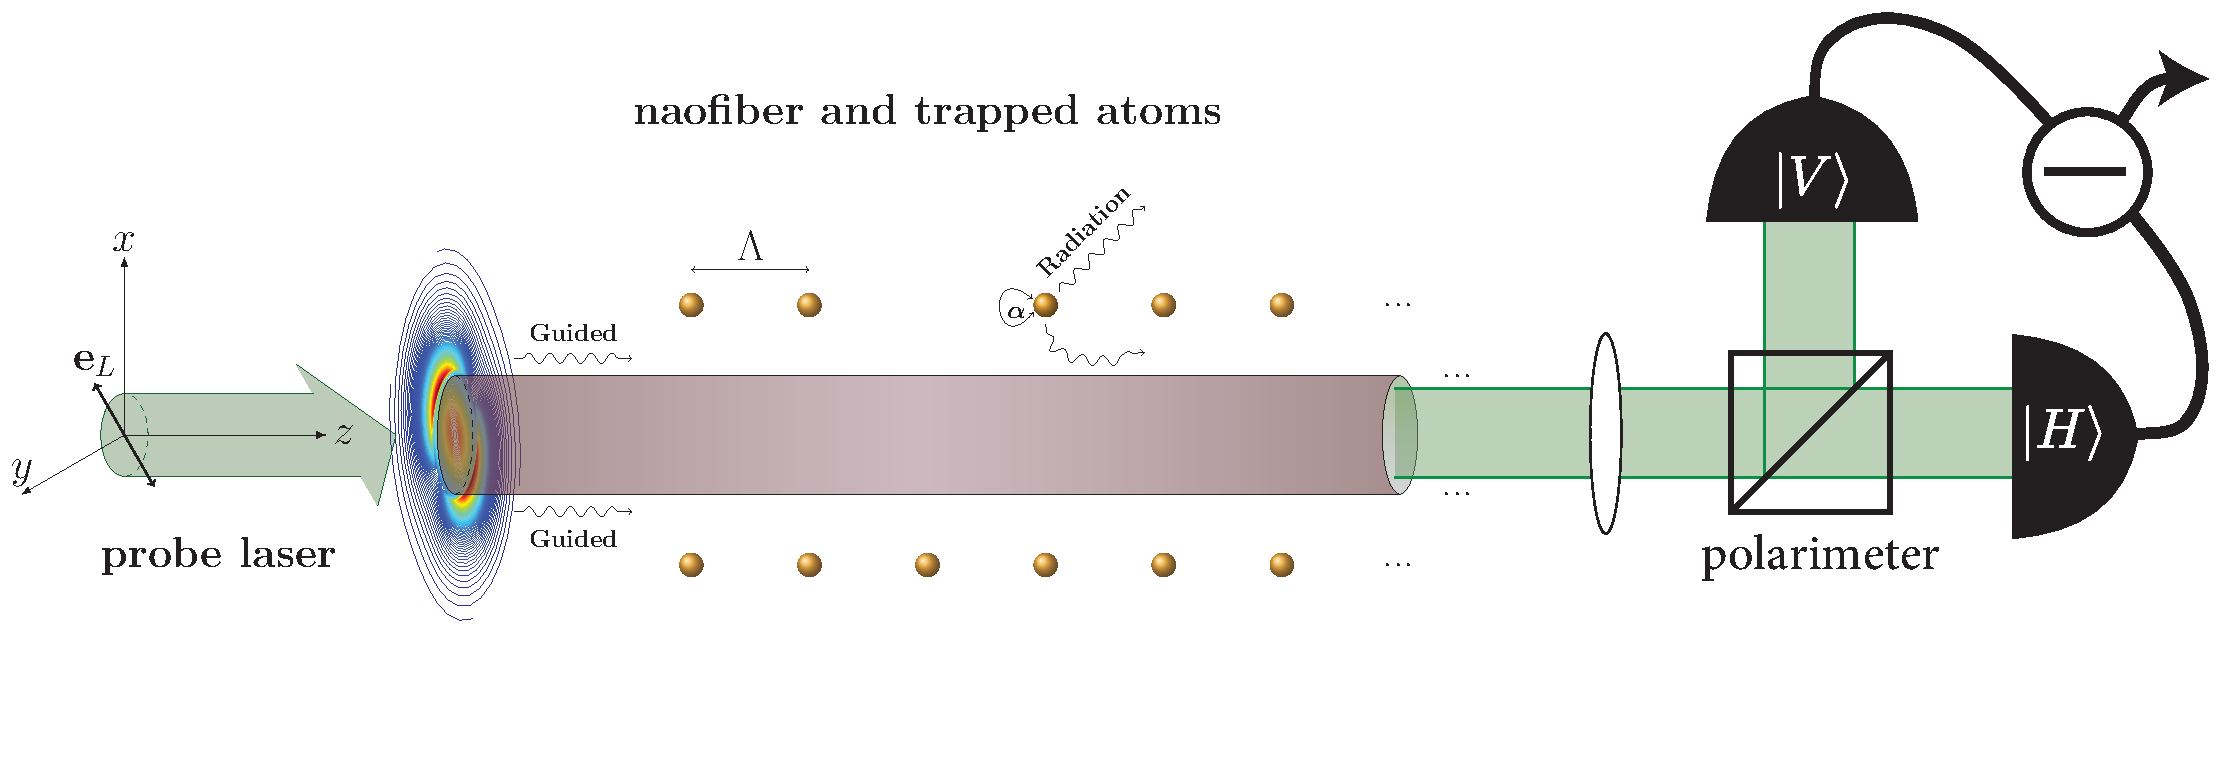
\includegraphics[scale=0.35]{./Figs/BirefringenceMeasurement_randomAtoms}
\subfloat[]{\label{fig:nanofiber_tikz}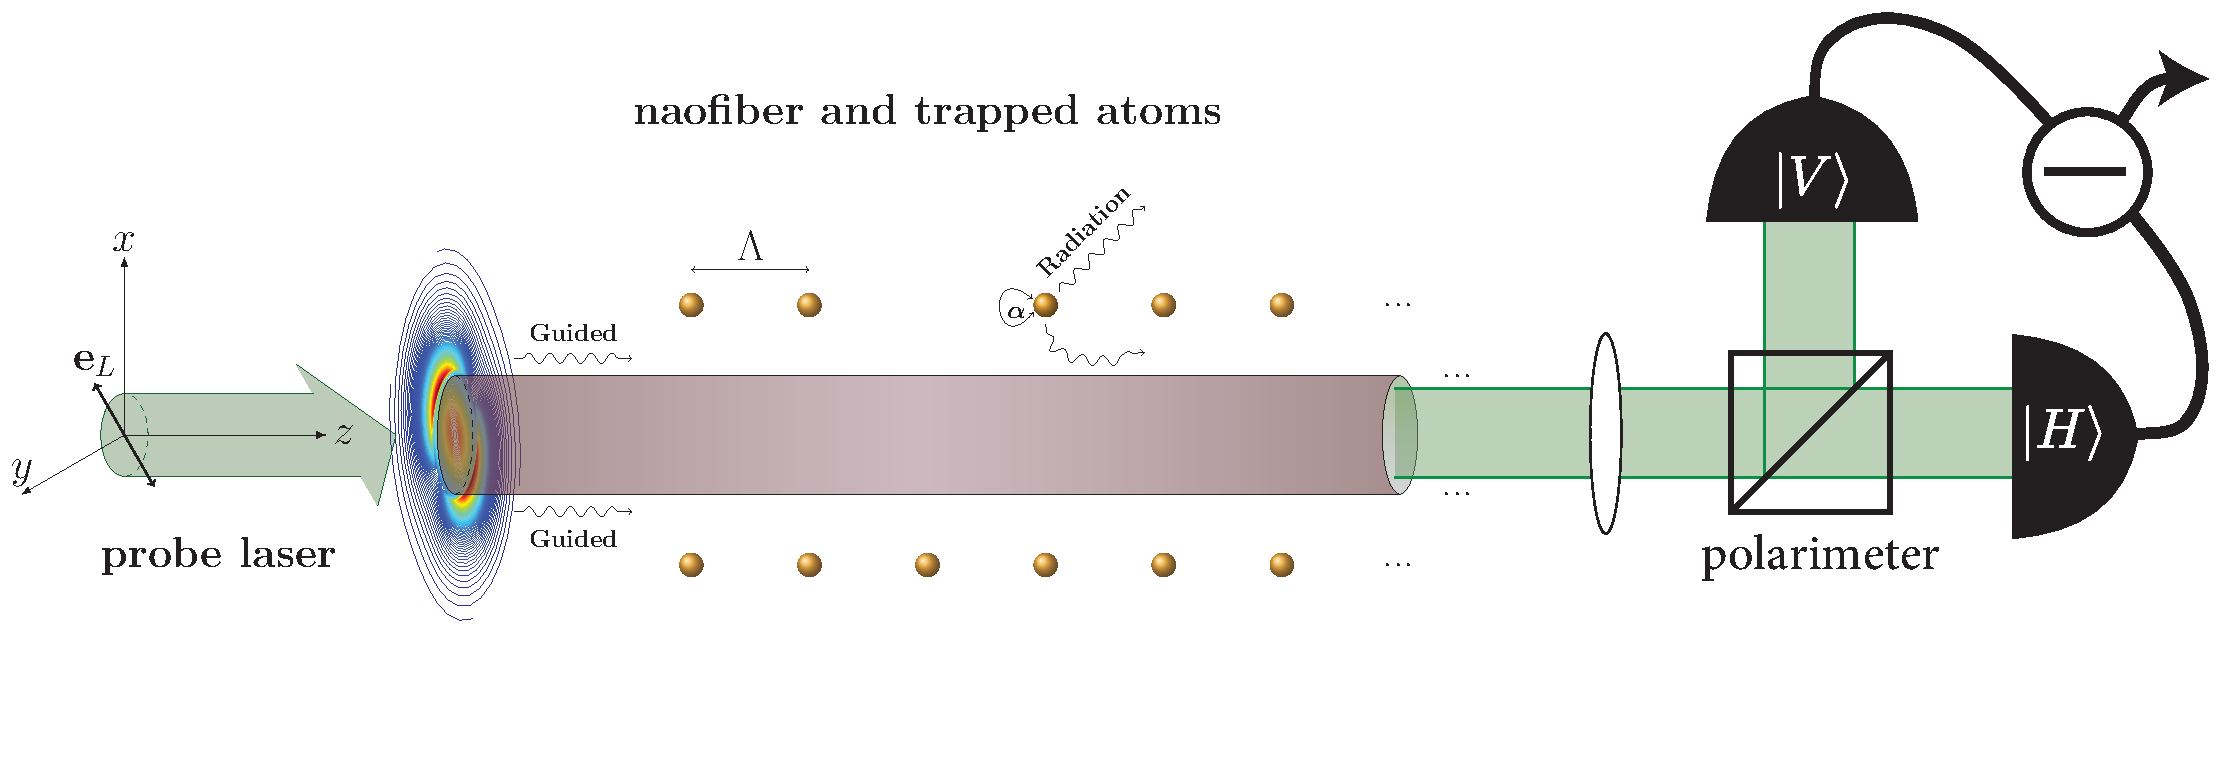
\includegraphics[scale=0.35]{./Figs/BirefringenceMeasurement_randomAtoms}}
\end{minipage}
\par\medskip
\begin{minipage}{0.95\linewidth}
\centering
\subfloat[]{\label{fig:nanofiber_svg}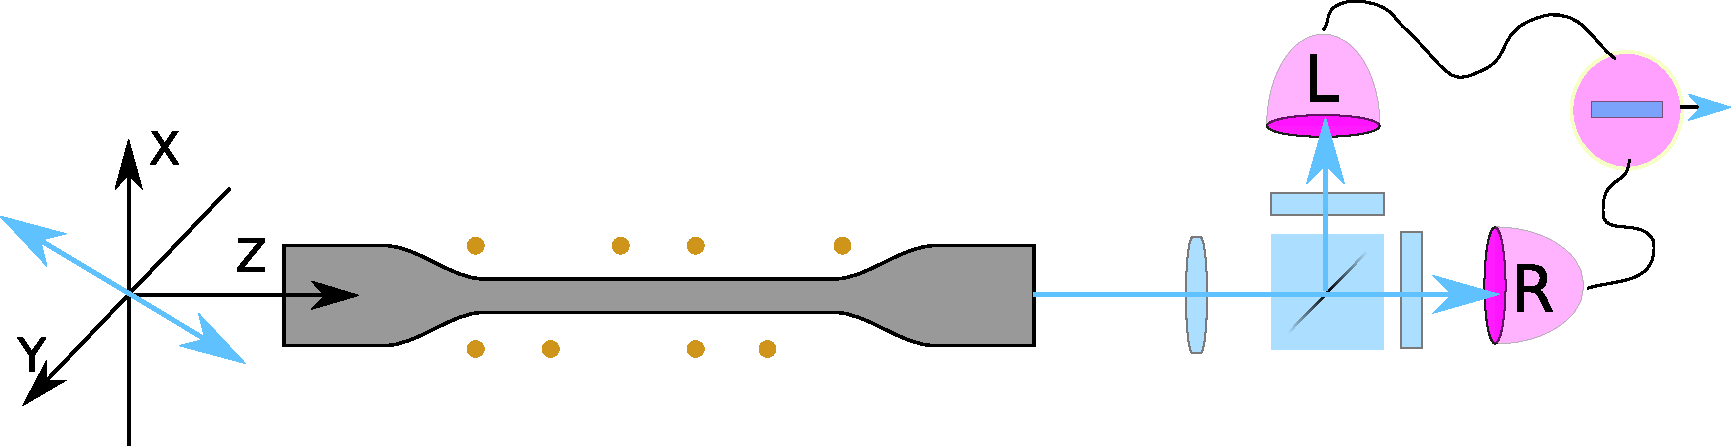
\includegraphics[scale=0.35]{./Figs/ProbeNanofiber_birefringence_lightpath_inputlight}}
\end{minipage}
\caption{Birefringence measurement setup for a nanofiber trapped atomic system. In the evanescent 
field of the nanofiber, atoms (golden balls) randomly  occupy the periodic trapping sites on both sides of 
the \emph{x}-axis in the tapered region shown in the figure.
We assume the nanofiber has a radius constant $ a=225 $nm in this paper.
\comment{Need to choose one of them.}}
\label{fig:BirefringenceMeasurement}
\end{figure}

%========GREEN'S FUNCTION AND INPUT/OUTPUT RESPONSE=========%
\section{Dyadic Green's function and input-output field response}

Given a point particle with tensor polarizability $\tensor{\boldsymbol{\alpha}}$ at position $\br'$ near the surface of a nanofiber, the total field  at frequency $\omega_0$ is given by the solution to the wave equation, 
	\begin{align}\label{Eq::WaveEquationSource}
		\left[ - \nabla \times\nabla \times + n^2(\br)k_0^2 \right] \mathbf{E}(\br) &= -4\pi  k_0^2 \delta^{(3)}(\br-\br')\,  \tensor{\boldsymbol{\alpha}}\cdot \mathbf{E}(\br),
	\end{align}
where $k_0=\omega_0/c$ and $n(\mbf{r})$ is the spatially varying index of refraction that describes the fiber; Gaussian-cgs units are used throughout.  
For an asymptotic input field $\mathbf{E}_{\inp}(\br)$, the scattering solution to \erf{Eq::WaveEquationSource} is given by the Lippmann-Schwinger equation \cite{wubs_multiple-scattering_2004},
	\begin{align}
		\mathbf{E}_{\out}(\br) &=\mathbf{E}_{\inp}(\br)+\tensor{\mathbf{G}}^{(+)}(\br , \br'; \omega_0)\cdot 
\tensor{\boldsymbol{\alpha}}\cdot \mathbf{E}_{\out}(\br')\\
		&\approx \mathbf{E}_{\inp}(\br)+ \tensor{\mathbf{G}}^{(+)}(\br , \br'; \omega_0) \cdot 
\tensor{\boldsymbol{\alpha}}\cdot \mathbf{E}_{\inp}(\br'), \label{Eq::ScatteredField}
	\end{align}
where in \erf{Eq::ScatteredField} we have made the first Born approximation valid for weak scattering. The fundamental object that fully characterizes the scattered radiation as well as the energy level shift and modified decay rate of a scatterer near the dielectric is the dyadic Green's function, $\tensor{\mathbf{G}}(\br, \br';\omega_0)$. Thus  determines the scattered field from a point dipole at $\br'$, $\mathbf{E}_{\rm scat}(\br)= \tensor{\mathbf{G}}^{(+)}(\br , \br'; \omega_0)\cdot \mathbf{d}$, and satisfies the equation of motion,
	\begin{align} \label{Eq::GreensDiffEq}
		\left[ -\nabla\times\nabla\times + n^2(\mbf{r}) k_0^2 \right] \tensor{\mathbf{G}}(\br, \br';\omega_0) &= -4\pi 
k_0^2 \delta^{(3)}(\mathbf{r}-\mathbf{r}') \unittens,
	\end{align}
where $\unittens$ is the unit tensor.  Typically one uses the Green's function to determine the Purcell effect on resonance \cite{}.  We seek here the off-resonance, dispersive response.  

The solution to the Green's function $\tensor{\mathbf{G}}(\br ,\br' ; \omega_0)$, following from Maxwell's equations,  
has been studied previously \cite{sakoda_optical_1996,sondergaard_general_2001,wubs_multiple-scattering_2004}.  As we are interested here in the forward-scattered components that lead to phase shifts and polarization transformations, we directly calculate $\tensor{\mathbf{G}}(\br ,\br' ; \omega_0)$ through a decomposition into normal modes.  A complete set of eigenmodes in the presence of lossless, anisotropic dielectric are defined according to the procedure of Glauber and Lewenstein~\cite{glauber_quantum_1991}.  We seek the eigenmodes $\eigenf(\mathbf{r})$, indexed by $\fidx$, that satisfy the homogeneous wave equation in the absence of sources, i.e. \erf{Eq::WaveEquationSource} for $\tensor{\boldsymbol{\alpha}} = 0$.  To do so, one defines functions $\eigeng(\mbf{r}) \equiv n(\br) \eigenf(\mbf{r})$ that form a complete basis, as they are eigenfunctions of the Hermitian operator, $\mathcal{H}(k_0) = -\frac{1}{n(\br)} \nabla\times\nabla\times \frac{1}{n(\br)} + k_0^2$, according to $\mathcal{H}(k_0)  \eigeng(\mbf{r}) = \lambda_\fidx \eigeng(\mbf{r})$. The eigenvalue, $\lambda_\fidx= k_0^2-k_\fidx^2$, determines the wavenumber for a given mode, $k_\fidx$.  We are interested specifically in the transverse functions, $\nabla \cdot \eigeng(\br) = 0$, with eigenvalues $\lambda_n \neq 0$.  These fall into two categories, guided and unguided (radiation) modes. \comment{(what about the ``whispering gallery" modes?)}.  
%Modes whose transverse wavevector is purely imaginary outside the dielectric are guided, while the radiation (unguided) modes do not have this restriction. 
These form a complete, orthonormal set for transverse vector functions,
	\begin{align}
	\int \mathrm{d}^3\br \, \eigeng^*(\mbf{r}) \cdot \eigengp(\mbf{r})  &= \int \mathrm{d}^3\br \, n^2(\br) \eigenf^* (\br)\cdot  \eigenfp(\br) =\delta_{\fidx, \fidx'},\label{Eq::Orthogonality}\\
	\sum_\fidx \eigeng(\br) \eigeng^*(\br') &= \sum_\fidx n(\br)n(\br') \eigenf(\br) \eigenf^*(\br') =\tensor{\delta}^{(T)}(\br-\br')  \unittens, \label{Eq::Completeness}
	\end{align}
where $\tensor{\delta}^{(T)}(\br-\br')$ is the delta function for transverse vector fields.  
%When the eigenfunctions form a continuous set, the sum over $\fidx$ in \erf{Eq::Completeness} represents an integral and likewise the discrete Kroenecker delta function in \erf{Eq::Orthogonality} represents a Dirac delta function.  
It follows that the transverse dyadic Green's function can be decomposed in terms of the eigenfunctions~\cite{sakoda_optical_1996, sondergaard_general_2001}
	\begin{align}
		\tensor{\mathbf{G}}^{(T)}(\br,\br'; \omega_0)%& = -4\pi k_0^2 \sum_{\fidx} \frac{ n(\br) n(\br') \eigenf (\br) 
%\eigenf^* (\br')}{\lambda_\fidx}, \\
	&= -4\pi \sum_{\fidx} \frac{  \omega_0^2 \eigenf (\br) 
\eigenfp^* (\br')}{\omega_0^2-\omega_\fidx^2},
	\end{align}
where the eigenvalues appear as $\omega_\fidx^2 = c^2 k_\fidx^2$.  The sum includes both guided and unguided contributions. We focus here on the guided-mode contribution to the Green's function. 
%Details concerning the radiation modes of a nanofiber can be found in Refs. \cite{Snyder and Love, sondergaard_general_2001,le_kien_spontaneous_2005}.

We treat an optical nanofiber of radius $a$ as having step-index profile,
	\begin{align} \label{Eq::IndexofRefraction}
		n(r_\perp) = \Bigg\{  
			\begin{array}{l l} n_1 & \quad r \leq a \\
						 n_2 & \quad r > a 
		\end{array},
	\end{align}
for a silica core ($n_1 = 1.45$) and infinite vacuum cladding ($n_2 = 1$).  For a cylindrically symmetric dielectric the guided modes are $\eigenf (\br) = \mathbf{u}_\mu (\br_\perp) e^{i\beta z}/\sqrt{2 \pi}$, with indices $\mu=\{j, \beta, p\}$ for guided mode $j$ with propagation constant $\beta$ and polarization $p$.  The transverse mode functions are normalized according to $\int d^2 \mbf{r}_\perp \, n^2(r_\perp)\mathbf{u}^*_\mu (\br_\perp) \cdot \mathbf{u}_{\mu'} (\br_\perp)\big|_{\beta = \beta'} = \delta_{j,j'}\delta_{p,p'}$ and have units $1/\sqrt{A}$ \cite{le_kien_anisotropy_2014}.  Two convenient guided-mode bases are the quasilinear and quasicircular polarization modes, given in  Appendix \ref{Appendix::ModeFunctions}, whose $z$-components satisfy the two-dimensional Schr\"{o}dinger-like equation, $\big[\nabla_\perp^2 +k_0^2 n^2(r_\perp) \big] u_{\mu,z} (\br_\perp) = \beta^2 u_{\mu,z} (\br_\perp)$ \cite{kien_field_2004}.  

We consider nanofibers that support only the lowest HE$_{11}$ guided modes at the relevant frequency $\omega_0$ ~\cite{Yariv}, and thus we drop the mode index $j$.  In this case there are four guided modes: two polarizations $p$, each with propagation constant (longitudinal wavenumber) $\beta(\omega_0) = \pm\beta_0$ corresponding to forward and backward propagation.  
%The value of $\beta_0$ is found by enforcing the boundary conditions at the fiber surface and solving the eigenvalue equation \cite{Yariv, Marcuse, SnyderLove}. 
The guided-mode contribution to the dyadic Greens function is then 
	\begin{equation} \label{Eq::GreensEigenmodes}
		\tensor{\mathbf{G}}_g(\br,\br'; \omega_0) = \int_{-\infty}^\infty \frac{d \beta}{2 \pi} \sum_{p} 
\frac{-4\pi\omega_0^2}{\omega_0^2-\omega^2(\beta)} \mathbf{u}_{\beta,p} (\br_\perp)\mathbf{u}^*_{\beta,p} 
(\br_{\perp}^\prime) e^{i\beta(z-z')},
	\end{equation}
where $ \omega(\beta)$ is the frequency of the guided HE$_{11}$ for a given $\beta$.  
%The HE$_{11}$ mode has no cutoff; for a given $\omega$, there always exists a guided mode with propagation constant $\beta(\omega)$.  

For $z>z'$ ($z<z'$), the contribution of the guided modes to the retarded (causal) Green's function is found by the 
usual displacement of the pole on the positive (negative) $\beta$-axis into the upper (lower) half of 
the complex plane. The result is \cite{manga_rao_single_2007}
	\begin{align} 
		\tensor{\mathbf{G}}^{(+)}_g(\br,\br'; \omega_0) = &2\pi i \sum_{f,p}  {\rm Res}\vert_{\beta =f\beta_0} 
\left[\frac{-4\pi \omega_0^2 }{2\pi ( \omega_0^2-\omega^2(\beta))}\right]  \mathbf{u}_{f\beta_0, p} 
(\br_\perp)\mathbf{u}^*_{f\beta_0, p} (\br_{\perp}^\prime)e^{if \beta_0 (z-z')} \nonumber \\
= & 2\pi i \frac{\omega_0}{v_g } \sum_{f,p} \mathbf{u}_{f, p} (\br_\perp)\mathbf{u}^*_{f , p} 
(\br_{\perp}^\prime) e^{i f \beta_0(z-z')} \Theta \big( (z-z')f \big), \quad \quad \change{(\mbf{r} \neq \mbf{r}')} \label{Eq::GreensGuided}
	\end{align}
where $f=\pm$ indicates the propagation direction, $v_g= \vert d\omega/d\beta \vert_{\beta=\beta_0}$ is the group velocity at $\omega_0$, and $\Theta \big( (z-z')f \big)$ is a Heaviside function enforcing causality for the forward- and backward-scattered fields. In the second line, we have suppressed the label $\beta_0$ as it is implicit in the definition of the guided modes at frequency $\omega_0$. 

Radiative properties of a scatterer (the decay rate and energy level shift) are determined by evaluation of the dyadic Green's function at the source point $\mbf{r} = \mbf{r}'$ \cite{fussell_decay_2005}.  However, for $z=z'$ we cannot close the contour. Instead, we expand the resonant denominator in \erf{Eq::GreensEigenmodes} with the poles moved to yield the retarded (causal) response,
\begin{equation}
\frac{1}{(\omega_0+i\epsilon)^2-\omega^2(\beta)}=\frac{1}{2 \omega(\beta)}\left[ \frac{1}{\omega_0+ i 
\epsilon - \omega(\beta)} - \frac{1}{\omega_0+ i \epsilon + \omega(\beta)} \right],
\end{equation}
 and employ the usual distribution identities \cite{sondergaard_general_2001},
\begin{equation}
\lim_{\epsilon \rightarrow 0_+} \frac{1}{\omega_0 + i \epsilon \mp 
\omega(\beta)}=\mathcal{P}\left[\frac{1}{\omega \mp \omega(\beta)} \right] + i \pi \delta (\omega_0 \mp 
\omega(\beta)).
\end{equation}
Only the positive-frequency component contributes to the $\delta$-function, and it follows that the imaginary part of the Green's function at $\br = \br'$ that determines the resonant ($\omega_0 = \omega_{eg}$) Purcell enhancement of spontaneous emission into the guided modes is \cite{dung_spontaneous_2000, fussell_decay_2005, chen_finite-element_2010}
	\begin{equation}\label{Eq::ImGreenLocal}
		\Im \big[\tensor{\mathbf{G}}^{(+)}_g(\br',\br'; \omega_{eg}) \big] = \pi \frac{\omega_{eg}}{v_g } \sum_{f, p} 
		\mathbf{u}_{f, p} (\br_{\!\perp}^\prime)\mathbf{u}^*_{f , p} (\br_{\!\perp}^\prime).
	\end{equation}
The energy level shift of the scatterer due to its proximity to the dielectric is found from the real part of the Green's function at $\br = \br'$. 
To find the total modified spontaneous emission rate and energy level shift one must include the unguided radiation modes \cite{le_kien_spontaneous_2005} or employ other representations of the Green's function \cite{klimov_spontaneous_2004}.  

Equation (\ref{Eq::GreensGuided}) is the central result from which we can calculate the dispersive response.  Consider a forward-propagating ($f=+$) input field in the guided modes with frequency $\omega_0$, positive-frequency amplitude $\Eamp$, and arbitrary polarization, $\mathbf{E}^{(+)}_{\inp}(\br) = \Eamp  \mathbf{u}_{\rm in}(\br_\perp) e^{i \beta_0 z}$.   
The effective mode area at the atom's position is determined from the total cycle-averaged power transported along the nanofiber, $P_{{\rm in},z} = (v_g/2\pi) \int d^2\br |\mathbf{E}^{(+)}_{\inp}(\br) |^2$, and the intensity at the atom, $I_{\rm in}(\mathbf{r}') = (c/2\pi) |\mathbf{E}^{(+)}_{\inp}(\br) |^2$,\comment{we'll discuss factors of $2\pi$ or $ 8\pi $} via the relation \cite{domokos_quantum_2002},
 	\begin{align} \label{Eq::AreaIn}
 		A_{\rm in} \equiv \frac{P_{{\rm in}}}{I_{\rm in}(\mathbf{r}')} = \frac{1}{n_g |\mathbf{u}_{\rm in}(\mathbf{r}'_\perp)|^{2}},
	\end{align}
where $n_g = c/v_g$ is the group index of refraction.  Tight confinement of the guided modes in the nanofiber results in significant intensity near the nanofiber for relatively small input power \cite{bures_power_1999}.  
%Note that $P_{\rm in}$ is not the total power, since some of the energy is azimuthally transported around the nanofiber due to the longitudinal component of the guided modes \cite{le_kien_scattering_2006}.\comment{This is true but an aside that is not relevant}.

Substitution of the guided-mode Green's function, \erf{Eq::GreensGuided}, into the Lippman-Schwinger equation, \erf{Eq::ScatteredField}, yields the transmitted (forward-scattered) and reflected (backward-scattered) output fields, $\mathbf{E}_{\out}(\br) = \Eamp \big[ \mathbf{u}_{\trans, \out} (\br_\perp) e^{i \beta_0 z} + \mathbf{u}_{\refl,\out} (\br_\perp) e^{-i \beta_0 z} \big]$, 
	\begin{align}
		\mathbf{u}_{\trans, \out} (\br_\perp) &=  \sum_{p,p'}  \, c_{p} t_{pp'} \mathbf{u}_{\fwd, p'}(\br_\perp) \\ 
		\mathbf{u}_{\refl,\out} (\br_\perp) &=  \sum_{p,p'}  \, c_{p} r_{pp'} \mathbf{u}_{\bwd, p'}(\br_\perp),
	\end{align}
where we have decomposed the input into the polarization eigenmodes, $\mbf{u}_{\rm in}(\mbf{r}_\perp) = \sum_{p} c_{p} \mathbf{u}_{\fwd,p}(\br_\perp)$.  
For an atom located at $\br'$, and $z>z'$, the transmission and reflection matrices are 
	\begin{align} \label{Eq::PolarizationTransformation}
		t_{pp'} =& \delta_{p,p'} +  2\pi i k_0 n_g \, \mathbf{u}^*_{+, p'}(\br'_\perp) \cdot 
\tensor{\boldsymbol{\alpha}} \cdot \mathbf{u}_{+, p}(\br'_\perp) , \\
		r_{pp'} =&  2\pi i k_0 n_g \, \mathbf{u}^*_{\bwd, p'}(\br'_\perp) \cdot 
\tensor{\boldsymbol{\alpha}} \cdot \mathbf{u}_{\fwd, p}(\br'_\perp) e^{2 i\beta_0 z'} , 
	\end{align} 
We focus here on the transmitted fields whose interference with the input field for $z>z'$ results in a phase shift and a polarization transformation.  
For weak scattering the diagonal terms, $t_{p p} \approx \sqrt{1-R_p}e^{i \delta \phi_p}$, determine the phase shift and attenuation due to reflection induced on each mode,
	\begin{align}
		 \delta \phi_p &= \frac{2 \pi k_0}{A_{\rm in}} \Re(\alpha_{pp}),  \label{Eq::PhaseShift} \\
		R_p &=  \frac{4 \pi k_0}{A_{\rm in}} \Im(\alpha_{pp}) .\label{Eq::Attenuation} 
	\end{align} 
Here, the $\{p,p'\}$-element of the tensor polarizability is given by, $\alpha_{pp'} \equiv \mathbf{e}^*_{p'} \cdot \tensor{\boldsymbol{\alpha}}\cdot \mathbf{e}_{p}$, with units vectors for each of the forward-propagating mode functions, $\mathbf{e}_{p}\equiv \mathbf{u}_{+,p}(\br'_\perp)/|\mathbf{u}_{+,p}(\br'_\perp)|$. 

The phase shift per atom, \erf{Eq::PhaseShift}, is modified over free space in two ways, both of which are captured by the effective mode area $A_{\rm in}$. 
First, although material dispersion in an optical fiber is negligible, an atom coupling to a tightly confined guided mode can lead to additional waveguide dispersion and a significant reduction in the group velocity.  
Such ``slow light" enhances the atom-photon coupling strength. In the nanofiber geometry, this effect is moderate -- the group index $n_g \approx 1.4$ for atoms trapped at $r' \approx1.5 a$. 
Second and more importantly,  the tight spatial confinement of the guided mode means strong cooperativity, as measured by the ratio the scattering cross section to the mode area, for all atoms trapped along the nanofiber.  

In contrast, diffraction restricts the collective phase shift for an ensemble of atoms in free space~\cite{baragiola_three-dimensional_2014}.  
For a Gaussian beam with beam waist $w_0$, the total phase shift induced by a collection of polarizable atoms will be $\delta \phi = N_{\eff} 2 \pi k_0\Re({\alpha})/A$, where $A = \pi w^2_0$ is the beam area at the focus and $N_{\eff}$ is the effective number of atoms that radiate into this mode.  
One can couple more strongly to few atoms at the center of a tightly focusing the beam or couple weakly to many atoms by choosing a larger focus which has a larger focal volume, but hence, smaller cooperativity per atom.  
This trade-off is illustrated Fig. ?.  
In  \frf{Fig::PhaseShift}(b),  we compare the total phase shift and phase shift per atom (see Fig. 5.4 of my thesis) for the nanofiber and for a 3D Gaussian cloud in free space for varying probe waists. 

The off-diagonal terms in the transmission matrix, Eq. (?), describe the polarization transformation. For example, if we take the polarization of the modes to be the quasilinear, given in \erf{Eq::QuasilinearModes} ($p = H,V$), then $t_{HV} \equiv \chi_{\rm Far}$ is the rotation angle of the Faraday effect \cite{}.  The phase difference in that basis, $\delta  \phi_H - \delta \phi_V$, corresponds to birefringence induced on the guided mode.  
%Alternatively, analyzed in the quasicircular modes given in \erf{Eq::QuasicircularModes} ($p=\pm$), the differential phase $\delta \phi_+ -\delta  \phi_-$ corresponds to Faraday rotation and $t_{+-}$ to birefringence.  
We make use of such polarization transformations as a means to nondestructively measure the atoms and generate collective spin squeezing.
\comment{How does our scattering matrix relate to that from Le Kien's results about propagation of light through an array of nanofiber-trapped atoms?  Specifically, Eq. (8) of Ref. \cite{le_kien_correlations_2008} and/or Eqs. (8-10) of Ref. \cite{le_kien_propagation_2014}?  
}

%========= FIGURE: Geometry (coupling strength, magic wavelength, area and detuning) =========%
\begin{figure}
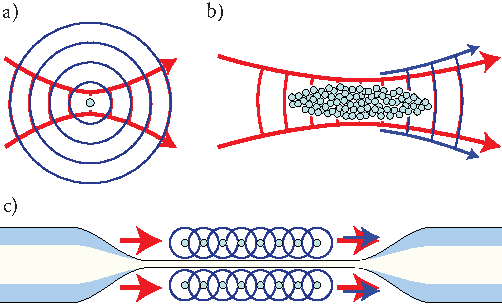
\includegraphics[scale=1.00]{./Figs/Fig_ModeMatch}
%\begin{minipage}{.32\linewidth}
%\centering
%\subfloat[]{\label{fig:D1_magicfreqs44_transition}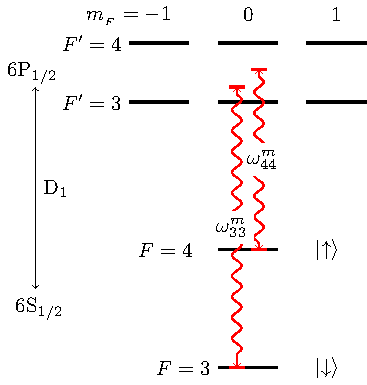
\includegraphics[scale=0.65]{./Figs/D1_magicfreqs44_transition}}
%\end{minipage}
%\begin{minipage}{.32\linewidth}
%\centering
%\subfloat[]{\label{fig:domega_magic12_q_NA2500_r1d8a}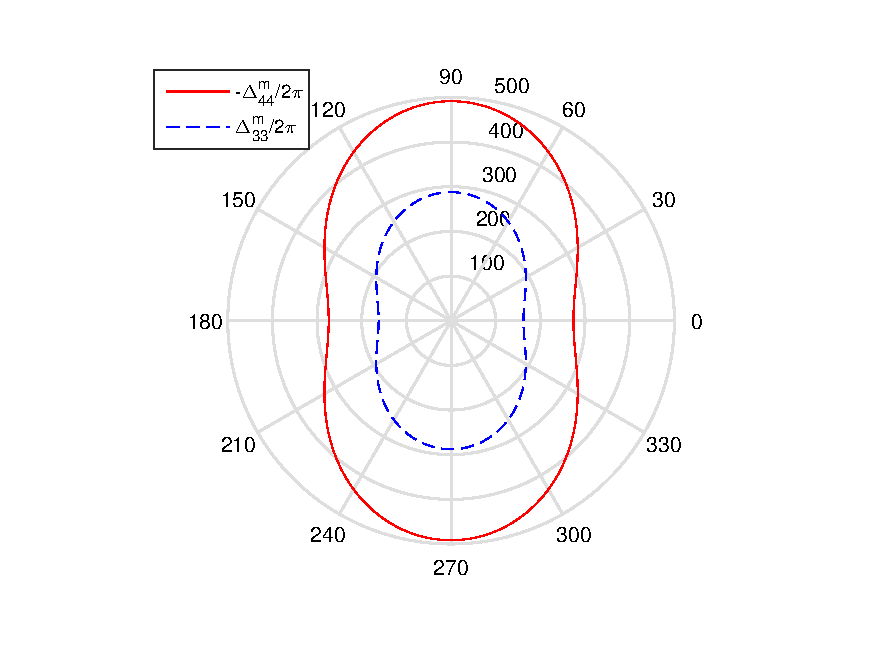
\includegraphics[scale=0.4]{./Figs/domega_magic12_q_NA2500_r1d8a}}
%\end{minipage}
%\begin{minipage}{.32\linewidth}
%\centering
%\subfloat[]{\label{fig:kappa_q_D1_xyplane_NA2500_r1d8a_m44}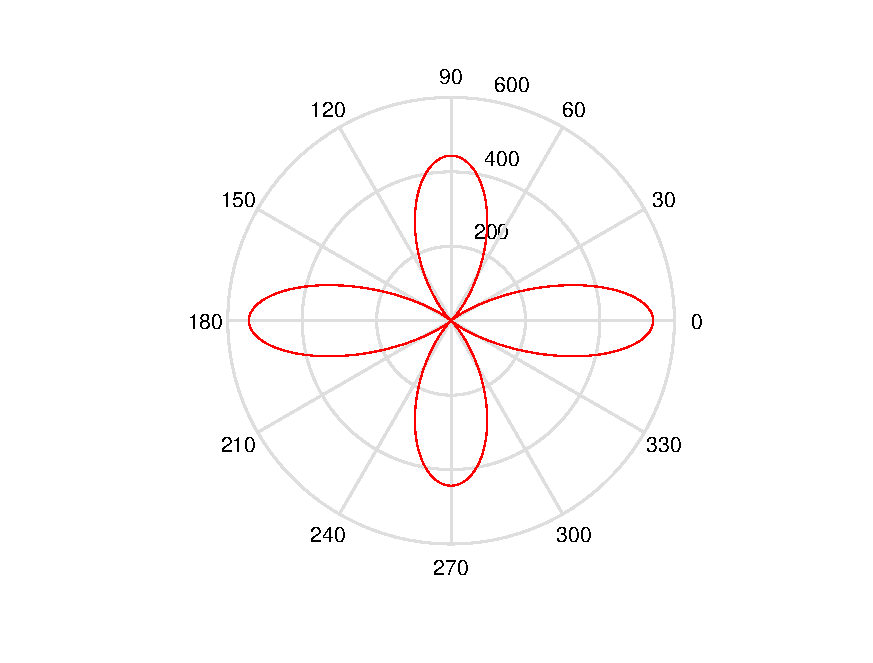
\includegraphics[scale=0.4]{./Figs/kappa_q_D1_xyplane_NA2500_r1d8a_m44}}
%\end{minipage}
\caption{Depiction of mode-matching for various atom-light geometries. (a) Single atom in a tightly focused beam. (b) Rarefied atomic cloud and a paraxial probe beam. (c) 1D optical lattices near the surface of an optical nanofiber interacting with a fiber-guided probe. }\label{Fig::CouplingStrength}
\end{figure}
%=============================================

%============== FIGURE: Phase Shifts =====================%
\begin{figure}
\begin{minipage}{.49\linewidth}
\centering
\subfloat[]{\label{fig:RelEnhanceFactor_r_w10micro}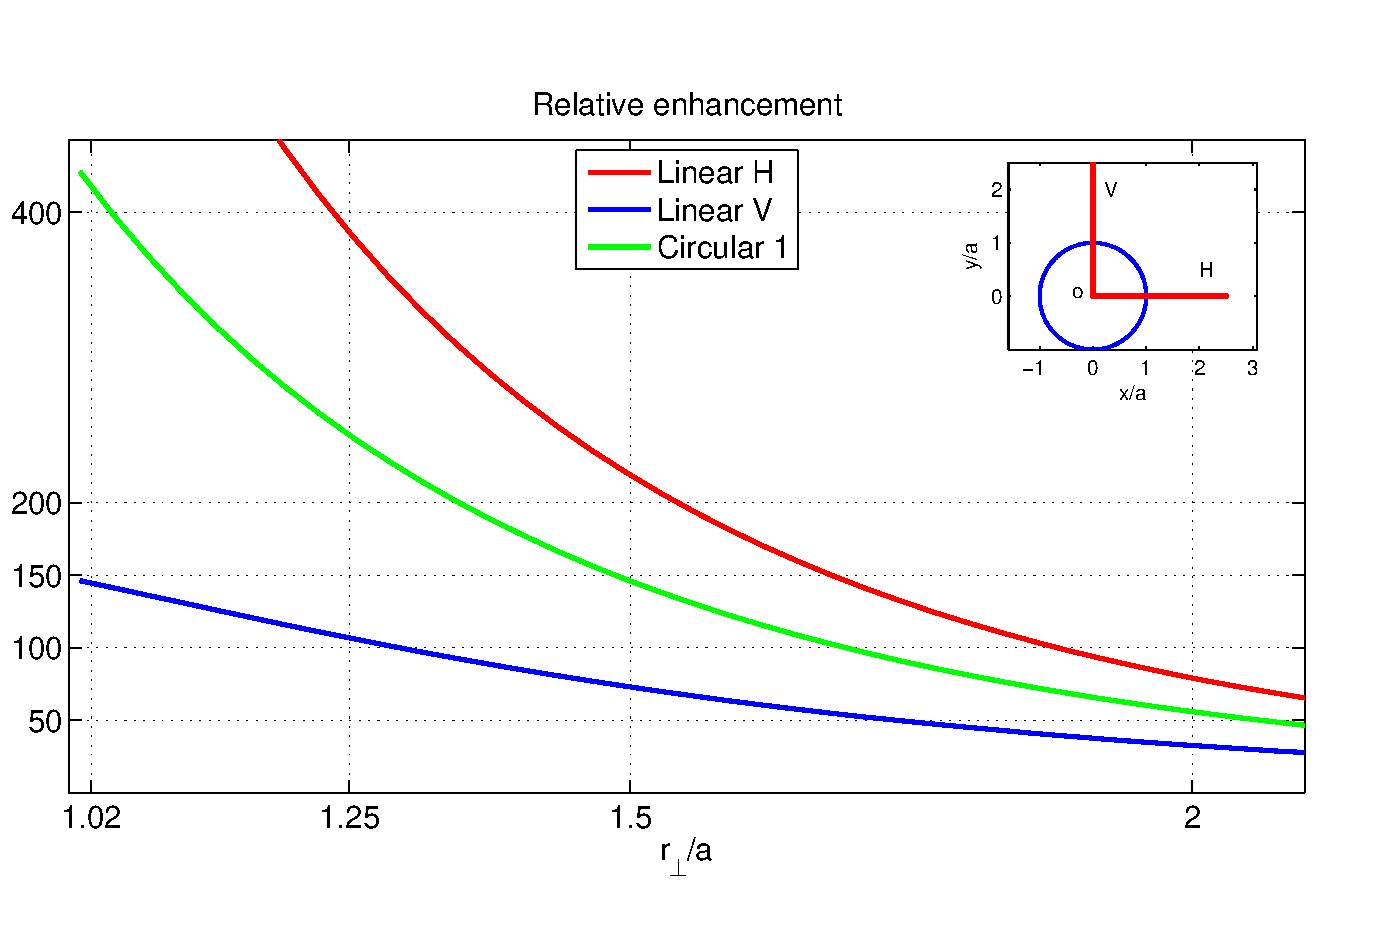
\includegraphics[scale=0.45]{./Figs/RelEnhanceFactor_r_w10micro}}
\end{minipage}
\caption{Dispersive phase shift imparted by scalar scatterers (atoms) near a nanofiber on the \emph{x}-axis compared to phase shift in free space on a paraxial $\mathrm{TEM}_{00}$ beam with waist $w_0 = 30 \mu$m. (a) Peak single-atom phase shift. (b) Average phase shift per atom compared to a three-dimensional Gaussian cloud in free space. }\label{Fig::PhaseShift}
\end{figure}
%=====================================================%

	
	%===================Heisenberg-Langevin Equations=====================%
	\subsection{Heisenberg-Langevin-picture solution and atomic response}
	
The Lippmann-Schwinger solution, \erf{Eq::ScatteredField}, determines the input-output relation for linear atomic response given by the polarizability tensor $\tensor{\alpha}$.  In this section we connect this with the fully quantum mechanical description of dispersive atomic response and input-output relations for the quantized guided modes.  Following \cite{le_kien_spontaneous_2005}, we use a Heisenberg-Langevin approach for one-dimensional systems.  

The positive frequency component of the quantized electric field operator decomposes into guided and radiation (unguided) modes, $\hat{\mathbf{E}}^{(+)}=\hat{\mathbf{E}}_g^{(+)}+\hat{\mathbf{E}}_{r}^{(+)}$, where
	\begin{align}
		\hat{\mathbf{E}}_g^{(+)}(\br) &= \sum_{f,p} \int \mathrm{d}\omega  \sqrt{\frac{ \hbar \omega}{ v_g}} \awg \mathbf{u}_\mu (\br\!_\perp) e^{i f\beta(\omega) z } ,\label{Eq::QuantizedElectricField} \\
		\hat{\mathbf{E}}_r^{(+)}(\br) &= \sum_{m,p} \int \mathrm{d}\omega   \int_{-kn_2}^{kn_2}\mathrm{d}\beta \, \sqrt{ \hbar \omega}\awr \mathbf{u}_\nu (\br\!_\perp) e^{i\beta(\omega) z },
	\end{align}
The four HE$_{11}$ guided modes at each frequency $\omega$ are indexed by $\mu =(\omega, f, p)$ for two polarizations $p$ and two propagation directions $f=\pm1$ with wavenumbers $f\beta (\omega)$.  
The radiation modes are indexed by  $\nu=(\omega, \beta, m, p)$ where $m$ is the azimuthal quantum number (angular momentum), $p$ labels the two orthogonal polarizations. The longitudinal propagation constant $\beta(\omega)$ can vary from $-kn_2$ to $kn_2$, with $k = \omega/c$ \cite{sondergaard_general_2001,le_kien_spontaneous_2005}.  
The creation/annihilation operators satisfy the usual continuous-mode commutation relations, $[\hat{a}_\mu, \hat{a}^\dag_{\mu'} ] = \delta_{f,f'} \delta_{p,p'} \delta ( \omega - \omega ') $, $[\hat{a}_\nu ,\hat{a}^\dag_{\nu'} ] = \delta_{m,m'} \delta_{p,p'} \delta ( \omega - \omega ')  \delta ( \beta - \beta') $.

The Hamiltonian for the system is
\begin{equation}
\hat{H} = \hat{H}_F+\hat{H}_A + \hat{H}_{\inter}.
\end{equation}
The free field Hamiltonian decomposes into guided and unguided modes, 
	\begin{equation}
		\hat{H}_F = \sum_{f,p}\int \mathrm{d}\omega \, \hbar \omega \hat{a}^\dagger_\mu \hat{a}_\mu 
+\sum_{m,p} \int \mathrm{d}\omega  \int_{-k n_2}^{k n_2} \mathrm{d}\beta \, \hbar \omega 
\hat{a}^\dagger_\nu \hat{a}_\nu.
	\end{equation}
We consider here alkali atoms with hyperfine multiplets of ground and excited levels, $\{ 
\ket{g}=\ket{nS_{1/2}, F, M_F}\}$, $\{ \ket{e} =\ket{nP_{J'}, F', M_{F'}}\}$,
	\begin{equation}
		\hat{H}_A  = \sum_g E_g \hat{\sigma}_{gg} + \sum_e E_e \hat{\sigma}_{ee},
	\end{equation}
with atomic transition operators $\hat{\sigma}_{ij} \equiv \ket{i}\bra{j}$.  In the rotating wave approximation, the atom-field interaction Hamiltonian is
	\begin{align}
		\hat{H}_{\inter} &= -\hat{\mathbf{d}}\cdot \hat{\mathbf{E}} =- \sum_{e,g} \left[ \hat{\mathbf{d}}_{eg}\cdot 
\hat{\mathbf{E}}^{(+)}(\br')+\hat{\mathbf{d}}_{ge}\cdot \hat{\mathbf{E}}^{(-)}(\br') \right],
	\end{align}
where the atomic dipole operator is projected between excited and ground subspaces, $\hat{\mathbf{d}}_{eg}= \hat{P}_e \hat{\mathbf{d}} \hat{P}_g $. The interaction Hamiltonian then takes the form, 
\begin{equation}
	\hat{H}_{\inter} = -\sum_{e,g} \left(\sum_{f,p} \int\mathrm{d}\omega \; \hbar g_{\mu, e,g}\, \hat{a}_\mu  \, 
		\hat{\sigma}_{eg}+ \sum_{m,p} \int\mathrm{d}\omega \! \int_{-kn_2}^{kn_2}\mathrm{d}\beta \,  \hbar 
g_{\nu, e,g}\, \hat{a}_\nu \, \hat{\sigma}_{eg}\right) + {H.c.},
	\end{equation}
where the coupling constants for guided/radiation modes are
\begin{subequations} \label{Eq::CouplingConstants}
	\begin{align}
		\hbar g_{\mu, e,g} &= \sqrt{\frac{\hbar \omega}{ v_g  }}\, \bra{e} \hat{\mathbf{d}} \ket{g} 
\cdot\mathbf{u}_\mu ( \error{\br'\!_\perp} ) e^{i f \beta(\omega)z} , \\
		\hbar g_{\nu, e,g} &= \sqrt{  \hbar \omega } \, \bra{e} \hat{\mathbf{d}} \ket{g} \cdot \mathbf{u}_\nu ( \error{ \br'\!_\perp} ) e^{i\beta(\omega)z}  .
	\end{align}
\end{subequations}
The Heisenberg equations of motion thus follow:
	\begin{align}
		\der{\hat{a}_\mu} &= -i\omega \hat{a}_\mu +i\sum_{e,g} g_{\mu, e,g}^* \hat{\sigma}_{ge} \label{eq:da}\\
		\der{\hat{a}_\nu} &= -i\omega \hat{a}_\nu +i\sum_{e,g} g_{\nu, e,g}^*  \hat{\sigma}_{ge}\label{eq:danu}\\
		\der{\hat{\sigma}_{ge}} &= -i\omega_{eg} \hat{\sigma}_{ge} \label{Eq::dsigma}  \\
			&+ i\!\int_0^{\infty}\!\!\!\!\! \mathrm{d}\omega \sum_{e',g'} \bigg[ \big(\delta_{ee'} \hat{\sigma}_{gg'} \!-\! \delta_{gg'} \hat{\sigma}_{e'e} \big) \bigg\{ \sum_{f,p}  g_{\mu, e',g'}\hat{a}_\mu (\omega; t) \!+\! \sum_{m,p} \!\int_{-kn_2}^{kn_2}\!\!\!\!\!\! \mathrm{d}\beta \; g_{\nu, e',g'} \hat{a}_\nu(\omega, \beta; t) \bigg\} \bigg]. \nonumber
	\end{align}
Integrating the field equations, 
\begin{subequations}\label{eq:aout1}
\begin{align}
\hat{a}_\mu(\omega; t) &= \hat{a}_\mu(\omega; t_0) e^{-i\omega (t-t_0)} +i \sum_{e,g} g_{\mu,e,g}^* \int_{t_0}^t 
\mathrm{d} t' e^{-i\omega (t-t')}\hat{\sigma}_{ge}(t') \label{Eq::aguidedEOM}
\end{align}
\begin{align}
\hat{a}_\nu (\omega; t) &= \hat{a}_\nu (\omega; t_0) e^{-i\omega (t-t_0)} +i \sum_{e,g} g_{\nu,e,g}^* \int_{t_0}^t \mathrm{d} 
t' e^{-i\omega (t-t')}\hat{\sigma}_{ge}(t'),
\end{align}
\end{subequations}
substituting into \erf{Eq::dsigma}, and making the usual Markov approximation~\cite{?} gives an expression for the ground-excited state coherences,
\begin{align}
&\dt{\hat{\sigma}_{ge}} =-i\omega_{eg} 
\hat{\sigma}_{ge}-\sum_{e'}\frac{\Gamma_{ee'}}{2}\hat{\sigma}_{ge'}  \\
&+i \sum_{e',g'}\bigg[ (\delta_{e,e'} \hat{\sigma}_{gg'} - \delta_{g,g'} 
\hat{\sigma}_{e'e})\int_0^{\infty}\!\!\!\!\!\mathrm{d}\omega \bigg\{\sum_{f,p}  g_{\mu, e',g'} \hat{a}_\mu (t_0) 
+\sum_{m,p}  \int_{-kn_2}^{kn_2}\!\!\!\!\!\mathrm{d}\beta  g_{\nu, e',g'} \hat{a}_\nu(t_0) \bigg\} e^{-i\omega 
(t-t_0)}\bigg], \nonumber
\end{align}
where the decay rates of excited-populations and coherences are given by 
	\begin{equation}
		\Gamma_{ee'} = 2\pi \sum_{\mu,g} g_{\mu,e,g}g^*_{\mu,e',g} \vert_{\omega=\omega_{eg}}+2\pi 
\sum_{m,p,g} \int d\beta \, g_{\nu,e,g}g^*_{\nu,e',g} \vert_{\omega=\omega_{eg}}, \label{Eq::TotaleeDecayRate}
	\end{equation}
and the small energy shift is absorbed into the transition frequency $\omega_{eg} = (E_e - E_g)/\hbar$.  
Equation (\ref{Eq::TotaleeDecayRate}) captures the modification of the spontaneous emission rate due to the nanofiber \cite{le_kien_spontaneous_2005}.  
The first sum describes decay into the guided modes and the second into the unguided radiation modes \cite{ nha_cavity_1997,klimov_spontaneous_2004,le_kien_spontaneous_2005,maslov_distribution_2006}. The decay rate of a given excited state into all guided modes is given by
	\begin{equation}
		\Gamma_e^{\oneD}= 2\pi \sum_{f,p,g} |g_{\mu,e,g} |^2_{\omega = \omega_{eg}} =  \frac{ 2\pi }{\hbar} \frac{ \comment{\omega_{eg}} }{v_g} \sum_{f,p,g} \big|\bra{e}\hat{\mathbf{d}}\ket{g} \cdot \mathbf{u}_{fp}(\br'_\perp)\big|^2  .
	\end{equation}
This is in agreement with the expected expression from the guided-mode contribution to the dyadic Green's function in \erf{Eq::ImGreenLocal},
	\begin{equation} \label{Eq::Gamma1DGreens}
		\Gamma_e^{\oneD} =  \frac{2}{\hbar} \sum_{g}  \bra{g}\hat{\mathbf{d}}\ket{e}\cdot 
\Im \Big[\tensor{\mathbf{G}}^{(+)}_g(\br', \br'; \omega_{eg} ) \Big] \cdot \bra{e}\hat{\mathbf{d}}\ket{g},
	\end{equation}
which is enhanced over the free-space rate by the Purcell factor. The decay rate into a given mode, guided or radiation, depends on the atom's position and dipole orientation \cite{klimov_spontaneous_2004, vos_orientation-dependent_2009}. Recently it was demonstrated that decay rates into the forward and backward guided modes are not always equal \cite{mitsch_quantum_2014}. When the atomic dipole has a component rotating in the plane defined by the atom and nanofiber, the relative decay rates differ due to the broken symmetry arising from the out-of-phase longitudinal component of the guided modes \cite{le_kien_anisotropy_2014}. 

Here we are interested in linear response for excitation far from resonance. We follow Ref. \cite{le_kien_propagation_2014} and consider an atom sufficiently far from the fiber surface such that the modification of the spontaneous emission rate is small.   In this case the decay rate is approximated as $\Gamma_{ee'} \approx \delta_{e,e'} \Gamma_{e}$, where $\Gamma_e$ is the total decay rate from excited state $\ket{e}$, given by the diagonal elements of \erf{Eq::TotaleeDecayRate}.  In steady state, the dipole operator in the linear regime ($\hat{\sigma}_{ee'} \rightarrow 0 $) is approximately
	\begin{align}
		\hat{\sigma}_{ge} \approx -\sum_{g'} \hat{\sigma}_{gg'}\int_0^{\infty}\mathrm{d}\omega \bigg( & \sum_{f,p}  
\frac{g_{\mu, e,g'}}{\omega-\omega_{eg} + i \Gamma_{e}/2  }\, \hat{a}_\mu (t_0) \\
	&+\sum_{m,p} \int_{-kn_2}^{kn_2}\mathrm{d}\beta \, \frac{g_{\nu, e,g'}}{\omega-\omega_{eg} + i \Gamma_{e}/2 } \,\hat{a}_\nu (t_0)  \bigg)e^{-i\omega (t-t_0)} . \nn
	\end{align}
%\comment{In fact, this is obtained by defining $ \hat{\sigma}_{ge'}(t)=\int \frac{\mathrm{d}\omega}{\sqrt{2\pi}}\hat{\sigma}_{ge'}(\omega) e^{-i\omega(t-t_0)} $. } 
By substituting this into \erf{Eq::aguidedEOM} and defining asymptotic modes, \comment{ $\hat{a}^{\inp}(\omega) = \lim_{t_0\rightarrow -\infty} \hat{a}(t_0) e^{i\omega t_0}$, $\hat{a}^{\out}(\omega) = \lim_{t\rightarrow +\infty} \hat{a}(t) e^{i\omega t}$ \cite{fan_input-output_2010}}, we obtain the input-output relationship for the guided modes,
	\begin{align} \label{Eq::aout}
		\hat{a}^{\out}_\mu (\omega) = \hat{a}^{\inp}_\mu (\omega) &- 2\pi i\sum_{p',f'} 
\sum_{e,g,g'}\!\hat{\sigma}_{gg'}\frac{ g_{\mu,e,g}^* g_{\mu',e,g'}}{ \Delta_{eg} + i \Gamma_{e}/2 }\hat{a}^{\inp}_{\mu'}(\omega) \\
&- 2\pi i\sum_{m,p} \sum_{e,g,g'} \int^{kn_2}_{-kn_2} d\beta \,\hat{\sigma}_{gg'}\frac{ g_{\mu,e,g}^* g_{\nu',e,g'}}{ \Delta_{eg} + i \Gamma_{e}/2 }\hat{a}^{\inp}_{\nu}(\omega),\nn
	\end{align}
where $\Delta_{eg} = \omega - \omega_{eg}$. 

This input-output relation contains the phase shift on forward scattered modes as well was attenuation due to elastic scattering into all other modes.
% The real part of this relationship describes the coherent elastic scattering of photons into the forward scattered guided mode $\mu$, mediated by the atomic state.  The imaginary part describes loss from elastic scattering into all other modes.
Equation (\ref{Eq::aout}) agrees with the expected form given by the Lippmann-Schwinger equation in the first Born approximation \footnote{In a careful derivation of the Lippman-Schwinger scattering equation, it is not the total Green's function that appears in \erf{Eq::ScatteredField} but rather a related dyadic quantity, $\mbf{K}(\br,\br', \omega_0) = \mbf{G}(\br,\br', \omega_0) + \delta(\br-\br')/n^2(\br)$ \cite{wubs_multiple-scattering_2004}. 
This function arises by proper accounting of the scatterer's coupling to the \emph{displacement} rather than the electric field \cite{yao_ultrahigh_2009}.  The distinction becomes important at the source point $\mbf{r} = \mbf{r}'$; however, for lossless dielectrics $n(\mathbf{r})$ is real and $\Im[\tensor{\mathbf{G}}(\br',\br'; \omega)] = \Im[\tensor{\mathbf{K}}(\br',\br'; \omega)]$ \cite{yao_-chip_2010}. },
	\begin{equation} \label{Eq::IOScatteredField}
		\hat{\mathbf{E}}^{(+)}_{\out,g}(\br)=\hat{\mathbf{E}}^{(+)}_{ \inp, g}(\br)+\tensor{\mathbf{G}}_g^{(+)}(\br,\br',\comment{\omega_0})\cdot \poltens \cdot \big[\hat{\mathbf{E}}^{(+)}_{\inp, g}(\br')+\hat{\mathbf{E}}^{(+)}_{\inp,r}(\br') \big],
	\end{equation}
by noting
	\begin{align}
		\int d^2 \mbf{r}_\perp \, \mathbf{u}^*_{\mu} (\br_\perp)\cdot \tensor{\mathbf{G}}_g^{(+)}(\br,\br',\comment{\omega_0})\cdot \poltens \cdot \mathbf{u}_{\mu'} (\br'_\perp) &= i \frac{ 2\pi \omega_0}{v_g} \mathbf{u}^*_\mu (\br') \cdot \poltens \cdot \mathbf{u}_{\mu'} (\br') \\
		& = - i \frac{2 \pi}{\hbar} \sum_{e,g,g'}  \hat{\sigma}_{gg'} \frac{g_{\mu,e,g}^* g_{\mu',e,g'}}{ \Delta_{eg} + i \Gamma_{e}/2 }, 
	\end{align}
where the guided-mode dyadic Green's function is given in \erf{Eq::GreensGuided} and the atomic polarizability operator is \cite{buhmann_casimir-polder_2004, deutsch_quantum_2010,kien_dynamical_2013},
	\begin{equation} \label{Eq::PolarizabilityOperator}
		\poltens = - \frac{1}{\hbar} \sum_{e,g,g'}\ket{g}\frac{\bra{g}\hat{\mathbf{d}}\ket{e}\bra{e} 
\hat{\mathbf{d}}\ket{g'}}{\Delta_{eg} + i \Gamma_{e}/2 }\bra{g'}.
	\end{equation}	
%Scattering of classical waves follows when the field is in a coherent state. Injection of a classical field does not alter the Purcell effect or decay rate (which is tied to the atomic transition frequency) it does scatter into all field modes with the same frequency, thus promoting them from vacuum.  
For an atom in ground state $\ket{g}$ and polarization $p$, the phase shift can be expressed as \cite{le_kien_propagation_2014}
	\begin{align} \label{Eq::PhaseShiftMultilevel}
		\delta  \phi_{p,g} =2\pi \frac{\comment{ \omega_{0}}}{v_g} \mathbf{u}^*_{+, p}(\br'_\perp) \cdot \Re\big[\bra{g} 
\hat{\tensor{\boldsymbol{\alpha}}} \ket{g} \big] \cdot \mathbf{u}_{+, p}(\br'_\perp) =& -\frac{1}{\hbar} \sum_e \frac{ \comment{ \omega_{0} } }{v_g} \frac{2 \pi |\bra{e}\hat{\mathbf{d}}\ket{g} \cdot \mathbf{u}_{+,p}(\br'_\perp)|^2}{ \Delta_{eg} } ,
	\end{align}
where $\Delta_{eg} = \omega_0 - \omega_{eg}$ is the laser detuning from the atomic transition frequency.  
The anisotropic response to different polarization modes also for QND measurement of atoms, as we describe in the next section.
%For large detuning, $\Gamma_{e}/\Delta_{eg} \ll 1$, the scattering is entirely elastic.  
%In this case, the absorption/scattering loss can be ignored and \erf{Eq::PhaseShiftMultilevel} describes a pure dispersive phase shift.  -- This is not true.  When the scattering is elastic, we still have attenuation.  Attenuation is not incoherent.  It is destructive interference.  This is the optical theorem,

%\comment{(Why do we not mention Faraday rotation in this quantum section?)}

%The nanofiber geometry the Purcell factor does not cause the majority of scattering to be guided, nor is the phase shift enhanced greatly over the phase shift imparted by an atom at the center of a paraxial beam focused to a tight waist. The key feature of this geometry, however, is that for a chain of atoms trapped along the fiber, the phase shifts add linearly.  Thus, one can achieve large optical densities, OD$_{\rm eff} = N_A (\sigma_0/\Ain)$ \comment{Decide how to properly define OD}, in the fiber geometry with far fewer atoms ($\sim 1000$ atoms) than are required in free space (\error{ $\sim 10^6$ }).  The result is a much larger average entangling interaction \emph{per atom} whose application in QND measurement we explore in the following section.



%============== SECITON: QND Measurement ==============%
\section{QND measurement of atoms}
The dispersive interface between the atoms and nanofiber guided photons provides an entangling mechanism with which to perform a QND measurement on the atoms.  
%Linearly polarized probe light launched into the nanofiber adiabatically transforms through the fiber taper into a superposition over the guided modes, given in Appendix \ref{Appendix::ModeFunctions}.  Through the nanofiber-mediated dispersive interaction described above, the forward-scattered light undergoes a polarization transformation that encodes the atom-light entanglement.  Continuous polarimetry of the scattered light performs a quantum nondemolition (QND) measurement of the collective atomic spin. \cite{chaudhury_continuous_2006}, which can be used for a variety of quantum information processing tasks including nondestructive atom-number measurements \cite{dawkins_dispersive_2011, beguin_generation_2014}, state tomography \cite{smith_quantum_2013} and generation of entangled spin-squeezed states \cite{kuzmich_generation_2000, takano_spin_2009} for enhanced quantum sensing \cite{sewell_magnetic_2012}. 
We restrict here to the quasilinear modes, $p =\{H,V\}$, of a single HE$_{11}$ guided mode at frequency $\omega_0$, whose form is given explicitly in \erf{Eq::QuasilinearModes}.  
In typical experimental configurations, two one-dimensional arrays of atoms are trapped on either side of the nanofiber, see Fig. \ref{fig:BirefringenceMeasurement}. 
The plane established by the atoms defines the quasi-$H$ ($\phi = 0$) and quasi-$V$ ($\phi = \pi/2$) axes. 
In the nanofiber region, the $H$-mode is purely $x$-polarized at $\phi = \pm \pi/2$ and the $V$-mode is purely $y$-polarized at $\phi = \{0,\pi\}$.  
At other azimuthal angles the electric field is generally rotating along an ellipse.  
The atoms trapped along the $x$-axis at $\phi'=0$ experience $H$ and $V$ fields,
	\begin{align}
		\mbf{u}_{f,H}(r_\perp, \phi = 0) = & \sqrt{2} \big[ \mathbf{e}_x u_r(r_\perp)+  if \mathbf{e}_z  u_z(r_\perp) \big] \\
		\mbf{u}_{f,V}(r_\perp, \phi = 0) = & \sqrt{2} \mathbf{e}_y u_\phi(r_\perp), 
	\end{align}
where the real-valued functions $u_\alpha(r_\perp)$, given in \erf{Eq::ProfileFunctions}, depend only on the radial coordinate.  
The $V$-mode is linearly polarized, while the $H$-mode is elliptically polarized due to the out-of-phase component along the propagation direction.  
On the opposite side of the fiber at $\phi = \pi$, atoms experience the same transverse electric field, but the $z$-component changes sign.  
This broken symmetry has been used to selectively address and separately control the two atomic arrays \cite{mitsch_exploiting_2014, mitsch_quantum_2014, sayrin_storage_2015}.  

We consider quasi-monochromatic fields at central (carrier) frequency $\omega_0$ that are sufficiently narrowband, $\Delta \omega \ll \omega_0$. 
For each guided mode we define input propagating but slowly varying, continuous-mode field operators~\cite{blow_continuum_1990, le_kien_correlations_2008},
	\begin{align}
		\hat{a}_{f,p}(z,t) =\frac{1}{\sqrt{2 \pi}}  \int d \omega \, \hat{a}_{f,p}(\omega) e^{i[ \beta_0 z- \comment{(\omega-\omega_0)} t ]}, 
	\end{align}
These operators create/annihilate photons at coarse-grained spacetime point $(z,t)$ and satisfy the free-field commutation relations,
	\begin{equation} \label{Eq::InputOutputCommutation}
		\big[\hat{a}_{f,p}(z,t),\hat{a}^\dag_{f',p'}(z',t')\big]=\delta_{f,f'}\delta_{p,p'}  \delta(t-t'-(z-z')/\error{v_g}).
	\end{equation}
In terms of these propagating modes the quantized electric field operator, \erf{Eq::QuantizedElectricField}, becomes
	\begin{equation} \label{Eq::PropagatingElectricField}
		\hat{\mathbf{E}}^{(+)}(r\!_\perp,\phi,z;t) = \sum_{f,p} \sqrt{ \frac{2 \pi \hbar \omega_0}{ v_g} } \big[ \mathbf{u}_{f,p}(r\!_\perp,\phi) \hat{a}_{f,p}(z,t) + \mathbf{u}_{f,p}(r\!_\perp,\phi) \hat{a}_{f,p}(z,t) \big] e^{i \beta_0 z},
	\end{equation}	
Considering here only the forward-propagating guided modes $(f=+)$, we  drop the $f$ index.  
The propagating electric field, \erf{Eq::PropagatingElectricField}, interacts with the trapped atoms via the dispersive light-shift Hamiltonian~\cite{deutsch_quantum_2010,kien_dynamical_2013},
	\begin{equation} \label{Eq::LightShiftHam}
		\hat{H}_{LS} = - \sum_{n=1}^N \hat{\mathbf{E}}^{(-)}(\mathbf{r}_n ; t ) \cdot \poltens^{(n)} \cdot \hat{\mathbf{E}}^{(+)}(\mathbf{r}_n ;t ).
	\end{equation}
Here, $\poltens(\br_n)$ is the atomic tensor polarizability, given in \erf{Eq::PolarizabilityOperator}, for the $n^{th}$ atom trapped near the nanofiber surface at position $\mathbf{r}_n$.   

The Lippmann-Schwinger scattering equation, \erf{Eq::IOScatteredField}, follows in the time domain as the evolution of \error{coarse-grained} input-ouput modes \cite{gardiner_input_1985, fan_input-output_2010, le_kien_propagation_2014}.  
The forward-propagating output fields are given by the Fourier transform of \erf{Eq::aout}, yielding \cite{le_kien_correlations_2008} 
\begin{align} \label{Eq::ScatteringSolution}
		\hat{a}^{\rm out}_{p}(t) = \hat{a}^{\rm in}_{p}(t) + i  \frac{2\pi \omega_0}{v_g}\sum_{p'}\left(N_0  \mathbf{u}^*_p(r'_\perp,0) \cdot \poltens \cdot  \mathbf{u}_{p'}(r'_\perp,0)  + N_\pi \mathbf{u}^*_p(r'_\perp,\pi) \cdot \poltens \cdot  \mathbf{u}_{p'}(r'_\perp,\pi)\right) \hat{a}^{\rm in}_{p'}(t)
	\end{align} 
where we have neglected any effects of retardation over the propagation distance of the nanofiber (for details see \cite{BenDissertation}).  
Here $\{N_0,N_\pi \}$ are the total number of atoms trapped at $\phi= \{0,\pi\}$. 
The quantum effects from the first term give rise to shot noise in the transmitted field at the detector.  
The second term represents that scattering into the guided modes, as described by the dyadic Green's function, \erf{Eq::Gamma1DGreens}.  

We introduce the vector Stokes operators that describe the polarization of the propagating fields in the quasilinear $HV$-basis,
	\begin{align} \label{Eq::StokesComponents}
		\hat{S}_1(t) = \frac{1}{2}\left(\hat{a}^\dag_H \hat{a}_H-\hat{a}^\dag_V \hat{a}_V \right), \; \hat{S}_2(t) = \frac{1}{2}\left(\hat{a}^\dag_H \hat{a}_V+\hat{a}^\dag_V \hat{a}_H \right), \; \hat{S}_3(t) = \frac{1}{2i}\left(\hat{a}^\dag_H \hat{a}_V-\hat{a}^\dag_V \hat{a}_H \right),
	\end{align}
that, from \erf{Eq::InputOutputCommutation}, satisfy equal-$z$ commutation relations,
	\begin{equation} \label{Eq::StokesCommutation}
		\big[\hat{S}_i(t), \hat{S}_j(t')\big] =i \epsilon_{ijk} \delta(t-t')  \hat{S}_k(t).
	\end{equation}
These, along with the total photon flux operator,
	\begin{equation}
		\hat{S}_0(t) = \frac{1}{2}\left(\hat{a}^\dag_H \hat{a}_H+\hat{a}^\dag_V \hat{a}_V \right),
	\end{equation}
are used to re\"{e}xpress the Hamiltonian, \erf{Eq::LightShiftHam}, in the $HV$-basis,
%The trapped atoms are distributed at a fixed distance $r_\perp$ above and below the nanofiber, $N_A = N_0 + N_\pi$, where $N_{\phi}$ is the number of atoms at azimuthal angle $\phi$. For weak scattering, the collective atom-light Hamiltonian is
	\begin{align}  
		\hat{H}_{LS} 	= - 2 \pi \hbar k_0 n_g \sum_{\phi'=0,\pi}N_{\phi'} \Big\{ &\big[ \polcomp_{HH}(\phi')+\polcomp_{VV}(\phi') \big] \hat{S}_0(t) +  \big[\polcomp_{HH}(\phi')  - \polcomp_{VV}(\phi')  \big] \hat{S}_1(t) \nonumber \\
+ &\big[\polcomp_{HV}(\phi') + \polcomp_{VH}(\phi')  \big] \hat{S}_2(t) + i  \big[ \polcomp_{HV}(\phi')-\polcomp_{VH}(\phi') \big]\hat{S}_3(t) \Big\}, \label{Eq::GenHamiltonian} 
	\end{align}
The atomic couplings to the $\{H,V\}$ modes,
	\begin{align} 
		\polcomp_{p p'}(\phi') & \equiv |\mathbf{u}^*_p(r'_\perp)||\mathbf{u}_{p'}(r'_\perp)| \, \hat{\alpha}_{p p'}(\phi') , 
	\end{align}
are formed by the quantum mechanical analog of the polarizability components that appear in the expression for the phase shift [\erf{Eq::PhaseShift}], $\hat{\alpha}_{p p'} = \mathbf{e}^*_{p'}(\phi') \cdot \poltens \cdot \mathbf{e}_{p}(\phi') $, weighted by the transverse mode functions at the atomic position.

We explore a QND measurement of cesium atoms in the hyperfine manifold of the electronic ground state, $6S_{1/2}$ via polarization spectroscopy based on  the collective atom-light coupling described by the dispersive light-shift Hamiltonian in \erf{Eq::GenHamiltonian}. 
The atomic polarizability, \erf{Eq::PolarizabilityOperator}, describes an atom's response to an applied field, which results in polarization- and state-dependent phase shifts [\erf{Eq::PhaseShiftMultilevel}].  The atomic polarizability is a rank-2 tensor,
	\begin{align} \label{Eq::Polarizability}
		\poltens %&= \poltens{}^{(0)} + \poltens{}^{(2)} + \poltens{}^{(2)} \\
		&=  \sum_{F,F'} \charpol \sum_{i,j} \hat{\tensor{\mbf{A}}}(F,F'),
		%&=  \sum_{F,F'} \charpol \sum_{i,j} \hat{A}_{ij}(F,F') \, \mathbf{e}_i \otimes \mathbf{e}_j,
	\end{align}
where the operator $\hat{\tensor{\mbf{A}}}(F,F') = \sum_{i,j} \hat{A}_{ij}(F,F')\mathbf{e}_i \otimes \mathbf{e}_j$ decomposes into irreducible components within each ground hyperfine multiplet $F$ for light detuned near excited multiplet $F'$,  
	\begin{align} \label{Eq::PolarizabilityIrrep}
		\hat{A}_{ij}(F,F')&=  C_{FF'}^{(0)} \delta_{i,j}+ iC_{FF'}^{(1)}\epsilon_{ijk}\hat{F}_k+ C_{FF'}^{(2)} \Big[ \smallfrac{1}{2} ( \hat{F}_i\hat{F}_j +\hat{F}_j\hat{F}_i )-\smallfrac{1}{3}\error{\hat{\mathbf{F}}\!\cdot\!\hat{\mathbf{F}}} \delta_{i,j} \Big]. 
\end{align}
Here, $\charpol = -(\sigma_0/8\pi k_0) (\Gamma/\Delta_{FF'})$ is the characteristic dynamic polarizability where $\sigma_0$ is the resonant scattering cross section, $\hat{\mathbf{F}}$ is the hyperfine spin operator in the ground state, and $C_{FF'}^{(K)}$ are coefficients for irreducible rank-$K$ components defined in Ref. \cite{deutsch_quantum_2010}. 

In addition to the atoms' tensor response, the nanofiber geometry gives rise to unique features of polarization spectroscopy not present in free space.  
The spatial anisotropy of the intensity for the quasilinearly polarized guided modes leads to unequal scattering of the $H$ and $V$ modes, producing \emph{intrinsic} birefringence even for a purely scalar atomic polarizability.  
In particular, atoms trapped on the quasi-$H$ axis leads to a phase delay of this mode relative the fast quasi-$V$ axis. 
This birefringence was exploited by Dawkins {\em et al.} as a mechanism for implementing a dispersive QND measurement of the number of atoms trapped around the nanofiber \cite{dawkins_dispersive_2011}, as we treat in the next section. 


	%=================== Atom number measurement =====================%
	\subsection{Dispersive atom number measurement} \label{Sec::AtomNumberMeasurement}

The anisotropy of the guided modes provides a mechanism for counting the number of atoms trapped around the nanofiber based on polarization spectroscopy.  
We consider $N_A$ atoms, each in a completely mixed state. In this case the irreducible Cartesian components of the atomic polarizability in \erf{Eq::PolarizabilityIrrep} are $\langle \hat{A}_{ij}(F,F') \rangle = C_{FF'}^{(0)} \delta_{i,j}$, and the collective interaction is determined entirely by the the scalar (rank-0) terms.  
With the atoms trapped along the quasi-$H$ axis, the off-diagonal elements in \erf{Eq::GenHamiltonian} vanish, $\expt{ \polcomp_{HV} } = \expt{ \polcomp_{HV} } =0$, while $\expt{ \polcomp_{HH} } \neq  \expt{ \polcomp_{VV} }$.  
Atoms on either sides of the nanofiber experience the same scalar light shift yielding from  \erf{Eq::GenHamiltonian} the Hamiltonian for QND measurement of atom number,
	\begin{align}
		\hat{H}_{N} =& -2\pi \hbar k_0 n_g \sum_{\phi' = \{0,\pi \}} N_{\phi'} \big[ \expt{ \polcomp_{HH}(\phi')}  - \expt{ \polcomp_{VV}(\phi')} \big] \hat{S}_1(t)  \nonumber \\
		& =  \hbar \chiN N_A \hat{S}_1(t).  \label{Eq::MixedHamiltonian}
	\end{align}	
This birefringent interaction induces a rotation of the Stokes vector  around the $S_1$-axis on the Poincar\'{e} sphere through an angle $\chi_0$, 
	\begin{equation} \label{Eq::RotationAngle}
		\chiN = \frac{\sigma_0}{\Abir}  \sum_{F,F'}  C_{FF'}^{(0)} \frac{\Gamma}{2 \Delta_{FF'}},
	\end{equation}
is characterized by an effective area, $\Abir^{-1} \equiv (n_g/2) \big( |\mathbf{u}_{H}(\br'_\perp)|^2 - |\mathbf{u}_{V}(\br'_\perp)| ^2 \big)$.   %\comment{This area arises as a purely geometric factor independent of the input field - in fact the atom number resolution below might be better written as OD$_{\rm bir}\big( \smallfrac{A_\inp}{A_0} \big)$.  The effective optical density per atom that quantifies the collective birefringent coupling strength, OD$_{\rm bir} = \sigma_0/\Abiref$.  As illustrated in \frf{}, the OD$_{\rm bir}$. } 
%which manifests as in the polarimeter. 

Dawkins {\em et al.} \cite{dawkins_dispersive_2011} used this interaction to make a dispersive measurement of $N_A$ via birefringence polarimetry in the usual way:  launching linearly polarized light at 45$^\circ$ to the quasi-$H$ axis, i.e., $\mbf{u}_\inp = (\mbf{u}_H + \mbf{u}_V )/\sqrt{2}$, and measuring  a differential power between the guided right-and left-circularly polarized photons. 
Thus, the integrated measurement is described by the operator
\begin{align} \label{Eq::MeasOpAtomCounting}
		\hat{\mathcal{M}} & \equiv \int_0^T dt' \hat{S}^{\rm out}_3(t').
\end{align} 
%The large-amplitude input is treated as a classical field by displacing the diagonal mode, $\hat{a}_D = (\hat{a}_H + \hat{a}_V)/\sqrt{2} \rightarrow i\sqrt{\dot{N}_L}$, with phase chosen such that the transformation resembles the usual Faraday interaction. Under this displacement $\hat{S}_2(t) \rightarrow \dot{N}_L/2$ and the orthogonal Stokes components are associated with quadratures in the anti-diagonal guided mode, $\hat{a}_{\bar{D}} = (\hat{a}_H - \hat{a}_V)/\sqrt{2}$:
%	\begin{align}
%		\hat{S}_1(t) \rightarrow & \sqrt{\dot{N}_L/2} \, \hat{P}_L(t), \\ 
%		\hat{S}_3(t) \rightarrow & \sqrt{\dot{N}_L/2} \ \hat{X}_L(t). \label{Eq::Xquad}
%\end{align}
%The propagating field quadratures, $\hat{X}_L = (\hat{a}_{\bar{D}} + \hat{a}_{\bar{D}})/\sqrt{2}$ and $\hat{P}_L = -i(\hat{a}_{\bar{D}} - \hat{a}_{\bar{D}})/\sqrt{2}$, satisfy the commutation relation, $[ \hat{X}_L(t), \hat{P}_L(t') ] =i\delta(t-t').$ In this linearized regime, a rotation on the Poincar\'{e} sphere generated by the Hamiltonian in \erf{Eq::MixedHamiltonian} becomes a translation of $\hat{X}_L$ in the quadrature plane given by the scattering solution in \erf{Eq::ScatteringSolution},
%	\begin{align} \label{Eq:XoutAtomNumber}
%		\hat{X}_L^{\rm out}(t) = \hat{X}_L^{\rm in}(t) +  \chiN N_A \sqrt{ \dot{N}_L/2}.
%	\end{align}
%Continuous integrated polarimetry yields an effective homodyne measurement of the $X_L$-quadrature in \erf{Eq:XoutAtomNumber}, where the large-amplitude input mode plays the role of the local oscillator \cite{hammerer_quantum_2010}.  
%In the absence of atom and photon loss, the fluctuations in the integrated measurement, \erf{Eq::MeasOpAtomCounting}, for an input probe pulse of duration $t$ are 
%	\begin{align}
%		\Delta \mathcal{M}^2 &= N_L /4 + ( \chiN N_L /2 )^2 \delta N_A^2 \label{Eq::MeasurementVariance} \\
%			&\equiv \shotnoise + \projnoise.
%	\end{align}
The shot-noise variance of the polarimeter, $\shotnoise =  \dot{N}_L T$ for integration time $T$,  determines the fundamental resolution of the polarimeter.  The minimum resolution for atom number detection using this dispersive measurement is thus, $\delta N_A \sim ( \chiN^2 \dot{N}_L T)^{-1/2}$ \cite{smith_faraday_2003}.  
In an ideal setting, $\delta N_A$ can always be reduced by increasing the integration time. In practice this time is limited by atom loss from photon scattering into reflected and unguided modes. 
As a coarse approximation, we take this time to be $T=\gamma_s^{-1}$, where $\gamma_s$ is the photon scattering rate in free space.  For detuning $\Delta$ large compared to the excited hyperfine splitting on the D2 line, the unit-oscillator scattering rate is $\gamma_s = \frac{\Gamma^2}{4 \Delta^2}\frac{\sigma_0 }{A_{\rm in}} \dot{N}_L $, with effective area determined by the probe at the atomic position, \erf{Eq::AreaIn}.  In this limit, the rotation angle, $\chiN = \frac{2}{3} \frac{\sigma_0}{\Abir}\frac{\Gamma}{4\Delta}$, yields a shot noise-limited atom number resolution, 
	\begin{align} \label{Eq::AtomNumberResolution}
		\delta N_A  &\sim \sqrt {\frac{\Abir^2}{A_{\rm in} \sigma_0}}.
	\end{align}
\comment{Give numbers. Final thoughts about Arno's experiment.} 

In experimental situations, loss and decoherence degrades the measurement for long integration times \cite{dawkins_dispersive_2011, zhang_collective_2012}. 
Recently, a scheme similar to the one described here was employed by \emph{B\'{e}guin et al.} to perform nondestructive atom number measurements in a nanofiber geometry \cite{beguin_generation_2014}.  
Using a Bayesian estimator which accounts for various sources of noise including detector inefficiency and diffuse photon scattering, they report an atom number resolution of $\delta N_A =\pm 8$ for $\expt{N_A}\sim2500$ trapped atoms.  


%=================== FIGURE: Atom number detection ===================%
\missingfigure{Diagram of rotation on Poincar\'{e} sphere, plot for $N^{\rm min}_A$.}
%================================================================%


	%===================QND spin squeezing=====================%
	\subsection{Collective spin squeezing via QND measurement}

The same birefringent interaction, \erf{Eq::GenHamiltonian}, can be utilized in a QND measurement to squeeze the projection noise of the collective atomic spin.  We consider squeezing of the uncertainty associated with the ``clock" transition of cesium, $\ket{\uparrow} = \ket{6S_{1/2}, F=4, M=0}$ and $\ket{\downarrow} = \ket{6S_{1/2}, F=3, M=0}$, which define a pseudospin within each atom, and associated Pauli operator $\{\hat{\sigma}_1, \hat{\sigma}_2, \hat{\sigma}_3\}$.  The quantum uncertainty in the collective pseudospin,
	\begin{align}
		\jz = \frac{1}{2} \sum_{n=1}^{N_A} \hat{\sigma}_3^{(n)},  
	\end{align}
fundamentally limits the precision of atomic clocks \cite{wineland_spin_1992}. For atoms prepared in a spin coherent state (SCS) the projection noise, $\varz \big|_{\scs} = N_A/4$, sets the standard quantum limit for spin measurements. A spin squeezed state (SSS) exhibits reduced fluctuations, $ \varz \big|_{\rm SSS}  < N_A/4$, due to negative pairwise correlations between the atoms \cite{ueda}. Spin squeezing is typically quantified with the metrological squeezing parameter defined by Wineland \emph{et al.} \cite{wineland_spin_1992},
	\begin{align} \label{Eq::SqueezingParameter}
		\xi^2 \equiv N_A \frac{ \varz }{ \expt{\hat{J}_{||}}^2 },
	\end{align}
where $\expt{\hat{J}_{||}}$ is the mean collective spin along the direction of polarization. 
%An improvement in phase estimation accompanies a SSS provided the condition $\xi^2 < 1$ is fulfilled. Further, for spin-$\half$ ensembles, $\xi^2 < 1$ implies entanglement.

The clock states are defined to have zero projection of angular momentum with respect to a bias magnetic field that defines a quantization axis $\mathbf{e}_\pi$.  
Within the clock-state subspace the rank-1 vector light shift in the dispersive Hamiltonian, \erf{Eq::GenHamiltonian}, vanishes since $\bra{\uparrow}\hat{F}_k \ket{\uparrow} =\bra{\downarrow}\hat{F}_k \ket{\downarrow} = 0$ for any projection $k$ of the collective spin, and any quantization axis $\mathbf{e}_\pi$. 
Further, as shown below, atoms on either side of the nanofiber experience the same birefringent coupling. 
The resulting Hamiltonian, restricted to the clock subspace and which couples to the $\hat{J}_3$ component of the collective pseudospin, has contributions from both the scalar and tensor light shifts,
	\begin{align} \label{Eq::ClockHamiltonian}
		\hat{H}_{J_3} = \hbar \Big\{ & \big[ \big( \chi_{H,\uparrow} +\chi_{V,\uparrow} \big) - \big( \chi_{H,\downarrow} + \chi_{V,\downarrow}\big) \big] \jz \hat{S}_0(t) \\
		+ & \big[  \big( \chi_{H, \uparrow} - \chi_{V,\uparrow} \big) - \big(\chi_{H,\downarrow} - \chi_{V,\downarrow} \big) \big]  \jz \hat{S}_1(t) \Big\}. \nonumber
	\end{align}
Here, the coupling strength between an atom in the clock subspace and a photon with polarization $p = \{H,V\}$ is
	\begin{equation} \label{Eq::ClockCouplingStrength}
		\chi_{p,F} \equiv - 2\pi k_0 n_g  | \mathbf{u}_p(\mbf{r}_\perp)|^2 \bra{F,0}\hat{\alpha}_{pp}  \ket{F,0},
	\end{equation}
where $F = \{4,3\}$ labels $\{\uparrow,\downarrow\}$.  
Note, these diagonal terms in the polarizability tensor are the same for atoms at positions above and below the nanofiber, and thus, all atoms contribute equally. 
In addition, the constant birefringence term, proportional to $ \hat{J}_0\hat{S}_1 $ is neglected here, as it can be canceled with a compensating waveplate. 
Finally, the first term in \erf{Eq::ClockHamiltonian} does not affect polarization spectroscopy, but will act to rotate the pseudo-spin around the $J_3$-axis of the generalized Bloch sphere.
While this does not affect the squeezing of projection noise in $\hat{J}_3$, it affects the metrologically relevant squeezing by adding uncertainty in the mean spin.
By choosing a ``magic frequency" at which the light shifts on the two clock states are equal, 
	\begin{align} \label{Eq::MagicWavelengthCondition}
		\chi_{H,\uparrow} +\chi_{V,\uparrow}  = \chi_{H,\downarrow} + \chi_{V,\downarrow},
	\end{align}
this term can be cancelled \cite{chaudhury_continuous_2006}.
Using the D1-line of $^{133}$Cs atoms as the probe light, there are two magic-frequency solutions, $ \magic{3} $ and $\magic{4}$, shown schematically in \frf{Fig::CouplingStrength}(a).  

Because the quantization axis of the atom can be chosen arbitrarily and the guided probe light at the position of the atom will generally be elliptical, the light shift interaction will coherently couple different magnetic sublevels in a given manifold $F$, and thus will not conserve $J_3$.  
For example, the ellipticity of the probe light leads to a fictitious magnetic field proportional to $\mathbf{E}^{(-)}_{\inp}(\br') \times \mathbf{E}^{(+)}_{\inp}(\br')$ that causes a precession of the quantization axis.  This can be mitigated by a sufficiently strong bias magnetic field compared to the fictions field \cite{smith_continuous_2004}. 


%========= FIGURE: Geometry (coupling strength, magic wavelength, area and detuning) =========%
\begin{figure}
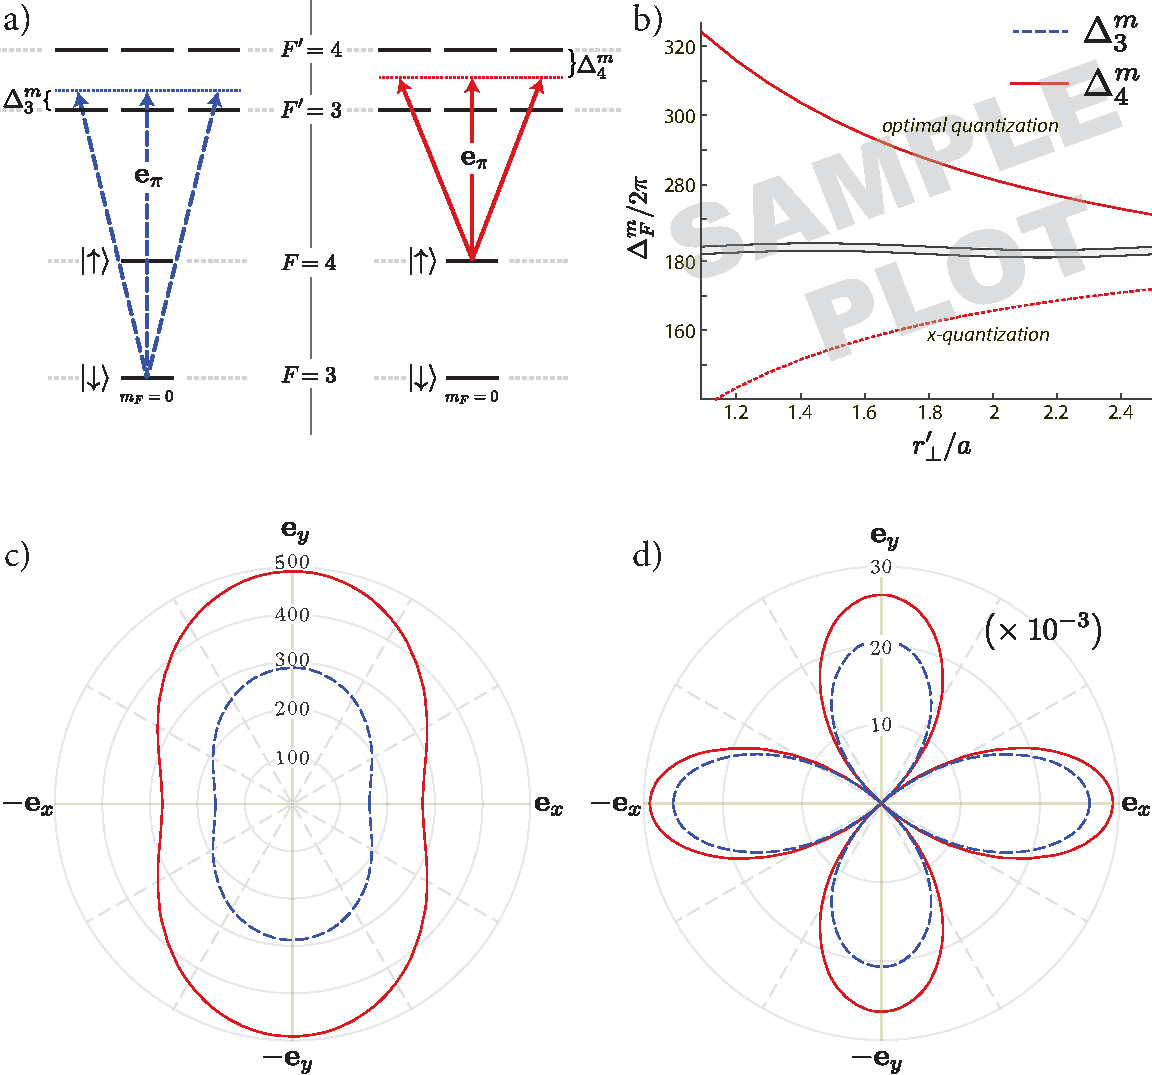
\includegraphics[scale=0.75]{./Figs/Fig_MagicFrequencies}
%\begin{minipage}{.32\linewidth}
%\centering
%\subfloat[]{\label{fig:D1_magicfreqs44_transition}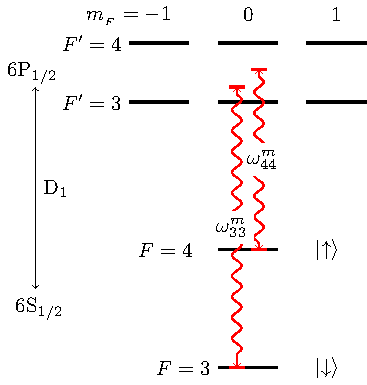
\includegraphics[scale=0.65]{./Figs/D1_magicfreqs44_transition}}
%\end{minipage}
%\begin{minipage}{.32\linewidth}
%\centering
%\subfloat[]{\label{fig:domega_magic12_q_NA2500_r1d8a}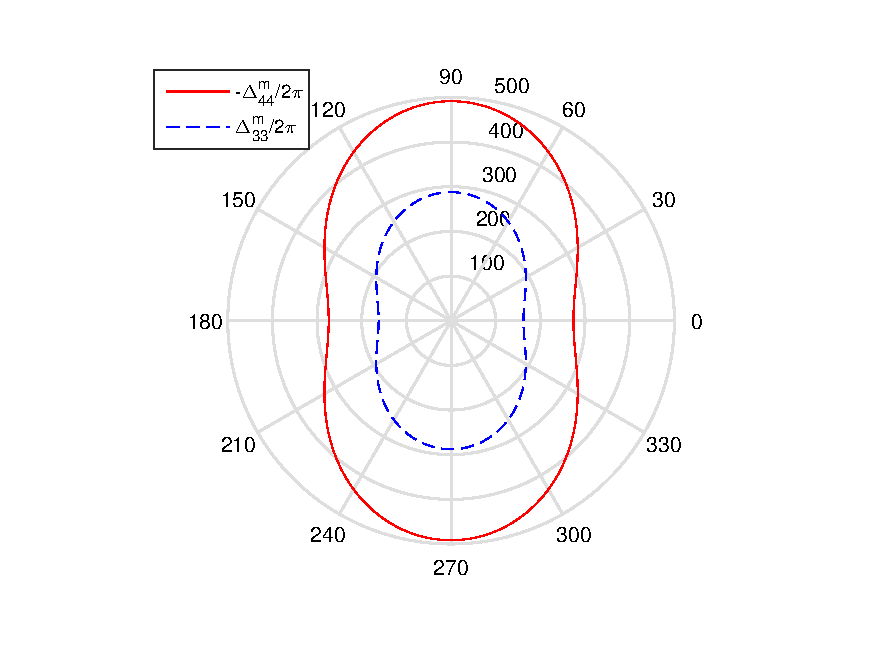
\includegraphics[scale=0.4]{./Figs/domega_magic12_q_NA2500_r1d8a}}
%\end{minipage}
%\begin{minipage}{.32\linewidth}
%\centering
%\subfloat[]{\label{fig:kappa_q_D1_xyplane_NA2500_r1d8a_m44}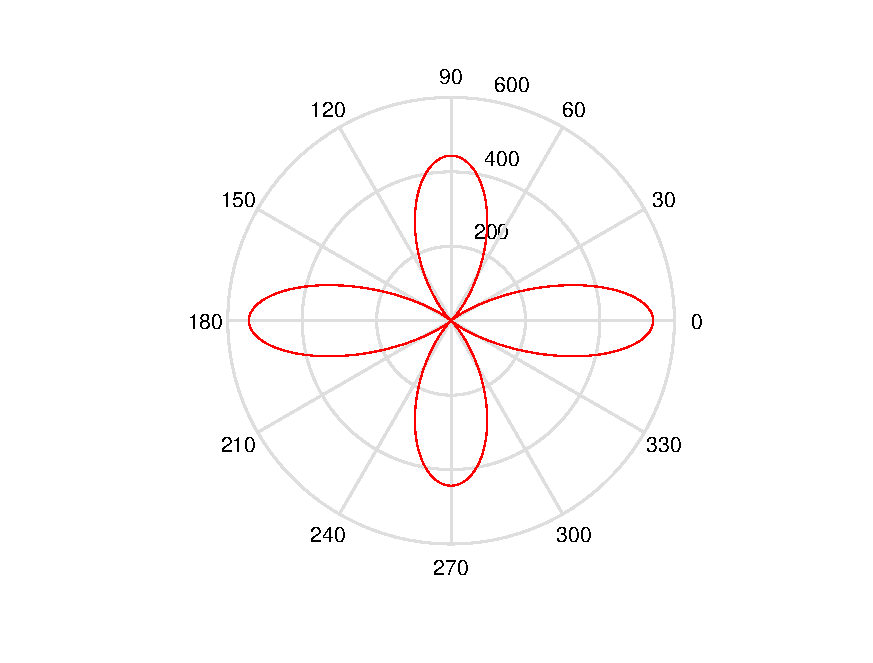
\includegraphics[scale=0.4]{./Figs/kappa_q_D1_xyplane_NA2500_r1d8a_m44}}
%\end{minipage}
\caption{Atom-light interface using the clock states of $^{133}$Cs.  
(a) Energy level structure for atoms probed with one of two magic frequencies on the D1-line. 
(b) Magic detuning, $\Delta^m_{F}/2\pi \equiv (\omega_{0} - \magic{F})/2\pi$, as the atoms are trapped further from the nanofiber shown for two contrasting quantization axes. 
(c) Magnitude of the magic detunings, $|\Delta^m_{F}|/2\pi$, and (d) dimensionless rotation angle $\chieff$ for an atom trapped on the \emph{x}-axis at $ r'\!_\perp=1.8a $ as the quantization axis, \erf{Eq::QuantizationAxis}, is varied in the $xy$-plane. }\label{Fig::CouplingStrength}
\end{figure}
%=============================================



The remaining QND interaction Hamiltonian is
	\begin{equation} \label{Eq::FaradayHam}
		\hat{H}_{J_3} = \hbar \chieff \jz \hat{S}_1(t),
	\end{equation}
where the rotation angle on the Poincar\'{e} sphere at the magic wavelength is,
\begin{equation}\label{eq:chiJ3}
\chieff = \big( \chi_{H, \uparrow} - \chi_{V,\uparrow} \big) - \big(\chi_{H,\downarrow} - \chi_{V,\downarrow} \big) = 2(\chi_{H, \uparrow}-\chi_{H, \downarrow}).
\end{equation}
In the standard way, squeezing the uncertainty in $\jz$ by QND measurement can be generated by preparing the atoms in a SCS along $\jx$, passing a probe prepared along $\hat{S}_2$ with photon flux $\dot{N}_L$, and continuously monitoring the $S_3$-component of the guided light in a polarimeter. The measurement strength,
	\begin{align} \label{Eq::MeasurementStrength}
		\kappa \equiv |\chieff|^2 \dot{N}_L, 
	\end{align}
with $\chieff$ given in Eq.~\eqref{eq:chiJ3}, quantifies the rate at which conditional projection noise is reduced. 
%\comment{Is this right? Where is the area of the input mode?}.  
In the absence of any decoherence, such a QND measurement for integration time $T$ squeezes the initial uncertainty in $J_3$ according to $(\Delta J_3^2)_{\rm out}= (\Delta J_3^2)_{\rm in}/(1+r)$, where
	\begin{equation}
		r = \kappa T  (\Delta J_3^2)_{\inp}
	\end{equation}
is the integrated measurement strength \cite{hammerer_quantum_2010, baragiola_three-dimensional_2014}.

%As discussed in Sec. \ref{Sec::AtomNumberMeasurement}, the  operator $\hat{\mathcal{M}}$ describes an integrated homodyne measurement of the anti-diagonal $X_L$-quadrature [\erf{Eq::Xquad}], 
%	\begin{align} \label{Eq::OutputS3Squeeze}
%		\hat{\mathcal{M}} & = \sqrt{\dot{N}_L/2} \big( \hat{X}_L^{\rm in} \error{\pm} \sqrt{\kappa/2} \hat{J}^\inp_z \big),
%	\end{align}
%where the input polarization mode plays the role of the local oscillator  \cite{vasilyev_quantum_2012,baragiola_three-dimensional_2014}. In the absence of decoherence the measurement is QND with finite resolution set by the inherent shot noise on the detector. The conditional variance is squeezed according to \cite{}
%	\begin{align} \label{Eq::IdealSqueezing}
%		\big(\Delta J_z^\out \big)^2 = \big( \Delta J_z^\inp \big)^2 \frac{1}{1+r},
%	\end{align}
%with collective measurement strength
%	\begin{align} \label{Eq::MeasurementStrength}
%		r \equiv \frac{ \projnoise }{ \shotnoise } = \kappa t \big( \Delta J_z^\inp \big)^2,
%	\end{align}
%where $\projnoise = \kappa \big( \Delta J_z^\inp \big)^2$ and $\shotnoise = 1/t$ are the (rescaled) projection noise and shot noise, respectively, for the integrated measurement in \erf{Eq::OutputS3Squeeze}. Significant spin squeezing is produced only when the projection noise is highly resolved over the shot noise.  


The strength of the birefringent interaction and thus the degree of achievable squeezing depend on the quantization axis that defines the clock state with projection $M=0$.  
We obtain an compact expression for the coupling strength in \erf{Eq::FaradayHam}, $\chieff$, using the irreducible tensor decomposition of the atomic polarizability, \erf{Eq::PolarizabilityIrrep}.  
Let $\{\mathbf{e}_1,\mathbf{e}_2, \mathbf{e}_\pi\}$ define a Cartesian basis.  Because of the azimuthal symmetry of clock state around the $\qaxis$-axis, the polarizability tensor is diagonal in that basis.  
Noting that $\langle F,0 | \hat{F}_{\pi}^2| F,0 \rangle =0$ and $\langle F,0 | \hat{F}_{1}^2| F,0 \rangle = \langle F,0 | \hat{F}_{2}^2| F,0 \rangle = \langle F,0 | \hat{\mathbf{F}}^2| F,0 \rangle /2 =F(F+1)/2$, it follows that the expectation value of the irreducible rank-2 component of the atomic polarizability is
	\begin{align} \label{Eq::CouplingAngleMagic}
		\langle F,0 | \poltens \phantom{}^{(2)}| F,0 \rangle  %= -\frac{\sigma_0}{8\pi k_0} F(F+1) \left( \frac{\unittens - 3\mathbf{e}_\pi \mathbf{e}_\pi}{6}  \right) \sum_{F'} C^{(2)}_{J'FF'}\frac{\Gamma}{ 2 \Delta_{FF'}}, \\
		= \sum_{F'} \alpha_0(F,F') C^{(2)}_{FF'} \frac{F(F+1)}{6} \Big( \unittens - 3\qaxis \otimes \qaxis \Big).
	\end{align}
The combined scalar and tensor light shifts yield a coupling strength, \erf{Eq::ClockCouplingStrength},
	\begin{align}
		\chi_{p,F} %&  = n_g \sigma_0 \sum_{F'}  \left\{C^{(0)}_{J'FF'}\left|\mathbf{u}_p(\br'_\perp)\right|^2+ C^{(2)}_{J'FF'} \frac{F(F+1)}{6}\left[\left|\mathbf{u}_p(\br'_\perp)\right|^2- 3 \left|\mathbf{e}_\pi \cdot \mathbf{u}_p(\br'_\perp)\right|^2 \right]\right\}   \frac{\Gamma}{4 \Delta_{FF'}} \nonumber  \\
		&  = n_g \sigma_0 \big(  a_{F} \left|\mathbf{u}_p(\br'_\perp)\right|^2 \error{-} b_{F} \left|\mathbf{e}_\pi \cdot \mathbf{u}_p(\br'_\perp)\right|^2 \big), \label{Eq::ClockStateCoupling}
	\end{align}
with coefficients that depend on detunings and atomic structure,
	\begin{align}
		%a_F &= \sum_{F'}  C^{(0)}_{J'FF'} \frac{\Gamma}{4 \Delta_{FF'}},\\
		%b_F &= \frac{F(F+1)}{6}\sum_{F'} C^{(2)}_{J'FF'}  \frac{\Gamma}{4 \Delta_{FF'}}.
		a_F &= \sum_{F'}  \Big(C^{(0)}_{FF'} + \frac{F(F+1)}{6} C^{(2)}_{FF'} \Big) \frac{\Gamma}{4 \Delta_{FF'}},\\
		b_F &= \frac{F(F+1)}{2}\sum_{F'} C^{(2)}_{FF'}  \frac{\Gamma}{4 \Delta_{FF'}}.
	\end{align}
\comment{Should there be $ C^{(2)}_{J'FF'} $? Should the $ \ket{\uparrow} $ and $ \ket{\downarrow} $ terms have different signs? Qi's formulas are shown below:
\begin{align}
		a_F &= \sum_{F'}  \Big(C^{(0)}_{FF'} + \frac{F(F+1)}{6} C^{(2)}_{FF'} \Big) \frac{(-1)^F\Gamma}{2 \Delta_{FF'}},\\
		b_F &= \frac{F(F+1)}{2}\sum_{F'} C^{(2)}_{FF'}  \frac{(-1)^F\Gamma}{2 \Delta_{FF'}}.
	\end{align}}

Birefringence arises from two effects.  
The first captures the effect of the anisotropy of the intensity of the $H$ and $V$ modes.  
Additionally, birefringence arises the tensor atomic response, which depends on $\mathbf{e}_\pi$ relative to the mode polarization. 
We write the effective rotation angle in the Hamiltonian, \erf{Eq::FaradayHam}, as
	\begin{align} \label{Eq::chieff}
		\chieff = - \frac{\sigma_0}{A_{J_3}} \frac{\Gamma}{ 2 \Delta_{J_3}},
	\end{align}
with an ``effective detuning" set by the magic-wavelength condition,
	\begin{align} \label{Eq::SqueezingEffectiveDetuning}
		 \Delta_{J_3}^{-1} \equiv \frac{2}{\Gamma} (b_4 \error{+} b_3) =   \sum_{F'}  \left( C^{(2)}_{\error{4F'}}\frac{10}{\Delta_{4F'}} -  C^{(2)}_{\error{3F'}}\frac{6}{ \Delta_{3F'} } \right),
	\end{align}
and an effective area given by \comment{(need to find a consistent way to use $ \br' $, $ \br'\!_\perp $ and $ r'\!_\perp $ for field components)}
	\begin{align} \label{Eq::SqueezingModeArea}
		A_{J_3}^{-1} & = n_g \frac{ |\mathbf{e}_\pi \cdot \mathbf{u}_H(\br'_\perp) |^2 |\mathbf{u}_V(\br'_\perp)|^2 - |\mathbf{e}_\pi \cdot \mathbf{u}_V(\br'_\perp)|^2 |\mathbf{u}_H(\br'_\perp)|^2}{ |\mathbf{u}_H(\br'_\perp)|^2 + |\mathbf{u}_V(\br'_\perp)|^2 } 
	\end{align}	
The quantization axis that maximizes $\chieff$ is that which minimizes $A_{J_3}$ at a given magic detuning.  

Their additional dependence on distance from the nanofiber is plotted in \frf{Fig::CouplingStrength}(c) for several choices of quantization axis. 
Since the $z$-component of the guided modes is $90^\circ$ out-of-phase with the transverse components, the quantization axis maximizing the atom-light coupling is specified by an angle in the transverse \emph{xy}-plane, 
	\begin{align} \label{Eq::QuantizationAxis}
		\qaxis = \cos \phi_\pi \mbf{e}_x + \sin \phi_\pi \mbf{e}_y.
	\end{align}
The dependence of the magic detunings on quantization axis is shown in \frf{Fig::CouplingStrength}(b) for atoms trapped at a typical distance of $r_\perp'=1.8a$ on the $x$-axis. 
In typical operating regimes, the magic frequencies are hundreds of MHz from resonance with either excited state, placing the interaction in the off-resonant, dispersive regime.
Finally, in \frf{Fig::CouplingStrength}(\comment{b}) we show the variation in $\chieff$ as a function of $\qaxis$.  
This suggests that, based solely on the strength of the coherent interaction, the $x$-axis serves as the optimal quantization axis.
As we see in the next section, the optimal quantization axis is significantly modified when decoherence due to optimal pumping is included. 
%The anisotropy of $\chieff$ results from several geometric factors, including the dependence of effective mode area $A_{J_3}$, \erf{Eq::SqueezingModeArea}, plotted in \frf{fig:phiq_optimal_NA500to5000_rp}, on $\mathbf{e}_\pi$. In addition, the tensor atomic response influences the value of the magic wavelength according to \erf{Eq::MagicWavelengthCondition}. 
 


	%====== SUBSECTION: Including optical pumping ======%
	\subsection{Decoherence due to optical pumping}

The treatment above considers an idealized QND interaction. The coupling of the atoms to the probe will always be accompanied by photon scattering into modes other than the forward scattered guided mode.  
This results in optical pumping that destroys the entanglement associated with spin squeezing.  
In addition it reduces the metrologically useful signal.  The maximum achievable meteorologically relevant squeezing is determined by the balance of this decoherence with the QND measurement. 

We fully model this based on a first-principles stochastic master equation (SME)~\cite{baragiola_three-dimensional_2014},
	\begin{align} \label{Eq::SME}
		d \hat{\rho} = s\sqrt{\frac{\kappa}{4}} \mathcal{H}[\hat{\rho}] dW + \frac{\kappa}{4} \mathcal{L}[\hat{\rho}] dt + \sum_n \mathcal{D}_n [\hat{\rho}] dt,
	\end{align}
where $s = {\rm sign}(\kappa)$ and $\hat{\rho}$ is the collective atomic state. 
The measurement strength $\kappa =|\chieff|^2 \dot{N}_L$ determines the amount of the spin squeezing in the absence of decoherence, \comment{\sout{\frf{fig:domega_magic12_q_NA2500_r1d8a} shows that the optimal choice of the quantization axis due solely to the coherent interaction is along the $x$-axis}}.  
The first two terms describe the QND measurement with strength $\kappa$ given in \erf{Eq::MeasurementStrength}. The conditional dynamics that result from the measurement are described by the superoperator
	\begin{align}
		\mathcal{H}[\hat{\rho}] = \jz \hat{\rho} + \hat{\rho} \jz - 2 \expt{\jz} \hat{\rho},
	\end{align}
where $dW$ is a stochastic Weiner increment satisfying $dW^2 = dt$, and ``measurement backaction" is given by the collective Lindblad map, 
	\begin{align}
		\mathcal{L}[\hat{\rho}] = - \smallfrac{1}{2}  \left(\hat{\rho}  \jz^2 + \jz^2 \hat{\rho}\right) + \jz \hat{\rho} \jz.
	\end{align}


The final term in \erf{Eq::SME} describes the effect of optical pumping acting locally on each atom along the nanofiber. 
Restricting to the two-dimensional subspace associated with the clock states for any given atom, the optical pumping map is governed by a standard master equation~\cite{deutsch_quantum_2010}.  
The action on the $n^{th}$ atom is
	\begin{align}
		\mathcal{D}_n[\hat{\rho}] =  \sum_{F=3,4} \Big\{& -\frac{\gamma_{F}}{2} \big[ \hat{\rho} (\op{F,0}{F,0})^{(n)} + (\op{F,0}{F,0})^{(n)}\hat{\rho} \big)]\\
		&+  \sum_{\tilde{F} =3,4}  \gamma_{F \rightarrow \tilde{F}}(\op{\tilde{F},0}{F,0})^{(n)} \hat{\rho}(\op{F,0}{\tilde{F},0})^{(n)} \Big\}.\nonumber
	\end{align}
Here, $\gamma_{F}$ is the total rate of photon scattering by atoms in the clock state $\ket{F,0}$, defined by
	\begin{equation}
		\gamma_{F}=- \frac{2}{\hbar} \Im \big[ \bra{F,0} \hat{H}_{\rm eff}\ket{F,0} \big] ,
	\end{equation}
%\comment{(Use Green's function here)} 
where $\hat{H}_\eff$ is the effective non-Hermitian light-shift Hamiltonian, \erf{Eq::LightShiftHam}, that accounts for the imaginary part of the atomic polarizability, $\charpol \rightarrow -(\sigma_0/8\pi k_0) \Gamma/(\Delta_{FF'}\comment{+}i\Gamma/2)$. 
The rates of optical pumping between the clock states, $\ket{F,0} \rightarrow \ket{\tilde{F},0}$, are
	\begin{equation}
		\gamma_{F \rightarrow \tilde{F} } =\big| \bra{F,0} \hat{W}_\pi \ket{\tilde{F},0} \big|^2,
	\end{equation}
where $\hat{W}_\pi$ is the Lindbald jump-operator associated with absorption of the probe photon followed by spontaneous emission of a $\pi$-polarized photon.  
These rates can be expressed in terms of the imaginary part of the polarizability tensor using \erf{Eq::Polarizability},
	\begin{align}
		\gamma_F &=\dot{N}_L  \sum_{F'} \sigma (\Delta_{FF'} ) \mathbf{u}^*_\inp(\br')\cdot \bra{F,0} \hat{\tensor{\mbf{A}}}(F,F') \ket{F,0}  \cdot \mathbf{u}_\inp(\br'), \\
		\gamma_{F \rightarrow \tilde{F}}&=  \dot{N}_L  \sum_{F'} \sigma (\Delta_{FF'}) \big| \mathbf{e}_\pi\cdot \bra{\tilde{F},0} \hat{\tensor{\mbf{A}}}(F,F') \ket{F,0}  \cdot \mathbf{u}_\inp(\br') \big|^2 ,
	\end{align}
where $ \sigma (\Delta_{FF'} )  = \sigma_0 \Gamma^2/4\Delta^2_{FF'}$ is the the scattering cross section at the probe detuning. When expressed in terms of Pauli operators on the pseudo-spin-$\half$ of the clock states,
	\begin{align} \label{Eq::OpticalPumpingMapSchr}
		\mathcal{D}_n [\hat{\rho}] 
				=& - \bigg( \frac{2(\gammau+ \gammad) - \gammauu - \gammadd}{4} \bigg) \hat{\rho} - \frac{ \gammau - \gammad - \gammauu + \gammadd }{4} \big( \hat{\sigma}_3^{(n)} \hat{\rho}+ \hat{\rho} \hat{\sigma}_3^{(n)} \big) \nn \\
		&+ \frac{\gammauu+\gammadd}{4} \hat{\sigma}_ 3^{(n)}\hat{\rho} \hat{\sigma}_3^{(n)} + \gammaud  \hat{\sigma}_-^{(n)} \hat{\rho} \hat{\sigma}_+^{(n)} + \gammadu  \hat{\sigma}_+^{(n)} \hat{\rho} \hat{\sigma}_- ^{(n)}.   
	\end{align} 
	
There are three important features of this map that are not typical in a QND measurement for spin-$\half$ particles.  
First, the map is not trace preserving as atoms are pumped out of the clock states. 
Second, unequal rates of optical pumping for $\ket{\uparrow}$ and $\ket{\downarrow}$ will polarize the mean $\expt{\jz}$ towards a value different from that found in the QND measurement. 
Third, owing to the large ground hyperfine splitting, $F' \rightarrow F=3$ and $F' \rightarrow F=4$ photons are distinguishable, thus coherences between $\ket{\uparrow}$ and $\ket{\downarrow}$ are destroyed.

We calculate the squeezing parameter as a function of time based on the evolution of atomic correlation functions. We work in the Heisenberg picture where operators evolve according to the adjoint form of the SME in \erf{Eq::SME}.  This leads to the following stochastic equations of motion (see Appendix \ref{Appendix::OpticalPumping})\comment{(double check the definition of $ \gamma_{30} $ in Appendix B)},
	\begin{align} 
		&d \NA = -\gamma_{00} \NA  dt + 2\gamma_{03} \expt{\hat{J}_3} dt \label{Eq::NA}\\
		&d \expt{\hat{J}_3}  = s\sqrt{\kappa} \varz dW -\gamma_{33} \expt{\hat{J}_3}dt + \smallfrac{1}{2}\gamma_{30} \NA dt   \\
		&d \expt{\hat{J}_1}  = -\gamma_{11} \expt{\hat{J}_1} dt  \\
		&d \varz  = - \kappa \big(\varz\big)^2 dt- 2 \gamma_{33} \varz dt + \smallfrac{1}{4} \big( 2\gamma_{33}-\gamma_{00} \big) \NA dt + \smallfrac{1}{2} \big( \gamma_{03} - 2 \gamma_{30} \big) \expt{\hat{J}_3} dt   \label{Eq::varJz} 
	\end{align}
where the decay and feeding rates are given in \erf{Eq::DecayRates}.  
We have also defined $ \NA $ as the atom number in the clock state subspace.
The final term in \erf{Eq::varJz}, proportional to $\expt{\hat{J}_3}$ is typically negligible, since in most applications $\expt{\hat{J}_3} \ll \NA$.  
We retain this small correction since unbalanced optical pumping will act to polarize the atom.  
Because this term is stochastic, we  solve the equations numerically. 

%========= SQUEEZING DYNAMICS: \xi, variance, mean,  N_A =========
\begin{figure}
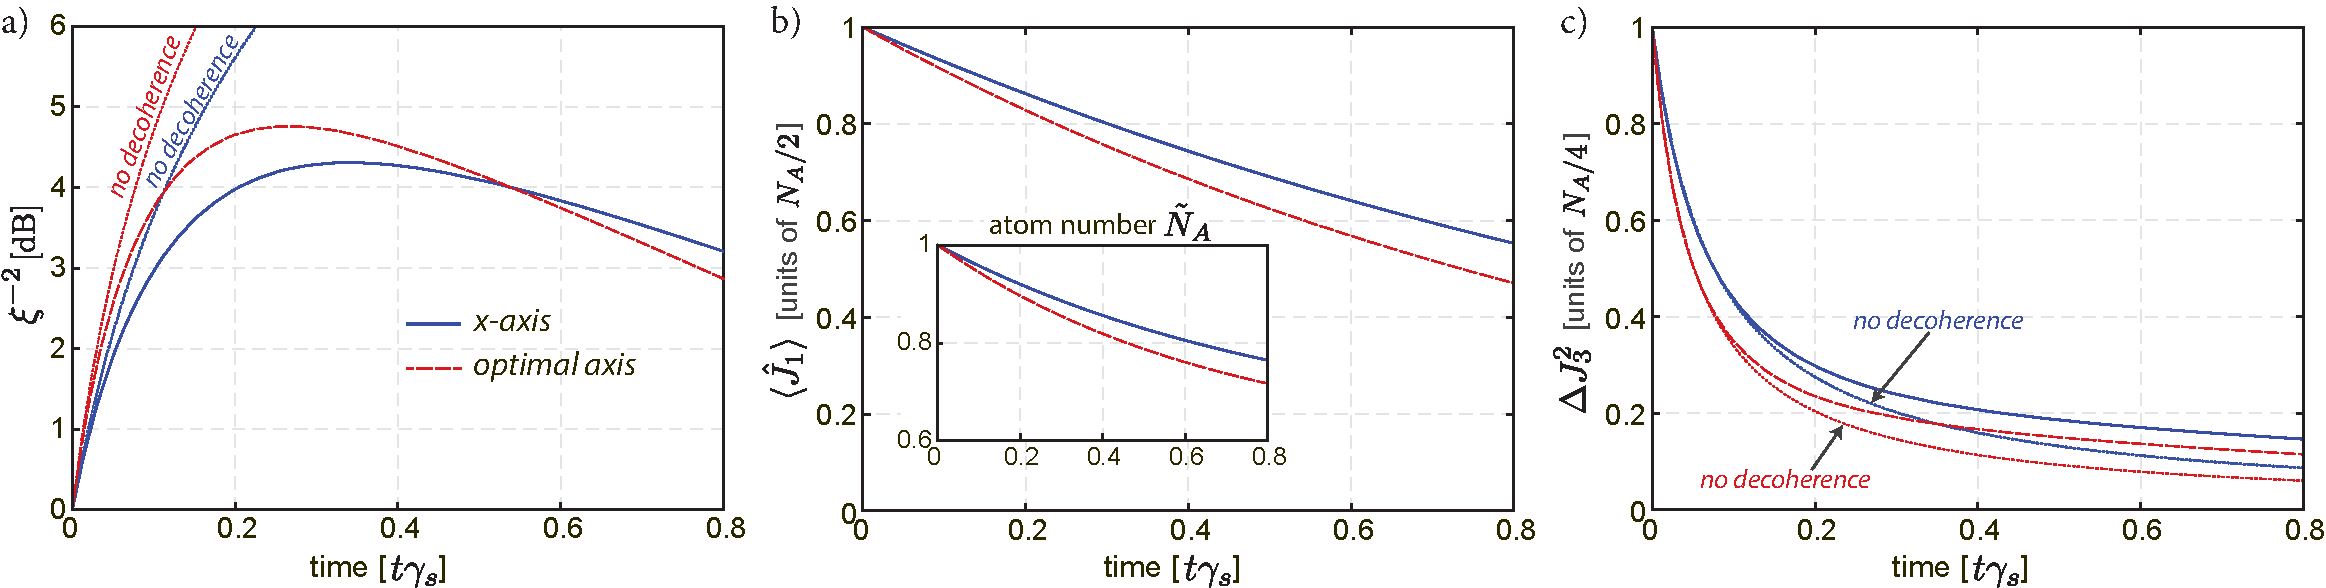
\includegraphics[scale=0.40]{./Figs/Fig_SqueezingDynamics}
%\begin{minipage}{.49\linewidth}
%\centering
%\subfloat[]{\label{fig:xit_qXoptimal_r1d8a_NA2500}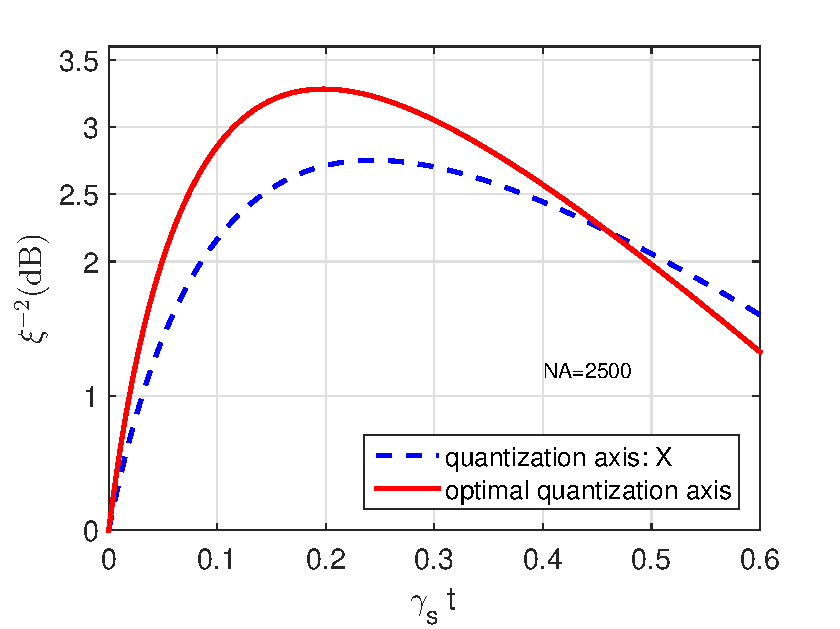
\includegraphics[scale=0.45]{./Figs/xit_qXoptimal_r1d8a_NA2500}}
%\end{minipage}
%\begin{minipage}{.49\linewidth}
%\centering
%\subfloat[]{\label{fig:DeltaJz2t_qXoptimal_r1d8a_NA2500}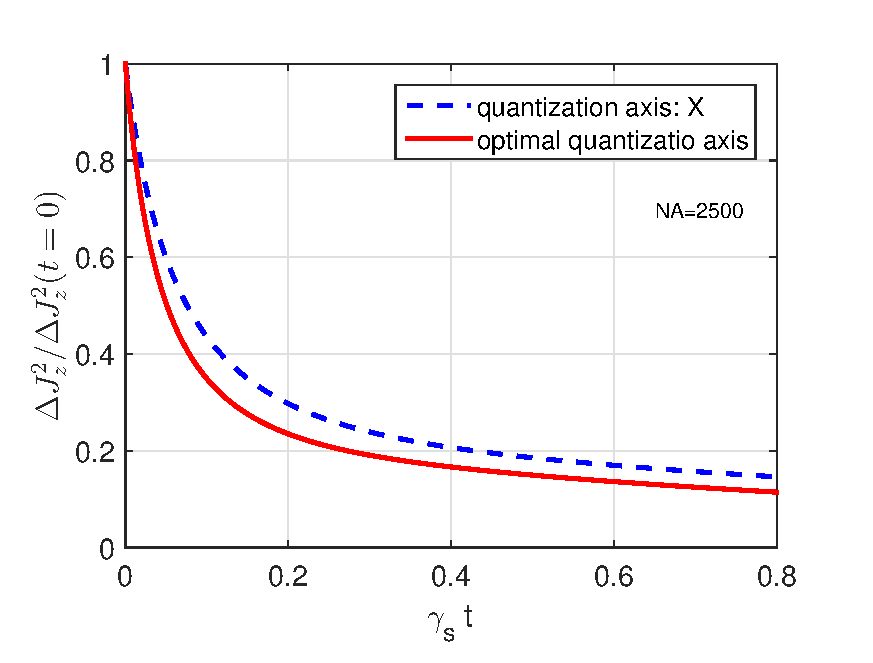
\includegraphics[scale=0.45]{./Figs/DeltaJz2t_qXoptimal_r1d8a_NA2500}}
%\end{minipage}
%\par\medskip
%\begin{minipage}{.49\linewidth}
%\centering
%\subfloat[]{\label{fig:Jxt_qXoptimal_r1d8a_NA2500}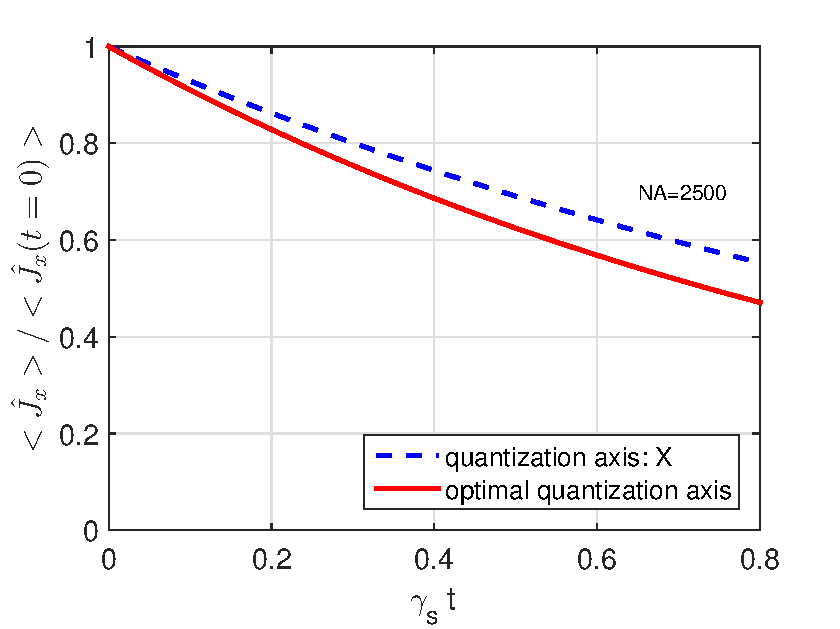
\includegraphics[scale=0.45]{./Figs/Jxt_qXoptimal_r1d8a_NA2500}}
%\end{minipage}
%\begin{minipage}{.49\linewidth}
%\centering
%\subfloat[]{\label{fig:NAt_qXoptimal_r1d8a_NA2500}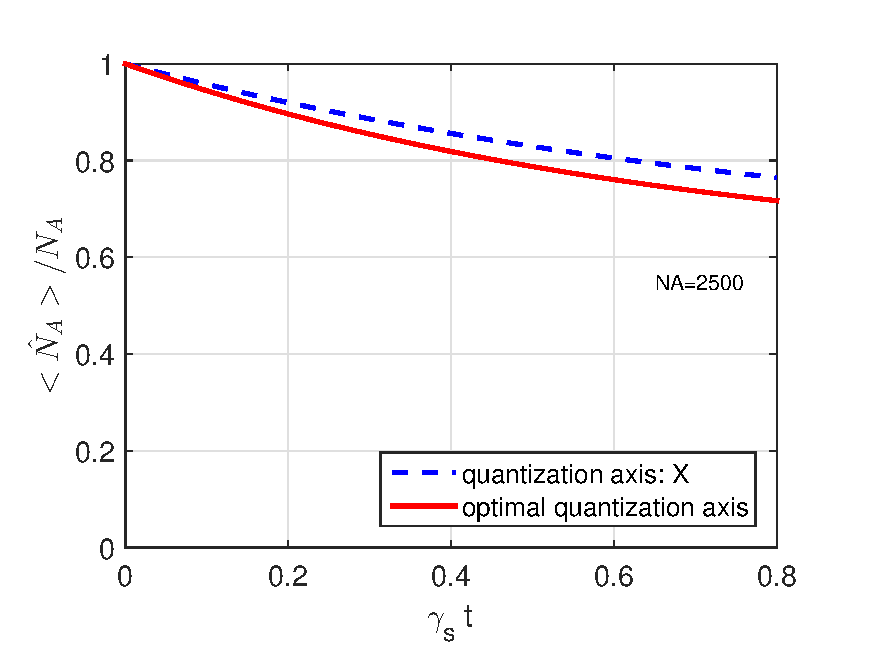
\includegraphics[scale=0.45]{./Figs/NAt_qXoptimal_r1d8a_NA2500}}
%\end{minipage}
\caption{Dynamics of spin squeezing on the clock states for $2500$ atoms trapped on the \emph{x}-axis at distance $ r'\!_\perp=1.8a$. 
The optimal quantization axis (red) is compared to quantization along the $x$-axis (blue). 
Solid lines indicate simulations with optical pumping and dashed lines without. 
(a) Metrological spin squeezing parameter $\xi^{2}$. 
(b) Conditional variance $\varz$. 
(c) Collective mean spin $\expt{\hat{J}_x}$ and decaying atom number $\NA$ (subplot). }\label{Fig::Squeezing_Dynamics}
\end{figure}
%================

To find the peak squeezing in the presence of optical pumping, we numerically integrate Eqs. (\ref{Eq::NA}--\ref{Eq::varJz}) and then calculate the squeezing parameter $\xi^2$ [\erf{Eq::SqueezingParameter}] as a function of time.
We choose here the magic frequency close to the $ F=4\leftrightarrow F'=4 $ transition, $ \magic{4} $ \comment{(need to make this notation consistent in plots)}, which is furthest from resonance with both excited hyperfine transitions.
Typical time dynamics are shown in \frf{Fig::Squeezing_Dynamics} for $2500$ atoms trapped on the \emph{x}-axis at a distance $r'\!_\perp=1.8a$ from the center of the nanofiber (as in \frf{}), where we operate the probe on the $\magic{4}$ magic detuning, and dimensionless time is scaled to the characteristic scattering rate, $\gamma_s \equiv (\sigma_0/A_{\rm in})(\Gamma/2 \Delta_\eff)^2 \dot{N}_L$.
We show the dynamics for two choices of quantization axis: (i) along the $x$-axis and (ii) along the numerically determined optimal axis, $\phi_\pi \approx 86^\circ$ in \erf{Eq::QuantizationAxis}. 
We begin with the dynamics of the squeezing parameter in \frf{fig:xit_qXoptimal_r1d8a_NA2500}. 
In the presence of optical pumping, peak squeezing is limited by the combined effects of decoherence on $\expt{\jx}$ and $\varz$, the constituent moments that determine $\xi^2$. 
The primary factor that limits metrological squeezing is the decay of the collective mean $\expt{\jx}$ \cite{baragiola_three-dimensional_2014}, plotted in (b). 
A scattered photon eliminates the initial coherence between $\ket{\uparrow}$ and $\ket{\downarrow}$ within a single atom, thus depolarizing the collective mean spin $\expt{\jx}$. 
Atoms optically pumped to magnetic sublevels outside of the clock subspace decay $\NA$, further reducing $\expt{\jx}$.
The QND squeezing of the conditional variance, $\varz$, competes with the noise injected by atoms that return to the clock subspace. 
An additional source of decoherence comes from the decay of the two-body correlations that lie at the heart of spin squeezing, as described by \erf{Eq::TwoBodyDecay}.
All of these effects are included in the equation for $\varz$, \erf{Eq::varJz}, whose dynamics are shown in (c). \comment{(Since we write the equation for $\expt{\hat{J}_3}$ and explicitly comment about its dynamics being stochastic, perhaps we should show it along with the others here. 
This would reveal only that it is small compared to $\NA$ and experiences deterministic polarization towards $\ket{\downarrow}$. We can give a sample and the averaged stochastic process for a fixed atom.)}

%========= FIGURE: Peak squeezing (\xi, measurement strength, scattering rates) =========
\begin{figure}
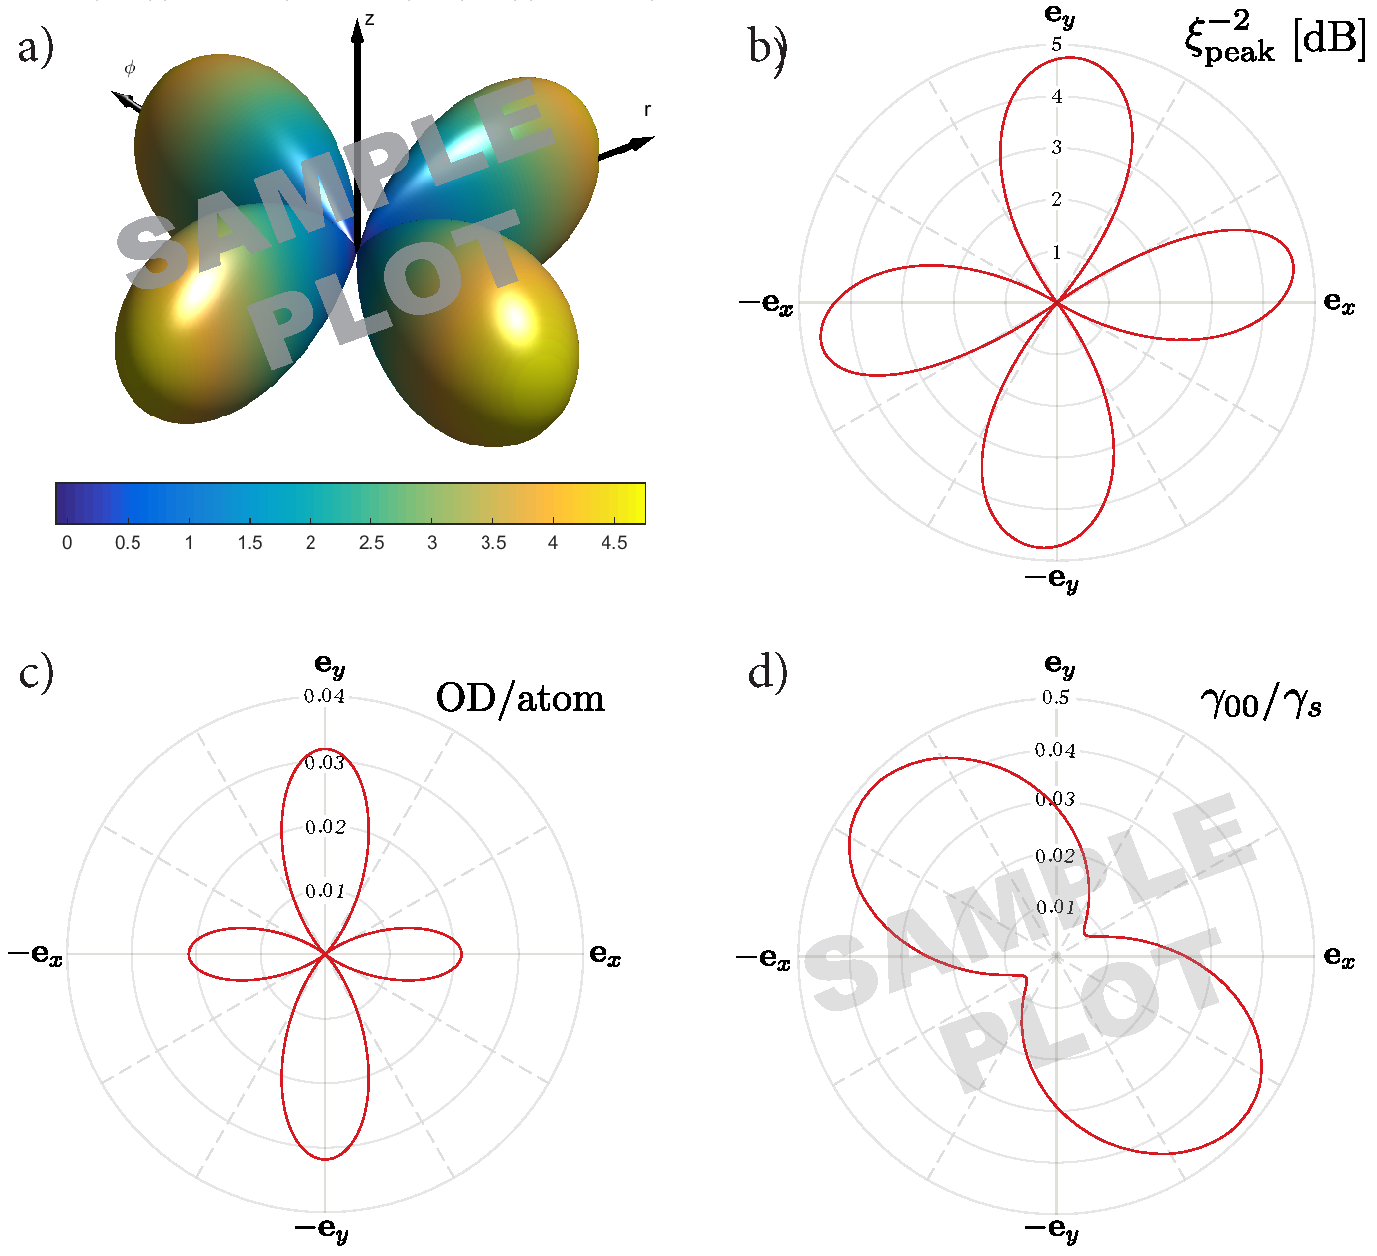
\includegraphics[scale=0.45]{./Figs/Fig_SqueezingQuantAxis}
%\begin{minipage}{.49\linewidth}
%\centering
%\subfloat[]{\label{fig:xi_q_D1_NA2500_r1d8a}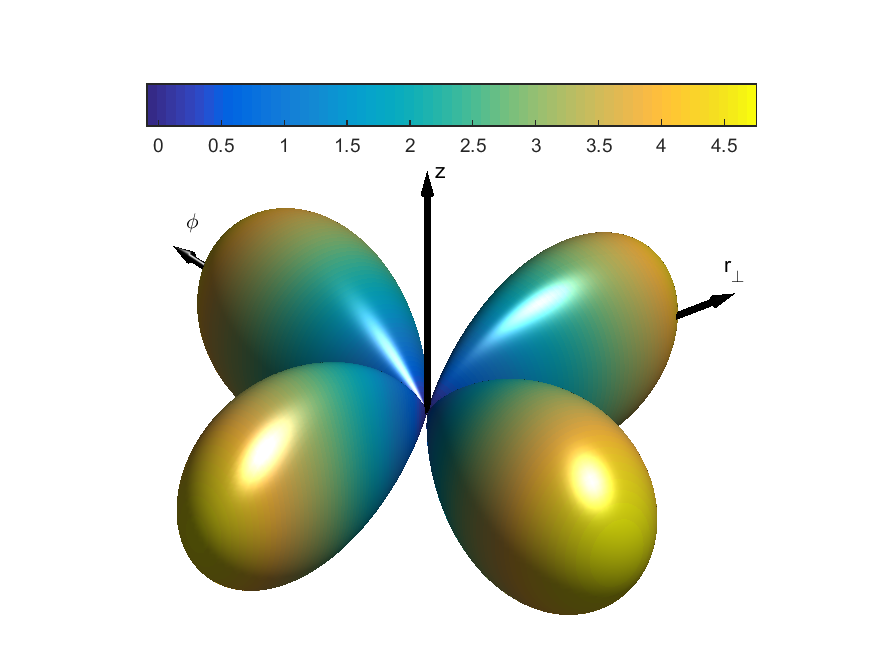
\includegraphics[scale=0.45]{./Figs/xi_q_D1_NA2500_r1d8a}}
%\end{minipage}
%\begin{minipage}{.49\linewidth}
%\centering
%\subfloat[]{\label{fig:ximax_q_D1_xyplane_NA2500_r1d8a}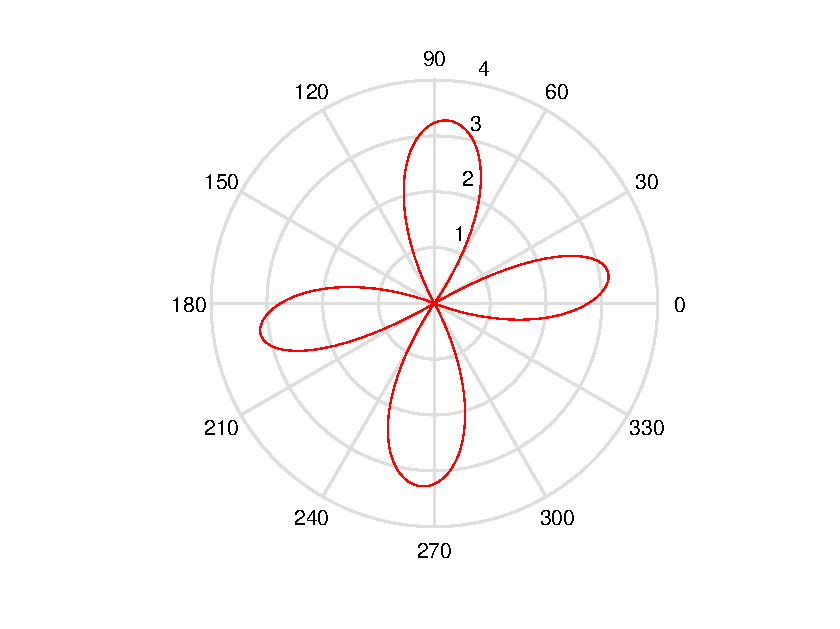
\includegraphics[scale=0.45]{./Figs/ximax_q_D1_xyplane_NA2500_r1d8a}}
%\end{minipage}
%\par\medskip
%\begin{minipage}{.32\linewidth}
%\centering
%\subfloat[]{\label{fig:OD_q_xyplane_r1d8a_m44}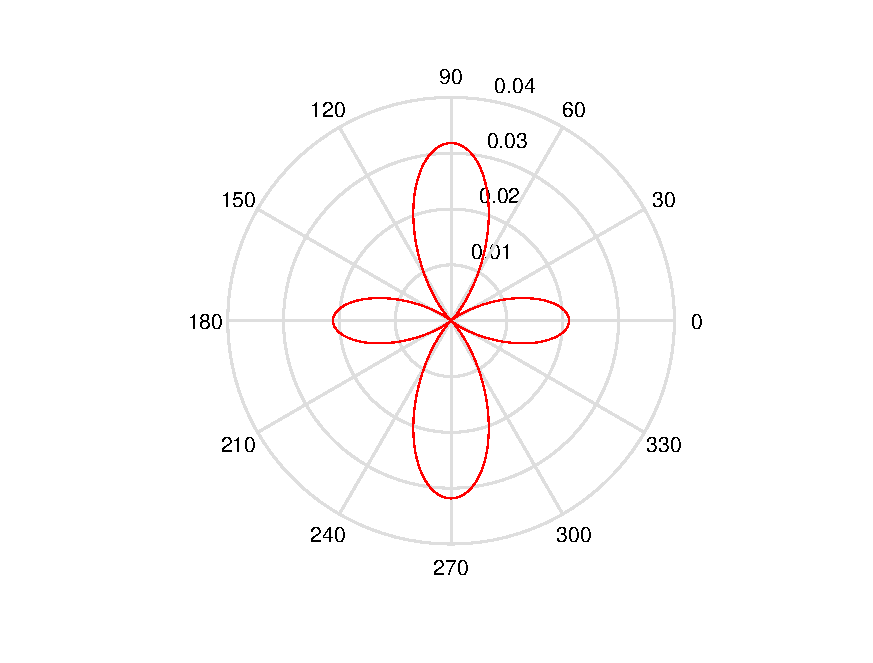
\includegraphics[scale=0.4]{./Figs/OD_q_xyplane_r1d8a_m44}}
%\end{minipage}
%\begin{minipage}{.32\linewidth}
%\centering
%\subfloat[]{\label{fig:gamma34togammas_q_D1_xyplane_NA2500_r1d8a_m44}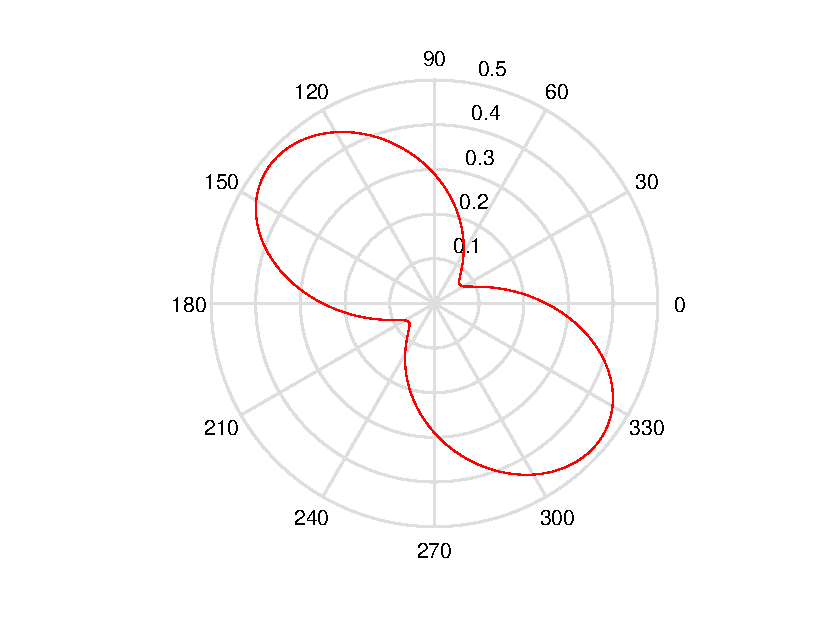
\includegraphics[scale=0.4]{./Figs/gamma34togammas_q_D1_xyplane_NA2500_r1d8a_m44}}
%\end{minipage}
%\begin{minipage}{.32\linewidth}
%\centering
%\subfloat[]{\label{fig:OD_optimal_rp}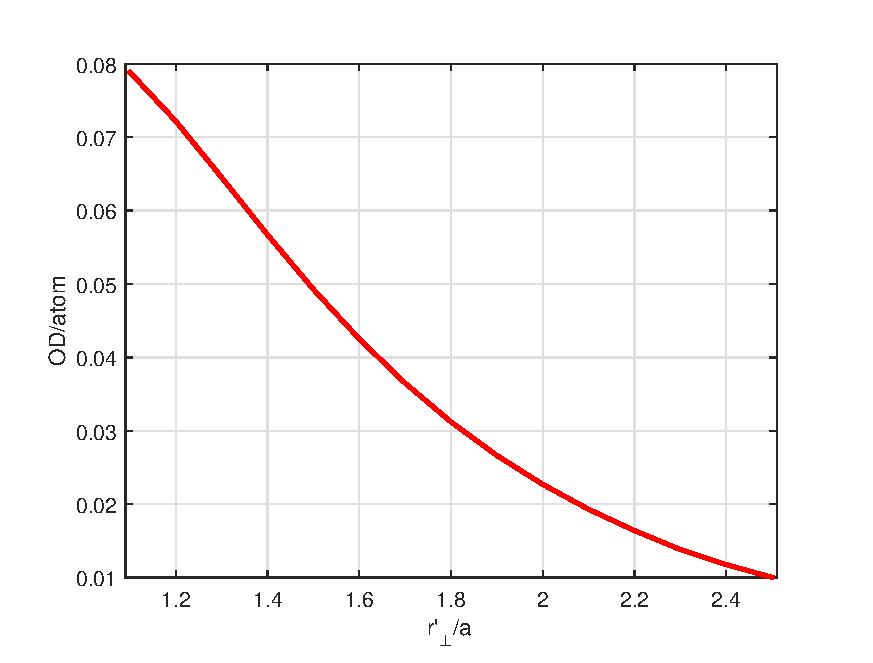
\includegraphics[scale=0.4]{./Figs/OD_optimal_rp}}
%\end{minipage}
\caption{Dependence of metrological squeezing on quantization axis, $\qaxis$, for $2500$ atoms trapped on the \emph{x}-axis at a distance $ r'\!_\perp=1.8a$. In (b--d) $\qaxis$ is confined to the \emph{xy}-plane where the optimal peak squeezing occurs.
(a--b) Peak squeezing for varying $\qaxis$. 
(c) OD/atom.
(d) Rates of atom loss, $\gamma_{00}$, and depolarization, $\gamma_{11}$. }\label{Fig::Squeezing_QuantizationAxis}
\end{figure}
%================

The choice of quantization axis $\qaxis$ along which the clock states are defined affects both the measurement strength and the relative rates of optical pumping. 
We plot peak squeezing for $\qaxis$ in the $xy$-plane in \frf{Fig::Squeezing_QuantizationAxis}(a).
With only $2500$ atoms at $r_\perp = 1.8a$, peak squeezing can be as large as \comment{4.7 dB} when the clock states are chosen along the optimal axis, $\qangle^{\rm opt} \approx 86^\circ$ in \erf{Eq::QuantizationAxis}\comment{(the same information has been maintained in the last paragraph)}. 
We gain insight into the balance between QND measurement and optical pumping by independent inspection of the measurement strength and decoherence rates. 
First, the rate of squeezing is determined by the OD/atom $=\sigma_0 A_{\rm in}/A_{J_3}^2$ (equivalent to the dimensionless measurement strength $\kappa/\gamma_s$), which peaks along the $y$-axis as seen in \frf{Fig::Squeezing_QuantizationAxis}(a). 
Along $y$, the OD/atom is about 50\% larger than along $x$-axis.
Second, from the fact that magic frequency, $\magic{4}$, lies nearly equidistant from $F'=3$ and $F'=4$, see \frf{Fig::CouplingStrength}(b)\comment{(in this paragraph, some figure labels seem to be misplaced or subfigures to be rearanged?)}, one might conclude that quantization along $y$-axis also provides more protection from decoherence. 
This conclusion is supported by \frf{Fig::Squeezing_QuantizationAxis}(c), where the rates of atom loss, $\gamma_{00}$, and of depolarization, $\gamma_{11}$, which appear in the equations of motion for the moments, Eqs. (\ref{Eq::NA}--\ref{Eq::varJz}), favor quantization in the first quadrant near the $y$-axis. 
In contrast, using the free-space trapping configuration, there is no difference to choose a quantization axis in any direction on the transverse plane due to the isotropy property of free space. 


The dispersive entangling interaction is based on the collective atomic coupling to the evanescent guided-mode fields, which decay exponentially away from the nanofiber surface. 
Thus the OD/atom increases as the atoms are trapped closer to the surface, as seen in \frf{Fig::Squeezing_Distance}(a). 
\error{Since $\varz$ is nonlinear in atom number} from Eq.~\eqref{Eq::varJz}, the optimal choice of quantization axis depends not only on $r_\perp$ but also weakly on the atom number, \frf{Fig::Squeezing_Distance}(b). 
At the optimal quantization axis, the strong dependence of peak achievable squeezing on distance from the fiber is as seen in \frf{Fig::Squeezing_Distance}(c)\comment{(also double check the labels in this paragraph)} along with the expected increase as more atoms contribute to the atom-light interface. 

Several effects limit the reliability of the simulations as $r_\perp \rightarrow a$. 
First, strong van der Waals interactions modify the light shifts and magic frequencies near the fiber surface \cite{lacroute_state-insensitive_2012}.
Second, the optical pumping model used here breaks down near the surface where the local density of states is significantly modified in the presence of the dielectric nanofiber \cite{le_kien_spontaneous_2005}. 
At distances \comment{$r_\perp > 1.5a$} the atoms' local environment is roughly that of unmodified vacuum and a free-space optical pumping model in \erf{Eq::OpticalPumpingMapSchr} suffices. 


%======= FIG: Scaling with atom number and distance =======
\begin{figure}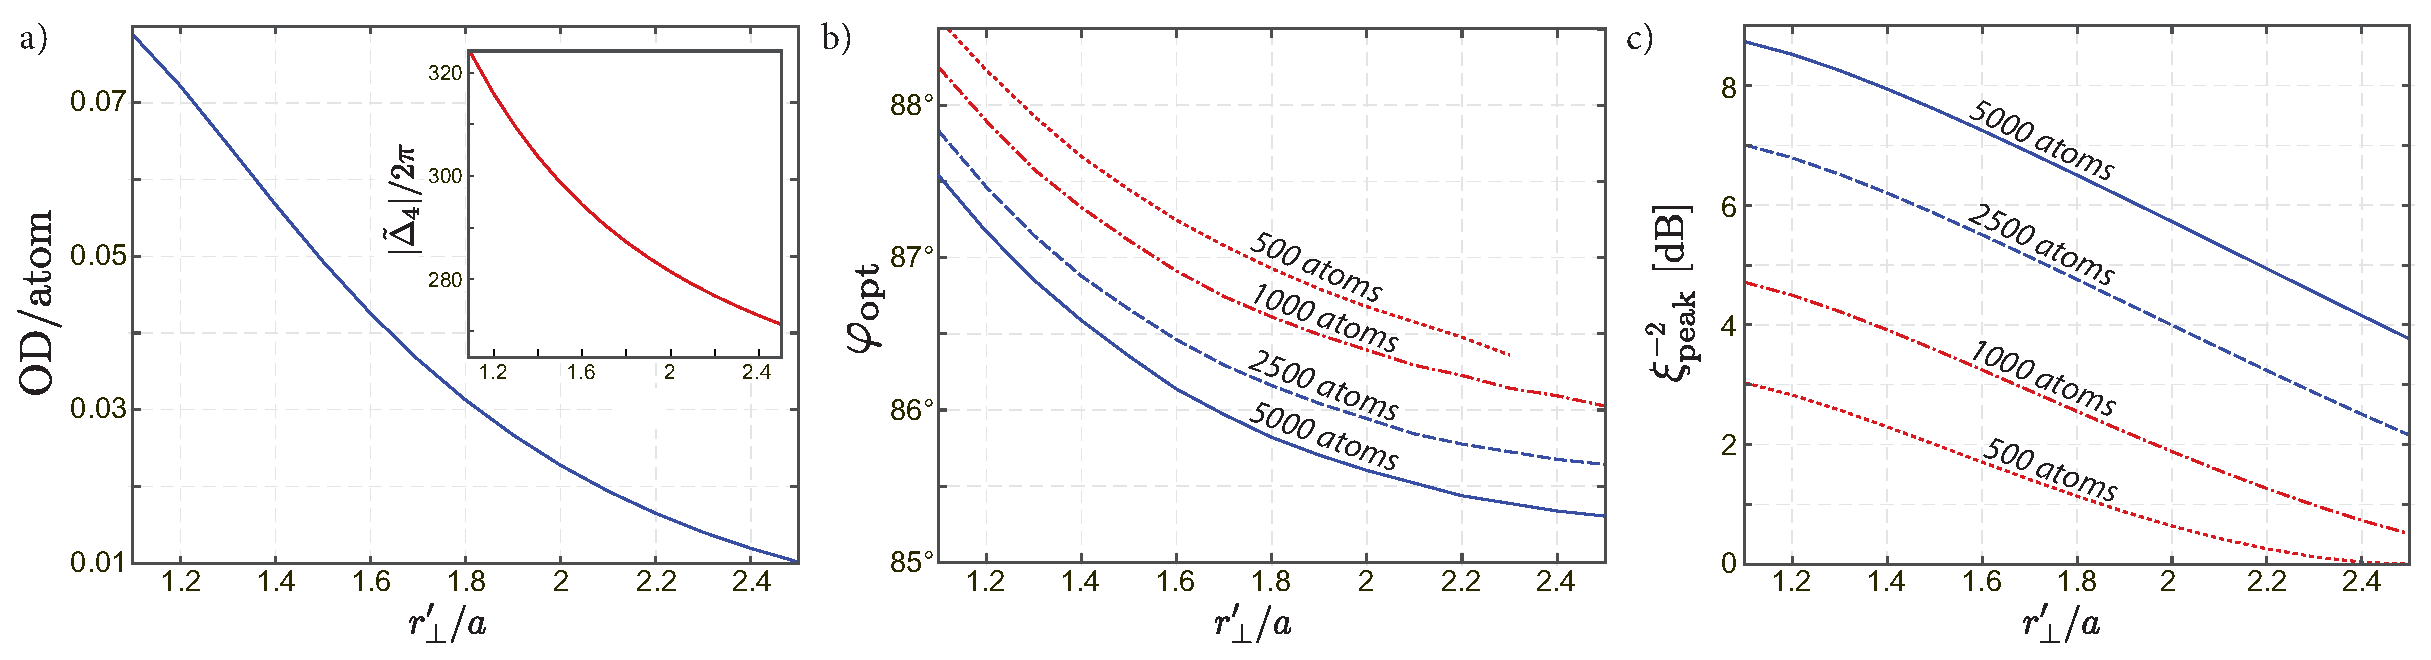
\includegraphics[scale=0.4]{./Figs/Fig_SqueezingDistance}
%\begin{minipage}{.49\linewidth}
%\centering
%\subfloat[]{\label{fig:phiq_optimal_NA500to5000_rp}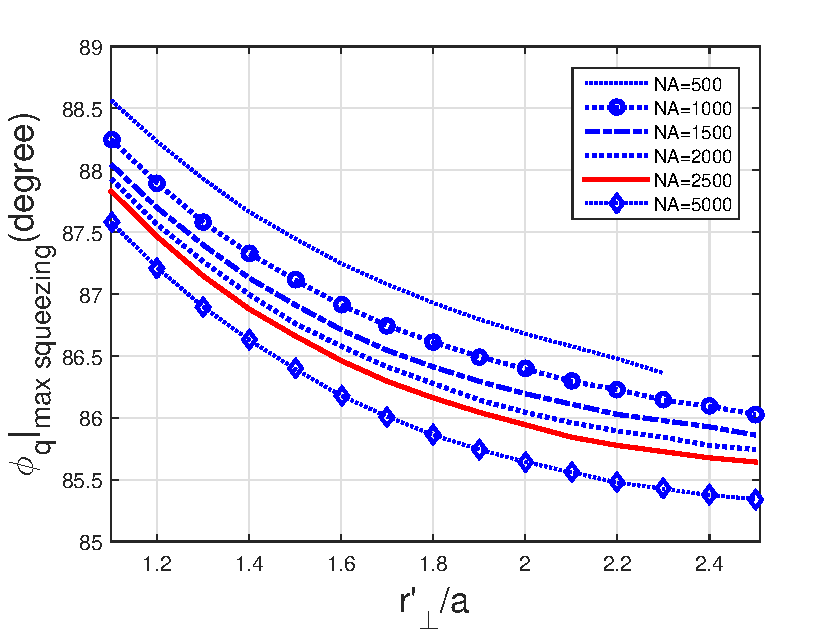
\includegraphics[scale=0.45]{./Figs/phiq_optimal_NA500to5000_rp}}
%\end{minipage}
%\begin{minipage}{.49\linewidth}
%\centering
%\subfloat[]{\label{fig:xi_optimal_NA500to5000_omega44}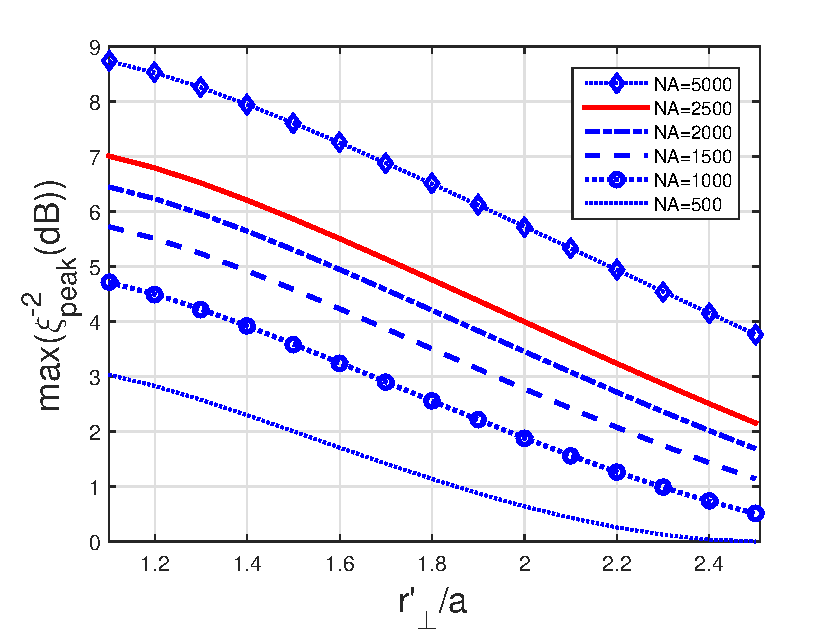
\includegraphics[scale=0.45]{./Figs/xi_optimal_NA500to5000_omega44}}
%\end{minipage}
%\par\medskip
%\begin{minipage}{.49\linewidth}
%\centering
%\subfloat[]{\label{fig:domega_magic44_qXYoptimal_rp}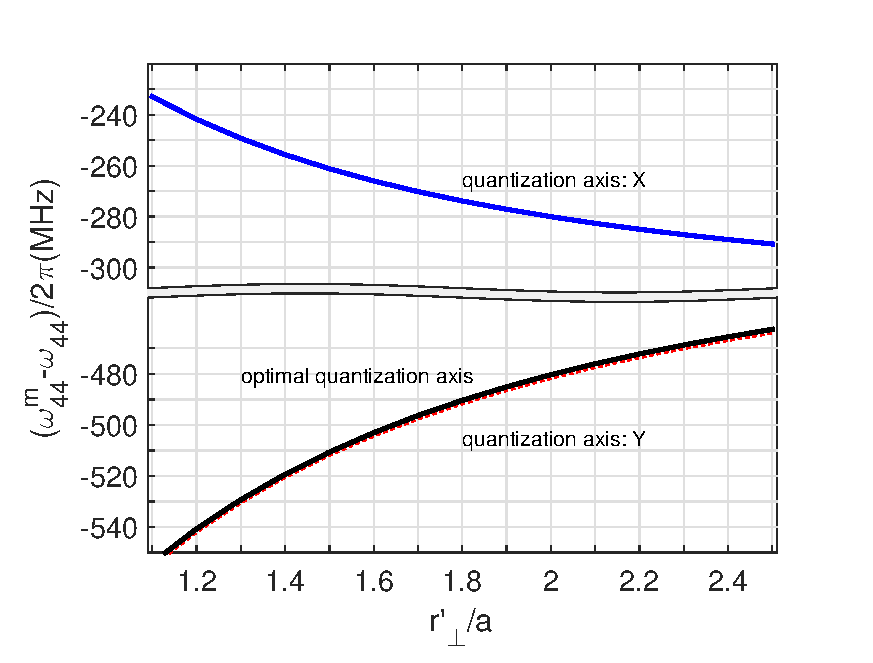
\includegraphics[scale=0.45]{./Figs/domega_magic44_qXYoptimal_rp}}
%\end{minipage}
%\begin{minipage}{.49\linewidth}
%\centering
%\subfloat[]{\label{fig:domega_magic33_qXYoptimal_rp}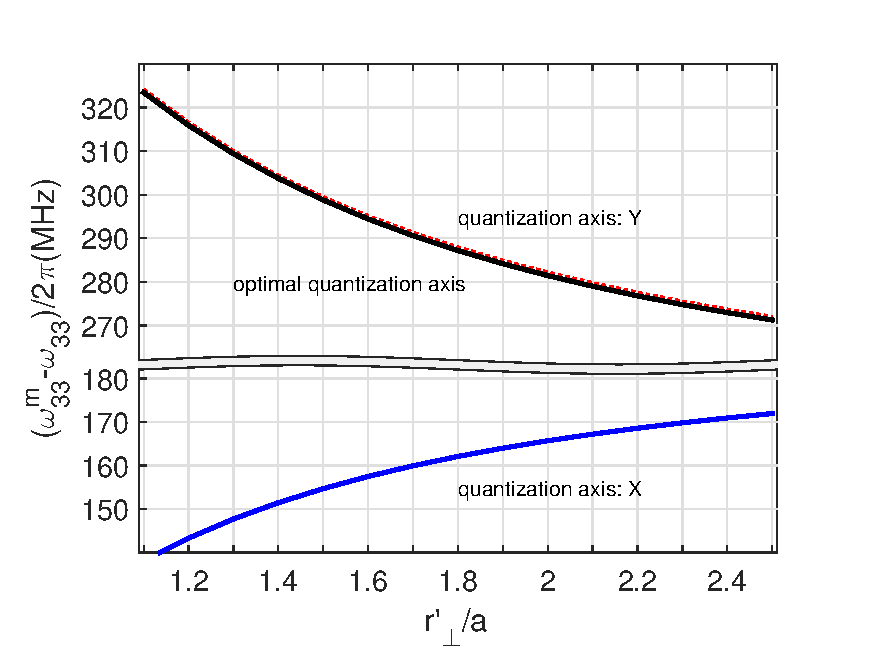
\includegraphics[scale=0.45]{./Figs/domega_magic33_qXYoptimal_rp}}
%\end{minipage}
\caption{Squeezing as a function of trapping distance $r_\perp$ and initial atom number $N_A$. (a) OD/atom. (b) Optimal quantization axis $\qaxis$. 
%The line is cut off when the squeezing effect is too weak to be observed ($ r'\!_\perp>2.3a $).
(c) Peak metrological squeezing at the optimal $\qaxis$.} \label{Fig::Squeezing_Distance}
\end{figure}
%================================


%====== SECTION: Summary and outlook ======%
\section{Conclusions and outlook}

Using the nanofiber geometry, $ \mathrm{OD}/\mathrm{atom}\sim 10^{-2} $ approaches that achieved for atomic ensembles trapped inside optical cavities of moderate finesse \cite{chen_conditional_2011}.  The ideal atom-light interaction is entirely symmetric along the nanofiber providing the foundation for long-range  correlations independent of distance between the atoms. As the light is entirely guided, fiber-couped atomic ensembles can be simply networked together for truly long-range entanglement generation and distribution. 

In contrast, for atoms trapped in free space, the atom-light coupling is typically orders of magnitude smaller, $ \mathrm{OD}/\mathrm{atom} \approx 10^{-5}$, requiring millions of atoms to achieve several dB of squeezing \cite{}.

Going beyond Gaussian squeezed states--how close are we at $\sim 4.7$ dB for 2500 atoms? Could we get there by using Leigh's method of state preparations to increase along with the benefits of the nanofiber to increase $\kappa$? What about different state preparations such as the stretched states, which have more favorable decoherence? 

\comment{ 
In their final discussion, Polzik et al. \cite{beguin_generation_2014} extrapolate their experiment to give numerical estimates of spin squeezing for 2500 atoms.  
They report 4.2 dB of spin squeezing when the noise channel is ``damping of hyperfine coherence due to photon scattering \change{(note--this is $\gamma_{33}$)}" and atom loss is neglected. 
}

Outside of a waveguide, cavity enhancement can produce drastic increases in atom-number detection, \cite{zhang_collective_2012}, spin squeezing \cite{bohnet_reduced_2014}, and....   
Strong coupling to the guided nanofiber modes can be further improved with nanofabricated cavities that, under EIT conditions, substantially slow the group velocity \cite{le_kien_intracavity_2009,wuttke_nanofiber_2012,nayak_optical_2014}.  Additional hybrid approaches \cite{hafezi_atomic_2012, yalla_cavity_2014}.  Coherent quantum control of atoms \cite{smith_quantum_2013-1}.  
Quantum sensing \cite{kumar_autler-townes_2015}.  Preparation of nonclassical light using collective dissipation \cite{gonzalez-tudela_deterministic_2015}.  
Optical memory (not quite quantum) \cite{sayrin_storage_2015, gouraud_demonstration_2015} Interaction with higher-order modes.  Optical switching using a single atom \cite{oshea_fiber-optical_2013} 

Optical pumping near the surface of a dielectric that modifies the local density of states, 

Initial state preparation can improve the precision of dispersive atom number measurements, 

Reaching the edge of Gaussian states?

More insights on the anisotropy of photonic waveguide and two-body correlations will be a future work.

\cite{scheel_directional_2015}
\comment{Any discussion of metallic nanowires?}

\comment{
OTHER FIGURES FOR ELSEWHERE IN PAPER \\
\emph{Figure}: Nanofiber schematic \\
\emph{Figure}: Phase shift \\
\emph{Figure}: Atom number resolution \\
\emph{Figure}: Atomic structure \\
a) clock-state level structure and $H,V$-transitions \\
b) magic wavelength (in detuning) as a function of quantization axis $\phi_Q$ in $x,y$-plane \\
c) magic wavelength (in detuning) as a function of distance from the fiber $r_\perp/a$ for fixed $\phi_Q$ 

}

%\begin{center}
%{\bf References}
%\end{center}

%\bibliography
%\bibliographystyle{amsplain}
\bibliographystyle{unsrt}
\bibliography{Nanofibers}
% \nocite{*}
%\ifwindows
%	\bibliography{F:/References/Archive/Archive}
%\else
%	\bibliography{/media/F/References/Archive/Archive}
%\fi

%=========== APPENDIX ===========%
\begin{appendix}	


%=========== APPENDIX: Nanofiber mode functions ===========%
\section{Guided-mode functions for the optical nanofiber} \label{Appendix::ModeFunctions}

Here we briefly review the guided-mode eigenfunctions for an optical nanofiber.  The nanofiber's distinguishing feature that the diameter is smaller than the operating wavelength of light has several consequences.  
First, a significant fraction of the transmitted power resides in evanescent fields that can extend well beyond the nanofiber's surface.  
This evanescent field is the tool with which atoms are trapped and manipulated by fiber-guided light.  
Second, the guided modes outside the taper region adiabatically transform through the fiber taper into the modes of the nanofiber without significant losses.  
Through this transformation, the guided fields acquire a large component along the fiber axis that is out of phase with the transverse components, which makes the nanofiber modes significantly different from the transverse plane waves or paraxial modes in free space.    

Here, we provide the fundamental HE$_{11}$ solutions to the homogeneous wave equation, \erf{Eq::WaveEquationSource} with $\tensor{\boldsymbol{\alpha}} = 0$, for a cylindrical nanofiber of radius $a$ and index of refraction given by \erf{Eq::IndexofRefraction}.  
At a given frequency, $\omega_0 = c k_0$, the magnitudes of the longitudinal and transverse wave vectors for a guided mode are related by $n^2 k_0^2 = \beta_0^2 + k_\perp^2$.  
The positive propagation constant, $\beta_0 \equiv \beta(\omega_0)$, is determined from the eigenvalue equation that results from enforcing physical boundary conditions at the fiber surface \cite{Yariv, Marcuse, Snyder and Love},
	\begin{align}
		\frac{J_0(ha)}{ha J_1(ha)} = - \frac{n_1^2+n_2^2}{2n_1^2} \frac{K'(qa)}{qa K_1(qa)} + \frac{1}{h^2 a^2} - \bigg[ \bigg(\frac{n_1^2 - n_2^2}{2 n_1^2} \frac{K'(qa)}{qa K_1(qa)} \bigg)^2  + \frac{\beta_0^2}{n^2_1 k^2} \bigg(\frac{1}{q^2a^2} + \frac{1}{h^2a^2} \bigg)^2 \bigg]^{1/2}.
	\end{align}
Inside the nanofiber the transverse wavevector is real, $k_\perp = q$, where $q=\sqrt{\beta_0^2- n_2^2k_0^2}$, and outside the nanofiber it is purely imaginary, $k_\perp = i h$, where $h=\sqrt{n_1^2 k_0^2 - \beta_0^2}$.  The vector eigenfunctions are expressed as $\mbf{f}_{\mu}(\br) = (2\pi)^{-1/2}\mbf{u}_{f,p}(\mbf{r}_\perp) e^{i f \beta_0 z}$, where the modes are indexed by frequency $\omega_0$, propagation direction $f = \pm$, and polarization $p$.

A relatively simple form for the guided-mode functions can be expressed in a cylindrical basis $(r_\perp, \phi, z)$ with longitudinal unit vector $\mathbf{e}_z$, oriented along the fiber axis.  
The transverse unit vectors are related to their fixed Cartesian counterparts via the relations
	\begin{align}
		\mathbf{e}_r     &= \mathbf{e}_x \cos \phi + \mathbf{e}_y \sin \phi, \\
		\mathbf{e}_\phi &= - \mathbf{e}_x \sin \phi + \mathbf{e}_y \cos \phi.
	\end{align}
The transverse profile for the quasicircular guided modes, $p = \pm$, is
	\begin{align} \label{Eq::QuasicircularModes}
		\mbf{u}_{f,\pm}(\mathbf{r}_\perp) = \big[\mathbf{e}_r u_r(r_\perp) \pm i \mathbf{e}_\phi u_\phi(r_\perp) +  i f \mathbf{e}_z  u_z(r_\perp) \big]e^{ \pm i \phi}, 
	\end{align}
and for the quasilinear guided modes, $p = \{H,V\}$, is
	\begin{subequations} \label{Eq::QuasilinearModes}
	\begin{align}
		\mbf{u}_{f,H}(\mathbf{r}_\perp) = & \sqrt{2} \big[ \mathbf{e}_r u_r(r_\perp) \cos \phi - \mathbf{e}_\phi u_\phi(r_\perp) \sin \phi +  if \mathbf{e}_z  u_z(r_\perp) \cos \phi \big] \\
		\mbf{u}_{f,V}(\mathbf{r}_\perp) = & \sqrt{2} \big[ \mathbf{e}_r u_r(r_\perp) \sin \phi + \mathbf{e}_\phi u_\phi(r_\perp) \cos \phi +  if \mathbf{e}_z  u_z(r_\perp) \sin \phi \big]. 
	\end{align}
	\end{subequations}
The modes are expressed in terms of real-valued functions that depend only on the radial coordinate $r_\perp$,
	\begin{subequations} \label{Eq::ProfileFunctions}
	\begin{align} 
		u_r(r_\perp) =& u_0 \big[ (1-s) K_0(qr) + (1+s)K_2(qr)\big] \\
		u_\phi(r_\perp) =& u_0\big[ (1-s) K_0(qr) - (1+s)K_2(qr)\big] \\
		u_z(r_\perp) =& u_0 \frac{2 q}{\beta_0} \frac{K_1(qa)}{J_1(ha)} J_1(hr), \label{Eq::zprofile}
	\end{align}
	\end{subequations}
where $u_0$ is set by the normalization condition, $\int d^2 \mathbf{r}_\perp n(r_\perp) | \mathbf{u}_\mu(\br_\perp)|^2=1$, $J_n$ and $K_n$ are the $n^{th}$ Bessel functions of the first and second kind, $f'(x)$ indicates a derivative with respect to the argument $x$, and 
	\begin{align}
		s = \frac{1/(q^2 a^2)^{2} + 1/(h^2 a^2)^{2}}{[J'_1(ha)/haJ_1(ha) + K'_1(qa)/qaK_1(qa)]}.
	\end{align}  
Of particular interest is the $z$-component, \erf{Eq::zprofile}, which can become appreciable.  Note that the phase convention in Eqs. (\ref{Eq::QuasicircularModes}-\ref{Eq::ProfileFunctions}) has been chosen to emphasize properties of the quasilinear modes and differs from that of \emph{Le Kien et al.} -- for instance in Ref. \cite{le_kien_propagation_2014}.  
Further details about the guided-mode fields inside the nanofiber ($r_\perp\leq a$), the radiation (unguided) modes, and the quantized form of both can be found in Refs. \cite{sondergaard_general_2001, tong_single-mode_2004, kien_field_2004, le_kien_spontaneous_2005, Vetsch thesis}.


%===================APPENDIX: Equations of motion =====================%
\section{Derivation of the equations of motion for the moments} \label{Appendix::OpticalPumping}	
The metrologically relevant squeezing parameter, $\xi^2 = N_A \expt{\Delta \hat{J}_3^2}/\expt{\hat{J}_1}^2$.  
We thus seek the time evolution of the one and two-body correlation functions:
\begin{align}
&\comment{\expt{\hat{N}_A}} = \sum_n \expt{\hat{\mathbbm{1}}^{(n)}} \\
&\expt{\hat{J}_1} = \frac{1}{2} \sum_n \expt{\hat{\sigma}_1^{(n)}} \\
&\expt{\hat{J}_3} = \frac{1}{2} \sum_n \expt{\hat{\sigma}_3^{(n)}} \\
&\expt{\hat{J}_3^2} = \frac{N_A}{4} +\frac{1}{4} \sum_{m \neq n} \expt{\hat{\sigma}_3^{(m)}\otimes \hat{\sigma}_3^{(n)}}, 
\end{align}
where $\hat{\mathbbm{1}} \equiv \op{\uparrow}{\uparrow} + \op{\downarrow}{\downarrow}$ is the single-body projector onto the clock states. 
To include optical pumping, we apply the following equations of motion. For a collective, single-body operator, $\hat{X} = \sum_n \hat{x}^{(n)}$, the evolution due to optical pumping is $d\expt{ \hat{X}}|_{\rm op} = \sum_n \Tr [\mathcal{D}_n[\hat{\rho}]\hat{X} ] = \sum_n \Tr [\expt{\mathcal{D}_n\dg[\hat{x}^{(n)}]} ] $, where the map, which acts locally on atoms along the nanofiber, is given in \erf{Eq::OpticalPumpingMapSchr}.  
The two-body correlations that form the basis for spin squeezing decay by optical pumping  according to \cite{baragiola_three-dimensional_2014}
	\begin{align} \label{Eq::TwoBodyDecay}
		\frac{d}{dt} \expt{ \hat{x}^{(m)} \otimes \hat{y}^{(n)} } \Big|_{\rm op}= &\expt{ \mathcal{D}_m\dg[ \hat{x}^{(m)}] \otimes \hat{y}^{(n)} } + \expt{ \hat{x}^{(m)}\otimes \mathcal{D}_n\dg[ \hat{y}^{(n)}] },
	\end{align}
where the superscripts refer to the $m^{th}$ and $n^{th}$ atoms. 

Applying the map to the single-atom operators, 
	\begin{subequations} \label{Eq::OperatorMap}
	\begin{align}
		\mathcal{D}\dg[\hat{\mathbbm{1}}] & = - \gamma_{00} \hat{\mathbbm{1}} +\gamma_{03} \hat{\sigma}_3 \label {Eq::Idecay} \\
		\mathcal{D}\dg[\hat{\sigma}_3] & =- \gamma_{33} \hat{\sigma}_3 +  \gamma_{30} \hat{\mathbbm{1}} 
\label{Eq::zdecay} \\
		\mathcal{D}\dg[\hat{\sigma}_1] & = - \gamma_{11} \hat{\sigma}_1\label{Eq::xdecay}
	\end{align}
	\end{subequations}
with rates	
	\begin{subequations} \label{Eq::DecayRates}
	\begin{align}
		\gamma_{00} 
			& = \frac{\gamma_{\uparrow}+\gamma_{\downarrow} - \gammauu-\gammaud  -\gammadd-\gammadu}{2} \\
			\gamma_{03} 
			& = \frac{-\gamma_{\uparrow}+\gamma_{\downarrow} +\gammauu + \gammaud - \gammadd - \gammadu }{2}\\		
		\gamma_{33} 
			& = \frac{\gamma_{\uparrow}+\gamma_{\downarrow} - \gammauu+\gammaud  -\gammadd+\gammadu}{2}\\
			\gamma_{30} 
			& = \frac{-\gamma_{\uparrow} - \gamma_{\downarrow} + \gammauu - \gammaud - \gammadd + \gammadu }{2} \\
			\gamma_{11} 
			& = \frac{\gamma_{\uparrow}+\gamma_{\downarrow}}{2}. \label{Eq::frate}
	\end{align}
	\end{subequations}
From \erf{Eq::TwoBodyDecay}, the two-body correlations that appear in the collective operator $\jz^2$ decay as
	\begin{align} \label{Eq::TwoBodyDecay}
		\frac{d}{dt} \expt{\hat{\sigma}_3^{(m)} \otimes \hat{\sigma}_3^{(n)} }  \Big|_{\rm op} = - 2 \gamma_{33}  \expt{\hat{\sigma}_3^{(m)} \otimes \hat{\sigma}_3^{(n)}} + \gamma_{30} \expt{\big(\hat{\mathbbm{1}}^{(m)} \otimes \hat{\sigma}_3^{(n)} + \hat{\sigma}_3^{(m)} \otimes \hat{\mathbbm{1}}^{(n)}\big)},
	\end{align}
using the map for optical pumping within the pseudospin of each atom given by Eqs. (\ref{Eq::OperatorMap}).  
Similarly, one can work out the other coupled optical pumping equations for two-body microscopic operator correlations $ \expt{\hat{\mathbbm{1}}^{(m)} \otimes \hat{\mathbbm{1}}^{(n)}} $ and $ \expt{\big(\hat{\mathbbm{1}}^{(m)} \otimes \hat{\sigma}_3^{(n)} + \hat{\sigma}_3^{(m)} \otimes \hat{\mathbbm{1}}^{(n)}\big)} $ when $ m\neq n $ and the macroscopic operator expectation values $ \expt{\hat{J}_3^2} $, $ \expt{\hat{N}_A^2} $, and $ \expt{\hat{N}_A\hat{J}_3} $. 
As a result of the correlations between atoms, a weak measurement on the ensemble of atoms may squeeze the pseudospin state in the clock state subspace. 
As has been examined numerically on the time scale of the birefringence QND measurement studied in this paper, the correlation between atom number in the clock state subspace and the pseudospin moment is so weak that one can treat the atom number operator in the clock state subspace as a number.
We therefore set $ \expt{\hat{N}_A\hat{J}_3}-\expt{\hat{N}_A}\expt{\hat{J}_3}\approx 0 $ and $ \expt{\hat{N}_A^2} - \expt{\hat{N}_A}^2 \approx 0 $ and define \error{$ \NA\equiv \expt{\hat{N}_A}\approx \hat{N}_A $}. 

The equations of motion for the moments of $\jz$ are now found from the SME, \erf{Eq::SME}, \comment{(double check these equations, which has an extra term to me.)}
	\begin{subequations} \label{Eq::J3MomentEquations}
	\begin{align} 
		d \expt{\jz} =& s \sqrt{\kappa} \varz \, dW - \gamma_{33} \expt{\jz}dt + \smallfrac{1}{2} \gamma_{30} \NA dt ,  \\
		d \expt{\jz^2} %=& \error{\pm} 2\sqrt{\kappa} \expt{\jz}\Delta J_3^2 \, dW -  2 \zrateB \expt{\jz^2}dt - \big( \lrate - 2\zrateB + 4\zrateA\expt{\jz}  \big) \smallfrac{N_A}{4} dt- \Big( \smallfrac{\prate}{2} - \zrateA \Big) \expt{\jz} dt . \nn \\
		=& s 2\sqrt{\kappa} \expt{\jz}\Delta J_3^2 \, dW - 2 \gamma_{33} \expt{\jz^2}dt + \smallfrac{1}{4} \big( \error{2}\gamma_{33}-\gamma_{00}\big) \NA dt \\
		&+ \gamma_{30} \expt{\jz} \NA dt + \smallfrac{1}{2}\left(\gamma_{03} -2 \gamma_{30}\right) \expt{\jz} dt. \nonumber 
	\end{align}
	\end{subequations}
The stochastic term in $d\expt{\jz^2}$ was simplified using the relation $\expt{\jz^3} = 3\expt{\jz^2}\expt{\jz}- 2\expt{\jz}^3$, which comes from Gaussian statistics \cite{jacobs_straightforward_2006}. 
Finally, the It\={o} calculus governing the stochastically evolving moments requires that differentials be taken to second order, and the evolution of the variance is given by $d \varz = d \expt{\jz^2} - 2 \expt{\jz} d \expt{\jz} - \big( d \expt{\jz} \big)^2$. In the limit where $\expt{\jz}\ll \NA$ the terms proportional to the stochastically fluctuating mean can be dropped, and the equation of motion for the conditional variance, given in \erf{Eq::varJz}, follows from Eqs. (\ref{Eq::J3MomentEquations}).


\change{
%===================APPENDIX: Mode area =====================%
\section{Effective cross-sectional mode area} \label{Appendix::ModeArea}
In the photonic crystal literature, the effective mode area is defined as \cite{goban_atomlight_2014}
	\begin{align}
		A_\eff \equiv \frac{n_g \sigma_0}{2} \frac{\Gamma_0}{\Gamma_\oneD(\mathbf{r})}
	\end{align}
or as \cite{manga_rao_single_2007}
	\begin{align}
		A_\eff \equiv \frac{1}{ \mbox{max} \big[ n^2(\mathbf{r}) |\mathbf{f}_\eta(\mathbf{r})|^2 \big]}
	\end{align}
or as \cite{hung_trapped_2013}
	\begin{align}
		A_\eff \equiv \int d^2 \mathbf{r}_\perp \frac{n^2(\mathbf{r}) |\mathbf{E}(\mathbf{r})|^2 }{n^2(\mathbf{r}_{\rm min}) |\mathbf{E}(\mathbf{r}_{\rm min})|^2 } =  \frac{P_\inp}{ n_g  I_\inp(\mathbf{r}_{\rm min}) }.
	\end{align}
	
Within the secular approximation, the result of the ground hyperfine multiplets being separated in energy is that populations within each manifold only feed populations, and coherences between the manifolds only feed coherences \cite{deutsch_quantum_2010}.  
}

\end{appendix}

\end{document}